% SZTE Alkalmazott matematikus MSc záróvizsgatételek
%
% Szerzők:		Judák Regina
%				reginajudak@gmail.com
%
%				Majernyik Noel
%				majnol@vipmail.hu
%
%				Mezőfi Dávid
%				david.mezofi93@gmail.com
%
%%%%%%%%%%%%%%%%%%%%%%%%%%%%%%%%%%%%%%%%%%%%%%%%%%%%%%%%%%%%%%%%%%%%%%%%%%%%%%%%%%%%%%%%%%%%%%%%%%%%
%
% Creative Commons licenc
%
% Ez az alkotás a Creative Commons Nevezd meg! - Ne add el! - Így add tovább! 4.0 Nemzetközi licenc
% alá tartozik. A licenc megtekintéséhez látogass el a
% http://creativecommons.org/licenses/by-nc-sa/4.0/ oldalra.
%
%%%%%%%%%%%%%%%%%%%%%%%%%%%%%%%%%%%%%%%%%%%%%%%%%%%%%%%%%%%%%%%%%%%%%%%%%%%%%%%%%%%%%%%%%%%%%%%%%%%%
%
% PREAMBULUM
%
%%%%%%%%%%%%%%%%%%%%%%%%%%%%%%%%%%%%%%%%%%%%%%%%%%%%%%%%%%%%%%%%%%%%%%%%%%%%%%%%%%%%%%%%%%%%%%%%%%%%
%
% DIV=15 opcióval nem lesznek nagy margók, `twoside` opció a kétoldalas szedéshez.
\documentclass[twoside,%
	DIV=15,appendixprefix]{scrreprt}
%
% Színes hivatkozásokhoz kommenteld ki az alábbi sort!
% Élő hivatkozások, indexek, PDF-ben, színesekhez: `colorlinks=true`
\usepackage[colorlinks=false,
%	colorlinks=true,
	unicode,pdfborder={0 0 0}]{hyperref}
%
%%%%%%%%%%%%%%%%%%%%%%%%%%%%%%%%%%%%%%%%%%%%%%%%%%%%%%%%%%%%%%%%%%%%%%%%%%%%%%%%%%%%%%%%%%%%%%%%%%%%
%
% Karakterkódolás és `babel` beállítása.
\usepackage[T1]{fontenc}
\usepackage[utf8]{inputenc}
% A `defaults=hu-min` opció biztosítja, hogy a tizedesvessző tizedesvessző legyen.
\def\magyarOptions{%
	defaults=hu-min}
\usepackage[magyar]{babel}
%
% A `description` környzetek "szépen" jelenjenek meg.
\def\descriptionlabel#1{\hskip\labelsep\normalfont\sffamily\bfseries #1.}
%%%%%%%%%%%%%%%%%%%%%%%%%%%%%%%%%%%%%%%%%%%%%%%%%%%%%%%%%%%%%%%%%%%%%%%%%%%%%%%%%%%%%%%%%%%%%%%%%%%%
%
% Tételszerű bekezdések.
\usepackage{amsthm}
\usepackage{amsmath, amssymb}
%
% Tétel és társai: félkövér + dőlt
\newtheorem*{tetel}{Tétel}
\newtheorem*{allit}{állítás}
\newtheorem*{kovet}{Következmény}
%
% Definíció és társai: félkövér + álló
\theoremstyle{definition}
\newtheorem*{defin}{Definíció}
\newtheorem*{feladat}{Feladat}
\newtheorem*{kerdes}{Kérdés}
%
% Megjegyzés és társai: dőlt + álló
\theoremstyle{remark}
\newtheorem*{megj}{Megjegyzés}
\newtheorem*{utmut}{Útmutatás}
\newtheorem*{pelda}{Példa}
%
%%%%%%%%%%%%%%%%%%%%%%%%%%%%%%%%%%%%%%%%%%%%%%%%%%%%%%%%%%%%%%%%%%%%%%%%%%%%%%%%%%%%%%%%%%%%%%%%%%%%
%
% Számozások
%
% A feladat környzet számozása 17-tel kezdődik.
%\addtocounter{feladat}{16}
%
% Az egyenletek számozása szakaszokkal együtt történjen.
%\numberwithin{equation}{section}
%
%%%%%%%%%%%%%%%%%%%%%%%%%%%%%%%%%%%%%%%%%%%%%%%%%%%%%%%%%%%%%%%%%%%%%%%%%%%%%%%%%%%%%%%%%%%%%%%%%%%%
%
% Szépen szedett algoritmusok.
%
\usepackage[ruled,section]{algorithm}
\usepackage[noend]{algpseudocode}
\algrenewcommand\algorithmicrequire{\textbf{Bemenet}:}
\algrenewcommand\algorithmicensure{\textbf{Kimenet}:}
\newcommand{\Break}{\State\textbf{break} }
%
\usepackage{caption}
\makeatletter
\renewcommand{\ALG@name}{algoritmus}
\makeatother
\makeatletter
\DeclareCaptionLabelFormat{hunalg}{#2.~\ALG@name.}
\makeatother
\captionsetup[algorithm]{labelformat=hunalg}
% Példa.
%
%\begin{algorithm}
%	\caption{Cím}
%	\begin{algorithmic}
%		\Procedure{Kiír}{}
%			\While{$\diamond$ utáni bináris szám nem 0}
%				\State Kiírjuk a munkaszalag $\diamond$-ig lévő tartalmát, $a^{n}$-t.%
%					\Comment{Folytatólagosan írunk.}
%				\State Csökkentjük 1-gyel a $\diamond$ utáni bináris számot.%
%					\Comment{Vonjunk ki belőle 1-et.}
%			\EndWhile
%		\EndProcedure
%	\end{algorithmic}
%\end{algorithm}
%
%%%%%%%%%%%%%%%%%%%%%%%%%%%%%%%%%%%%%%%%%%%%%%%%%%%%%%%%%%%%%%%%%%%%%%%%%%%%%%%%%%%%%%%%%%%%%%%%%%%%
%
% Egyebek
%
% Grafikai csomagok betöltése.
\usepackage{graphicx}
%\usepackage{eso-pic}
%
% A képek elérési útvonalának megadása.
%\graphicspath{{./figures/}}
% Nyomdai minőségű táblázatok készítéséhez a `booktabs` csomag szükséges.
%\usepackage{booktabs}
%
% "Dummy" szöveg: Lipsum dolor sit amet...
\usepackage{lipsum}
%
% Szövegközi "ferdetört". Használat: `\sfrac{num}{den}`.
%\usepackage{xfrac}
%
% Az `enumitem` csomag színes-szagos `enumerate` környezetet biztosít.
\usepackage{enumitem}
\setlist[description]{labelindent=\parindent}
% Példa a használatra:
%
%\begin{enumerate}[label = (H-\arabic{*}), ref = H-\arabic{*}, leftmargin = *,%
%		 labelindent = \parindent, mode = unboxed]
%	\item
%\end{enumerate}
%
% Az írógép típusú betűtípus legyen Inconsolata.
% Másik hasznos a `courier`: ha dőlt, félkövér és egyebek is kellenek.
%\usepackage{inconsolata}
%
% Többsoros kommentek `verbatim` környezettel.
%\usepackage{verbatim}
%
% A következő csomag feltételezi, hogy van működő SAGE telepítve a SageTex csomaggal együtt.
%\usepackage{sagetex}
%
% Kontinentális mondatközök.
\frenchspacing
%
% Fejezetcímek magyar formátumnak megfelelően.
\renewcommand*{\chapterformat}{\thechapter\autodot\ \chapappifchapterprefix\enskip}
%
% Minden szakasz új oldalon kezdődjön.
%\usepackage{titlesec}
%\newcommand{\sectionbreak}{\clearpage}
%
%%%%%%%%%%%%%%%%%%%%%%%%%%%%%%%%%%%%%%%%%%%%%%%%%%%%%%%%%%%%%%%%%%%%%%%%%%%%%%%%%%%%%%%%%%%%%%%%%%%%
%
% Saját matematikai parancsok:
\newcommand{\ball}{\mathbb{B}}
\newcommand{\sphere}{\mathbb{S}}
\newcommand{\mean}{\mathbb{E}}
\newcommand{\prob}{\mathbb{P}}
\newcommand{\sd}{\mathbb{D}}
\newcommand{\BinomialD}{\mathcal{B}}
\newcommand{\imag}{\mathfrak{i}}
\newcommand{\SAGE}{\textsf{\textbf{SAGE}}{}}
\newcommand{\normald}{\mathcal{N}}
\newcommand{\wishartd}{\mathcal{W}}
\renewcommand{\tan}{\mathop{\mathrm{tg}}}
\DeclareMathOperator{\conv}{conv}
\DeclareMathOperator{\interior}{int}
\newcommand{\ballin}{\interior\mathbb{B}}
\DeclareMathOperator{\relint}{relint}
\DeclareMathOperator{\cl}{cl}
\DeclareMathOperator{\T}{T}
\DeclareMathOperator{\supp}{supp}
\DeclareMathOperator{\dom}{dom}
\DeclareMathOperator{\diag}{diag}
\DeclareMathOperator{\SO}{SO}
\DeclareMathOperator{\lnko}{lnko}
\DeclareMathOperator{\ind}{ind}
\DeclareMathOperator{\rot}{rot}
\DeclareMathOperator{\diver}{div}
\DeclareMathOperator{\Cov}{Cov}
\DeclareMathOperator{\Pbonya}{P}
\DeclareMathOperator{\EXP}{EXP}
\DeclareMathOperator{\PSPACE}{PSPACE}
\DeclareMathOperator{\EXPSPACE}{EXPSPACE}
\DeclareMathOperator{\Lbonya}{L}
\DeclareMathOperator{\TIME}{TIME}
\DeclareMathOperator{\SPACE}{SPACE}
%
%%%%%%%%%%%%%%%%%%%%%%%%%%%%%%%%%%%%%%%%%%%%%%%%%%%%%%%%%%%%%%%%%%%%%%%%%%%%%%%%%%%%%%%%%%%%%%%%%%%%
% Irodalomjegyzék beállításai
\makeatletter
\let\old@thebibliography\thebibliography
\def\thebibliography#1{
\old@thebibliography{#1}
\@ifundefined{chapter}
{\addcontentsline{toc}{section}{\refname}}
{\addcontentsline{toc}{chapter}{\bibname}}}
\makeatother
%
%%%%%%%%%%%%%%%%%%%%%%%%%%%%%%%%%%%%%%%%%%%%%%%%%%%%%%%%%%%%%%%%%%%%%%%%%%%%%%%%%%%%%%%%%%%%%%%%%%%%
%
% Cím és társai
%
\titlehead{Szegedi Tudományegyetem\\%
	Természettudományi és Informatikai Kar\\%
	Bolyai Intézet}
\subject{Alkalmazott matematikus MSc}
\title{Záróvizsgatételek}
\subtitle{Általános szakirány}
\author{Judák Regina\\\texttt{reginajudak@gmail.com}%
	\and%
	Majernyik Noel\\\texttt{majnol@vipmail.hu}
	\and%
	Mezőfi Dávid\\\texttt{david.mezofi93@gmail.com}}
\date{Utoljára módosítva: \today}
%\publishers{asd}
%%%%%%%%%%%%%%%%%%%%%%%%%%%%%%%%%%%%%%%%%%%%%%%%%%%%%%%%%%%%%%%%%%%%%%%%%%%%%%%%%%%%%%%%%%%%%%%%%%%%
%
% DOKUMENTUM
%
%%%%%%%%%%%%%%%%%%%%%%%%%%%%%%%%%%%%%%%%%%%%%%%%%%%%%%%%%%%%%%%%%%%%%%%%%%%%%%%%%%%%%%%%%%%%%%%%%%%%
%
\begin{document}
%
% Cím
\maketitle
%
% Licenc
\minisec{Creative Commons licenc}
\begin{center}
	\includegraphics{by-nc-sa.eps}
\end{center}
Ez az alkotás a \emph{Creative Commons Nevezd meg! -- Ne add el! -- Így add tovább! 4.0 Nemzetközi
licenc} alá tartozik. A licenc megtekintéséhez látogass el a
\url{http://creativecommons.org/licenses/by-nc-sa/4.0/} oldalra.
%
% Tartalomjegyzék
\tableofcontents
%
%%%%%%%%%%%%%%%%%%%%%%%%%%%%%%%%%%%%%%%%%%%%%%%%%%%%%%%%%%%%%%%%%%%%%%%%%%%%%%%%%%%%%%%%%%%%%%%%%%%%
%
% Mindkét szakirányon közös tételek
%
\chapter{Mindkét szakirányon közös tételek}
%
\section{Gráfelmélet: összefüggőség, színezések}
A tételhez kapcsolódó anyagrészek megtalálhatóak \textsc{Hajnal Péter}: \emph{Diszkrét matematika}
\cite{DiMat} című kurzusához kapcsolódó honlapon.
%
\minisec{Fák összeszámlálása}
\Acite[\href{http://www.math.u-szeged.hu/~hajnal/courses/MSc_Diszkret/MSc_kombi13/ea-fokok.pdf}{%
\emph{Fokszámsorozatok realizációja}} c. részből]{DiMat} érdemes megnézni a gráfok definícióját és a
fokszámsorozatok realizációját. A lényeg, hogy akkor realizálható egy fokszámsorozat hurokélmentes
gráffal, ha az összegük páros, és egyik elem sem nagyobb mint a többi összege.

Adott fokszámsorozatra speciális esetben megadható, hogy mennyi a fokszámsorozatot realizáló fák
száma.
\begin{description}
	\item[Cayley-tétel] $ K_n $ feszítőfáinak a száma $n^{n-2}$ (lásd
		\cite[\href{http://www.math.u-szeged.hu/~hajnal/courses/MSc_Diszkret/MSc_kombi13/ea-fak.pdf}
		{\emph{Fák összeszámlálása I. -- Cayley tétele}}]{DiMat}).
	\item[Kirchoff-tétel] Tetszőleges irányított gráf feszítőfáinak a száma megadható (lásd
	\cite[\href{http://www.math.u-szeged.hu/~hajnal/courses/MSc_Diszkret/MSc_kombi13/ea-fak.pdf}{%
		\emph{Fák összeszámlálása II. -- Kirchoff tétele}}, 6.~oldal]{DiMat}).
\end{description}
%
\minisec{Gráfok élszínezései}
Lásd
\cite[\href{http://www.math.u-szeged.hu/~hajnal/courses/MSc_Diszkret/MSc_kombi13/ea-Vizing.pdf}{%
\emph{Gráfok élszínezései}}]{DiMat}.

A $ G $ gráf élszínezése egy $ c \colon E \left( G \right) \rightarrow \mathbb{N}^{+} $ leképezés.
\emph{Jó élszínezés}, ha egy adott csúcson a színek száma megegyezik a fokszámával.
\begin{description}
	\item[Shannon-tétel] Hurokélmentes gráfban az élkromatikus szám kisebb vagy egyenlő, mint a
		maximális fokszám másfélszerese.
	\item[Vizing-tétel] Egyszerű gráfban az élkromatikus szám kisebb vagy egyenlő, mint a maximális
		fokszám $ + 1 $.
\end{description}
Ebben a részben van egy színezési algoritmus, érdekes lehet.
%
\minisec{Gráfok csúcsszínezései}
Lásd
\cite[\href{http://www.math.u-szeged.hu/~hajnal/courses/MSc_Diszkret/MSc_kombi13/ea-Hajos.pdf}{%
\emph{Gráfok csúcsszínezései I. -
 tétele}}]{DiMat}.

A definíció analóg az élekkel, \emph{jó csúcsszínezés}, ha egy adott él két végpontja különböző
színű. Három, gráfokon elvégezhető operáció: \emph{bővítés}, \emph{csúcsösszevonás},
\emph{Hajós-operáció}.

$ G $ Hajós-konstruálható $ K_{k+1} $-ekből, ha a fenti három operáció elvégzésével véges lépésben
megkaphatjuk (nem pontos definíció).

Van 3-4 tétel a $k$-színezhetőségről az operációkkal kapcsolatosan.
\begin{tetel}[\textsc{Hajós}]
	$ G $ akkor és csak akkor nem $k$-színezhető, ha Hajós-konstruálható $K_{k+1}$-ből.
\end{tetel}
%
\minisec{Derékbőség és kromatikus szám}
Lásd
\cite[\href{http://www.math.u-szeged.hu/~hajnal/courses/MSc_Diszkret/MSc_kombi13/ea-girth.pdf}{%
\emph{Gráfok csúcsszínezései II.}}]{DiMat}.
\begin{description}
	\item[Gráf derékbősége] A gráf legrövidebb körének hossza.
	\item[Erdős-tétel] Bármely $ \tau $ és $ \gamma $ pozitív egészekhez létezik $G$ gráf, melynek a
		kromatikus száma nagyobb, mint $ \tau $ és a derékbősége nagyobb, mint $ \gamma $.
\end{description}
%
\minisec{Gráfok magasabb fokú öszefüggősége}
Lásd
\cite[\href{http://www.math.u-szeged.hu/~hajnal/courses/MSc_Diszkret/MSc_kombi13/ea-folyamok.pdf}{%
\emph{Folyamok II. -- Magasabb fokú összefüggőség}}, 18.~oldaltól]{DiMat}.
\begin{description}
	\item[$ k $-szorosan élösszefüggő gráf] Bármely $k$-nál kisebb elemszámú élhalmazt elhagyva
		a gráf összefüggő marad.
	\item[$ k $-szorosan pontösszefüggő gráf] Bármely $k$-nál kisebb elemszámú csúcshalmazt elhagyva
		a gráf összefüggő marad.
\end{description}
%
\minisec{Menger tételei}
Lásd
\cite[\href{http://www.math.u-szeged.hu/~hajnal/courses/MSc_Diszkret/MSc_kombi13/ea-folyamok.pdf}{%
\emph{Folyamok I. -- Alaptételek}}, 13--16.~oldal]{DiMat}.
\begin{enumerate}
	\item Legyen $ G $ irányított gráf $s,{}t$ kitüntett csúcsokkal. Az \emph{éldiszjunkt $s$--$t$
		utak} maximális száma megegyezik azon minimális \emph{élhalmaz} számosságával, melyet ha
		elhagyunk, nincs $s$--$t$ út.
	\item Ugyanez irányítatlan gráfra.
	\item Ugyanez a két tétel pontfüggetlen utakra, lényegében csak az élhalmazt
		\emph{ponthalmazra}, az éldiszjunkt utat \emph{pontfüggetlen útra} kell cserélni.
\end{enumerate}
%
\section{Gráfelmélet: párosítások, síkgráfok}
A tételhez kapcsolódó anyagrészek megtalálhatóak \textsc{Hajnal Péter}: \emph{Diszkrét matematika}
\cite{DiMat} című kurzusához kapcsolódó honlapon.
%
\minisec{Párosítási problémák}
Lásd
\cite[\href{http://www.math.u-szeged.hu/~hajnal/courses/MSc_Diszkret/MSc_kombi13/ea-parositasok.pdf}
{\emph{Párosítások I. -- Alapok, nem kombinatorikus módszerek}}, 1.~szakasz]{DiMat}.
Legyen $ M $ része a $G$ gráf élhalmazának. Ekkor $M$ \emph{párosítás}, ha $M$ számossága egyenlő
$ V \left( M \right) $ számosságának a felével. \emph{Teljes párosítás}, ha párosítás és
$ V \left( M \right) $ számossága megeggyezik $ V \left( G \right) $ számosságával.

\begin{enumerate}
	\item Keressünk maximális párosítást!
	\item Határozuk meg a legnagyobb párosítás elemszámát!
	\item\label{itm:vanpar} Döntsük el, van-e a $G$ gráfban teljes párosítás!
	\item\label{itm:parkeres} Keressünk minél nagyobb elemszámú párosítást!
\end{enumerate}
%
\minisec{Mohó algoritmus \told\ref{itm:parkeres}+ra{}}
Lásd
\cite[\href{http://www.math.u-szeged.hu/~hajnal/courses/MSc_Diszkret/MSc_kombi13/ea-parositasok.pdf}
{\emph{Párosítások I. -- Alapok, nem kombinatorikus módszerek}}, 2.~szakasz]{DiMat}.

Meglévő párosítást adig bővítünk, amíg van olyan él, amit ha hozzáveszünk, párosítás marad. A talált
párosítás elemszáma biztosan a maximális párosítás elemszáma és annak a fele között lesz.
%
\minisec{Véletlen algoritmus \told\ref{itm:vanpar}+ra{} (páros gráfok esetén)}
Lásd
\cite[\href{http://www.math.u-szeged.hu/~hajnal/courses/MSc_Diszkret/MSc_kombi13/ea-parositasok.pdf}
{\emph{Párosítások I. -- Alapok, nem kombinatorikus módszerek}}, 3.~szakasz]{DiMat}.

\emph{Páros gráf szomszédsági mátrixa}: olyan, mint a sima szomszédsági mátrix, de itt a sorok az
egyik, míg az oszlopok a másik osztályt reprezentálják, ezzel tömörítjük a szomszédsági mátrixot.

Ha $M$ egy párosítás, akkor a páros szomszédsági mátrixban ($ M $-re megszorítva) minden sorban
\emph{legfeljebb} 1 darab 1-es van. Teljes párosítás estén \emph{pontosan} 1 darab 1-es. Ez alapján,
ha a páros gráf páros szomszédsági mátrixának determinánsa nem 0, akkor létezik teljes
párosítás.
%
Legyen $X_G$ az a mátrix amit úgy kapunk, hogy minden $e$ élre az élhez tartozó 1-est $x_e$-re
cseréljük. $ \det X_G $ nem azonosan nulla polinom akkor és csak akkor, ha létezik G-ben teljes
párosítás.

Ez alapján a véletlen algoritmus: minden $x_e$-t helyettesítsünk egy uniform véletlen változóval, és
számítsuk ki $ \det X_G $ értékét. Ha ez 0, akkor \texttt{Valószínűleg nem létezik teljes
párosítás.} (szerencsétlen eset, ha pont $ \det X_G $ gyökeit írtuk be). Ha nem 0, akkor
\texttt{Biztosan létezik teljes párosítás.}
%
\minisec{Javító utas algoritmusok}
Lásd
\cite[\href{http://www.math.u-szeged.hu/~hajnal/courses/MSc_Diszkret/MSc_kombi13/ea-Edmonds.pdf}
{\emph{Párosítások II. -- Kombinatorikus módszerek}}]{DiMat}.

$ v_0,{} e_1,{} \ldots,{} e_k,{} v_k $ \emph{javító út} az $ M $ párosításra nézve, ha $ v_0 $,
$ v_k $ nem párosítottak, $k$ páratlan, és minden páros indexű él eleme a párosításnak.

Ekkor nagyobb elemszámú párosítást kapunk, ha a javító útból pontosan azokat az éleket vesszük, amik
nem voltak benne a párosításban. Ez alapján a javító utas séma: adott $ M $ párosítás, keressünk
javító utat; ha nem találtunk akkor leállunk, ha találtunk, akkor cseréljük a párosítást az újra,
és kezdjük újra az algoritmust.
\begin{description}
	\item[Berge-tétel] Ha $ M $ nem optimális, akkor létezik rá javító út.

		Az algoritmusok nehézsége a javító utak keresése.
	\item[Mohó algoritmus (címkézés)] Lásd
		\cite[\href{http://www.math.u-szeged.hu/~hajnal/courses/MSc_Diszkret/MSc_kombi13/ea-Edmonds%
		.pdf}{\emph{Párosítások II. -- Kombinatorikus módszerek}}, 2.~szakasz]{DiMat}.
	\item[Magyar módszer] Páros gráf esetén, ha a mohó keresés nem talál javító utat az $M$
		párosításra, akkor az $M$ párosítás optimális.
	\item[Kőnig-akadály] Csúcsok egy $S$ halmaza \emph{Kőnig-akadály}, ha a szomszédainak száma
		kisebb mint az elemszáma. Ha egy gráfban van Kőnig-akadály, akkor nincs teljes párosítása.
	\item[Edmonds-algoritmus] Lásd
		\cite[\href{http://www.math.u-szeged.hu/~hajnal/courses/MSc_Diszkret/MSc_kombi13/ea-Edmonds%
		.pdf}{\emph{Párosítások II. -- Kombinatorikus módszerek}}, 3.~szakasz]{DiMat}.
	\item[Tutte-akadály] \emph{Tutte-akadály} a gráf egy olyan ponthalmaza, amelynek elhagyása után
		a keletkezett páratlan pontszámú komponensek száma több mint az elhagyott pontok száma.
	\item[Tutte-tétel]  Egy gráf akkor és csak akkor tartalmaz teljes párosítást, ha nincs benne
		Tutte-akadály.
\end{description}
%
\minisec{Síkgráfok}
Lásd
\cite[\href{http://www.math.u-szeged.hu/~hajnal/courses/MSc_Diszkret/MSc_kombi13/ea-Wagner.pdf}
{\emph{Síkgráfok I. -- Wagner-tétel}}]{DiMat}.

Egy gráf \emph{síkgráf}, ha síkbarajzolható. Egy gráf síkbarajzolható, ha le lehet úgy rajzolni,
hogy az éleknek csak a végpontokban van közös pontjuk. Szükséges gráfoperációk: él \emph{elhagyása},
élek \emph{összevonása}, él \emph{összehúzása}.

Legyen $ G $ gráf.
\begin{description}
	\item[Részgráf] Ha $R$ a $G$-ből élek és csúcsok elhagyásával megkapható, akkor $R$ a $G$
		\emph{részgráfja}.
	\item[Minor] Ha $M$ a $G$-ből él- és csúcselhagyással, illetve élösszehúzással megkapható, akkor
		$M$ a $G$ \emph{minorja}.
	\item[Topologikus részgráf] Ha $T$ a $G$-ből él- és csúcselhagyással, illetve élösszevonással
		megkapható, akkor $T$ a $G$ \emph{topologikus részgráfja}.
\end{description}
Egy részgráf topologikus részgráf is, egy topologikus részgráf minor is egyben. Ha $G$ síkgráf,
akkor a részgráfjai, minorjai és topologikus részgráfjai is síkgráfok.
\begin{tetel}[\textsc{Euler}]
	$ K_5 $, és $K_{3,{}3}$ nem síkgráfok.
\end{tetel}
%
\minisec{Wagner- és Kuratowski-tétel}
Az alábbiak ekvivalensek:
\begin{enumerate}
	\item\label{itm:sik} $G$ síkgráf;
	\item\label{itm:kura} $G$-nek nem topologikus részgráfja $K_{5}$ és $K_{3,{}3}$;
	\item\label{itm:wagner} $G$-ben nincs $K_{5}$ és $K_{3,{}3}$ minor.
\end{enumerate}
\Aref{itm:sik}. és \ref{itm:kura}.~pontok ekvivalenciája a Kuratowski-tétel, \aref{itm:sik}. és
\ref{itm:wagner}.~pontok ekvivalenciája a Wagner-tétel.
%
\minisec{Metszési szám}
Lásd
\cite[\href{http://www.math.u-szeged.hu/~hajnal/courses/MSc_Diszkret/MSc_kombi13/ea-xszam.pdf}
{\emph{Síkgráfok II. -- Metszési szám és alkalmazásai}}]{DiMat}.

Egy lerajzolás \emph{reguláris}, ha nincs három élgörbe közös belső ponttal. Gráf \emph{metszési
száma}: minimuma azon pontok számának, amelyen több él is átmegy -- a minimumot a reguláris
lerajzolásokra képezzük.

$G$ síkgráf akkor és csak akkor, ha a metszési száma 0. További két becslés a metszések számára:
\cite[\href{http://www.math.u-szeged.hu/~hajnal/courses/MSc_Diszkret/MSc_kombi13/ea-xszam.pdf}
{\emph{Síkgráfok II. -- Metszési szám és alkalmazásai}}, 4.~oldal]{DiMat}.
%
\section{Gröbner-bázisok és alkalmazásaik}
A tételhez kapcsolódó anyagrészek megtalálhatóak \textsc{Skublics Benedek}: \emph{Algoritmuselmélet
-- Jegyzet Zádori László előadásához} \cite{Zadori} című jegyzetében.
%
\minisec{\textsc{Hilbert} bázistétele}
\emph{Gyűrű} alatt kommutatív, egységelemes gyűrűt értünk. Egy adott $ R $ gyűrűre $ R \left[
\mathbf{ x } \right] $ jelöli az $ R $ feletti $ n $ határozatlanú polinomgyűrűt.

Egy $ R $ gyűrűt
\emph{Noether-gyűrűnek} nevezünk, ha minden ideálja végesen generált. Tetszőleges $ R $ gyűrű
pontosan akkor Noether, ha ideáljaira teljesül a felszálló láncfeltétel, azaz az ideáljai növekvő
lánca stabilizálódik (egy idő után az ideálok egyenlőek).

\emph{Hilbert bázistétele} szerint ha az $ R $ gyűrű Noether, akkor $ R \left[ x \right] $ is
Noether-gyűrű. Ebből következik, hogy ha $ K $ test, akkor $ K \left[ \mathbf{ x } \right] $
Noether-gyűrű, illetve $ \mathbb{ Z } \left[ \mathbf{ x } \right] $ gyűrű Noether.
%
\minisec{Hilbert Nullstellensatz}
\begin{tetel}[Hilbert gyenge Nullstellensatz]
	Legyen $ K $ algebrailag zárt test. Ha $ I $ valódi ideálja $ K \left[ \mathbf{ x }
	\right] $-nek, akkor az $ I $-beli polinomoknak létezik közös zéróhelye $ K^{ n } $-ben.
\end{tetel}

\begin{tetel}[Hilbert Nullstellensatz]
	Legyen $ K $ algebrailag zárt test, $ H \subseteq K \left[ \mathbf{ x } \right] $ és
	\begin{equation*}
		V = \left\{ \mathbf{ a } \in K^{ n } \mid \forall\,f \in H \colon f \left( \mathbf{ a }
		\right) = 0 \right\}.
	\end{equation*}
	Ekkor tetszőleges $ f \in K \left[ \mathbf{ x } \right] $ polinomra ekvivalensek:
	\begin{enumerate}
		\item $f \left( \mathbf{ a } \right) = 0$ minden $ \mathbf{ a } \in V $ elemre;
		\item\label{itm:hilbert} $f^{ N } \in H $ valamely pozitív egész $ N $ számra.
	\end{enumerate}
\end{tetel}
%
\minisec{Radikálideálok}
\begin{defin}[radikál]
	Legyen $ I $ ideálja az $ R $ gyűrűnek. Az alábbi halmazt az $ I $ \emph{radikáljának} nevezzük:
	\begin{equation*}
		\sqrt{ I } = \left\{ r \in R \colon r^N \in I\text{ valamely pozitív egész $ N $ számra}
		\right\}
	\end{equation*}
\end{defin}
\begin{defin}[radikálideál]
	Ha $ I = \sqrt{ I }$, akkor az I ideált az $ R $ \emph{radikálideáljának} nevezzük.
\end{defin}
\begin{tetel}
	Az $ R $ gyűrű tetszőleges $ I $ ideálja esetén $ \sqrt{ I } $ radikálideál.
\end{tetel}
\begin{megj}
	Tehát a \emph{Hilbert Nullstellensatz} \ref{itm:hilbert}.~pontja azt jelenti, hogy a $ H $ által
	generált radikálideál tartalmazza az $ f $ polinomot.
\end{megj}
%
\minisec{Galois-kapcsolat, varietások}
Csupán egy speciális esetre van szükségünk, amikor adottak $ A $ és $ B $ halmazok és egy
$ C \subseteq A \times B $ reláció. Az $ \left( \alpha,{} \beta \right) $ leképezéspárt a $ C $
által indukált \emph{Galois-kapcsolatnak} nevezzük, ha
\begin{align*}
	\alpha \colon 2^{ A } \rightarrow 2^{ B }, \qquad H &\mapsto \left\{ b \in B \colon \left( h,{}
	b \right) \in C \  \forall\, h \in H \right\}\\
	\beta \colon 2^{ B } \rightarrow 2^{ A }, \qquad L &\mapsto \left\{ a \in A \colon \left( a,{}
	l \right) \in C \  \forall\, l \in L \right\}
\end{align*}
Jelölje $ \left( I,{} V \right) $ a $ C $ ($ n $-határozatlanú polinom eltűnik
$ \mathbf{ a } $-n) által indukált Galois-kapcsolatot. Ekkor a $ K^{ n } $-beli zárt halmazokat
\emph{varietásoknak} nevezzük. A Hilbert Nullstellensatz szerint a $ K \left[ \mathbf{ x }
\right] $-beli zárt halmazok $ K \left[ \mathbf{ x } \right] $ radikálideáljai.
%
\minisec{Redukciós eljárás}
Legyenek $ I = \left( f_{ 1 },{} f_{ 2 },{} \ldots,{} f_{ s } \right) $ és $ J = \left( g_{ 1 },{}
g_{ 2 },{} \ldots,{} g_{ t } \right) $ az $ R $ végesen generált ideáljai. A következő kérdésekre
szeretnénk választ kapni:
\begin{itemize}
	\item Van-e olyan algoritmus, amely eldönti tetszőleges $ f \in R $ polinom esetén, hogy $ f \in
		I $ vagy $ f \not\in I $? Ha igen, akkor állítsuk elő az $ f $ polinomot az $ f_{ 1 },{}
		f_{ 2 },{} \ldots,{} f_{ s }$ polinomok $ R $-lineáris kombinációjaként.
	\item Van-e olyan algoritmus amely eldönti, hogy $ I = J $ vagy $ I \neq J $?
\end{itemize}
A két kérdés eldöntése ekvivalens, a kérdések megoldhatóak \textqq{szép} bázisok konstruálásával.
\begin{defin}[egylépéses redukált]
	Legyenek $ f,{} g,{} h \in K \left[ x_{ 1 },{} x_{ 2 },{} \ldots x_{ n } \right] $. Jelölje
	$ \hat{ g } $ a $g$ polinom legnagyobb (lexikografikus rendezésben) tagját. Ekkor $ h $ az $ f $
	\emph{egylépéses redukáltja} modulo $ g $, ha létezik $ f $-nek olyan $ m \neq 0 $ tagja,
	amelynek $ \hat{ g } $ osztója és $ h = f - \left( \frac{ m }{ \hat{ g } } \right)  g $.
\end{defin}
\begin{defin}[redukált]
	Legyen $ G \subseteq K \left[ x_{ 1 },{} x_{ 2 },{} \ldots x_{ n } \right] $. Ekkor $ h $ az
	$ f $ \emph{redukáltja} modulo $ G $, ha létezik olyan $ h_{ 0 },{} h_{ 1 },{} \ldots h_{ k }
	\in K \left[ x_{ 1 },{} x_{ 2 },{} \ldots x_{ n } \right] $ sorozat, hogy $ h_{ 0 } = f $,
	$ h_{ k } = h $ és $ h_{ i } $ a $h_{ i - 1 }$ egylépéses redukáltja modulo $ g $, valamely
	$ g \in G $ polinomra.
\end{defin}
%
\minisec{Ideálok Gröbner-bázisai}
\begin{defin}[ideál Gröbner-bázisa]
	Legyen $ G \subseteq K \left[ \mathbf{ x } \right] $ véges polinomhalmaz és $ I $ ideálja
	$ K \left[ \mathbf{ x } \right] $-nek. A $ G $ halmaz az $ I $ \emph{ideál Gröbner-bázisa}, ha
	$ I = \left( G \right) $ és minden $ f \in I $ nemnulla polinomhoz létezik olyan $ g \in G $
	polinom, hogy $ \hat{ g } \mid \hat{ f } $.
\end{defin}
\begin{defin}[Gröbner-bázis]
	A $ G $ véges polinomhalmazt \emph{Gröbner-bázisnak} nevezzük, ha Gröbner-bázisa a $ \left( G
	\right) $ ideálnak.
\end{defin}
\begin{equation*}
	\begin{split}
		G \text{ Gröbner-bázis } &\Leftrightarrow \forall \, f \in \left( G \right) \text{ polinom
		0-ra redukálható modulo } G \Leftrightarrow\\
		&\Leftrightarrow \forall \, f\in K \left[ \mathbf{ x } \right]
		\text{ polinom teljes redukált alakja egyértelmű}
	\end{split}
\end{equation*}
Ha egy polinom 0-ra redukálható modulo $ G $, akkor az eleme $ \left( G \right) $-nek.
%
\minisec{Buchberger-algoritmus}
Ez előzőek a gyakorlatban nem alkalmasak arra, hogy egy polinomhalmazról eldöntsük, hogy
Gröbner-bázis-e. Erre nyújt megoldást a \emph{Buchberger-algoritmus}.

Keressük a $ \left( G \right) $ ideál Gröbner-bázisát.
\begin{algorithmic}[1]
	\State $ f,{} g \in G $ kiválasztása.
	\State $ s \left( f,{} g \right) $ kiszámolása.\Comment{$ s $-polinom.}
	\State $ s \left( f,{} g \right) $  redukálása, ameddig lehet.
	\State $ h  \gets$ az így kapott teljes redukált
	\If{$ h = 0 $}
		\State Újra az elejétől.
	\Else
		\State Vegyük hozzá $ h $-t $ G $-hez és ismételjük az elejétől.
	\EndIf
\end{algorithmic}
Ez az eljárás véges számú lépés után véget ér, és a kapott halmaz a $ \left( G \right) $
Gröbner-bázisa.
\minisec{Minimális és redukált Gröbner-bázisok}
Egy Gröbner-bázis \emph{minimális}, ha nem eleme a 0 és a különböző elemeinek legnagyobb tagja nem
osztja egymást. Egy Gröbner-bázis \emph{teljesen redukált}, ha nem eleme a 0 és egyik $ g $ tagja
sem redukálható tovább modulo $ G \setminus \left\{ g \right\}$.
\minisec{Tartalmazási problémák}
\begin{description}
	\item[Ideál tartalmazási probléma] Határozzuk meg, hogy adott $ f \in K \left[ \mathbf{ x }
		\right] $ polinomra és $ F \subseteq K \left[ \mathbf{ x } \right] $ véges polinomhalmazra
		teljesül-e $ f \in \left( F \right) $! Megoldás a Buchberger-algoritmussal.
	\item[Radikál tartalmazási probléma] Határozzuk meg, hogy adott $ f \in  K \left[ \mathbf{ x }
		\right]$ polinomra és $ F \subseteq K \left[ \mathbf{ x } \right] $ véges polinomhalmazra
		teljesül-e $ f \in \sqrt{ \left( F \right) }$! Megoldás egy tétel és az előző feladat
		megoldására alkalmazott algoritmus segítségével.
\end{description}
%
\minisec{Algebrailag zárt test feletti egyenletrendszerek megoldhatósága}
Határozzuk meg, hogy $ f_{ 1 },{} f_{ 2 },{} \ldots,{} f_{ k } \in K \left[ \mathbf{ x } \right] $
polinomokra van-e megoldása az $ f_{ 1 } = 0,{} f_{ 2 } = 0,{} \ldots,{} f_{ k } = 0 $
egyenletrendszernek!

Megoldás Gröbner-bázissal: ha van a bázisban konstans, megoldható, különben nem.
%
\minisec{Gráfszínezési probléma}
Gráfok kétszínezhetőségére ismert hatékony algoritmus, azonban a háromszínezhetőség eldöntése
NP-teljes probléma. A Buchberger-algoritmussal azonban eldönthető, hogy egy gráf háromszínezhető-e.
A problémát ehhez vissza kell vezetni az egyenletrendszer megoldhatóságának problémájára.
%
\minisec{Minimálpolinom-keresés}
Legyen adott a $ K \left( \alpha \right) \mid K $ egyszerű algebrai testbővítés, és tegyük fel, hogy
ismerjük $ \alpha $ minimálpolinomját. A Buchberger-algoritmus segítségével meghatározható egy adott
$\beta \in K \left( \alpha \right) $ elem minimálpolinomja.
%
\section{Matematikai titkosírások}
A tételhez kapcsolódó anyagrészek megtalálhatóak \textsc{Skublics Benedek}: \emph{Algoritmuselmélet -- Jegyzet Zádori László előadásához} \cite{Zadori} című jegyzetében.
%
\minisec{Alapfogalmak és célok}
A \emph{kriptológia} a titkosírás tudománya, melynek két fő ága van.
\begin{description}
	\item[Kriptográfia] Titkosírási rendszerek \emph{tervezése}.
	\item[Kriptoanalízis] Titkosírási rendszerek \emph{megfejtése}.
\end{description}
\emph{A kriptográfia alapfeladata} annak a problémának a megoldása, hogy két pont között úgy tudjunk
titkos üzenetet küldeni, hogy a küldés során az üzenet mindvégig titkos maradjon. Erre az
\emph{alapeljárás} a következő: $ A $ és $ B $ szeretne titkos üzenetet váltani, mely üzenet legyen
$ x $. Ehhez szükségük van egy-egy titkos kulcsra, legyenek ezek: $ a $ és $ b $. Szükséges továbbá
egy $ E $ kódoló és egy $ D $ dekódoló függvény. $ A $ kódolt üzenete $ E \left( x,{} a \right) $,
melyet elküld $ B $-nek, aki dekódolja: $ D \left(  E \left( x,{} a \right),{} b \right) = x $, így
visszakapva az eredeti $ x $ üzenetet.
%
\minisec{Nyilvános kulcsú titkosírás}
Az alapfeladat megoldására több lehetőségünk is van, az egyik ilyen a \emph{nyilvános kulcsú
titkosírások}. A nyilvános kulcsú titkosírásokkal bizonyos feltételek mellett az is ellenőrizhető,
hogy az üzenetet ki küldte (hitelesítés, autentikáció).

Az alapelv a következő: adott felhasználók egy $ \left\{ F_{ 1 },{} F_{ 2 },{} \ldots,{} F_{ n }
\right\} $ halmaza, mindenkinek rendelkeznie kell egy $ k_{ i } $ nyilvános és egy $ l_{ i } $
titkos kulccsal. Egy $ f $ függvényt \emph{kódoló és dekódoló függvénynek} nevezünk, ha teljesülnek
az alábbiak:
	\begin{enumerate}
		\item $ f \left( f \left( x,{} k_{ i } \right), {} l_{ i } \right) = x $ minden $ x $
			üzenetre és indexre;
		\item $ x $ és $ y $ ismeretében $ f \left( x,{} y \right) $ gyorsan számolható;
		\item $ y $ és $ f \left( x,{} y \right) $ ismeretében $ x $ nem számolható gyorsan;
		\item\label{itm:felt} ha $ f \left( f \left( x,{} l_{ i } \right), {} k_{ i } \right) = x $
			is teljesül minden $x$ üzenetre és indexre, akkor hitelesíteni is tudjuk az üzenet
			küldőjét.
	\end{enumerate}
Ekkor az eljárás a következő: tegyük fel,hogy $ F_{ 1 } $ küld üzenetet $ F_{ 2 }$-nek. $ F_{ 1 } $
az $ f \left( x,{} k_{ 2 } \right) $-t küldi el $F_{ 2 } $-nek, aki ezután kiszámolja $ f \left( f
\left( x,{} k_{ 2 } \right), {} l_{ 2 } \right)=x $-et.

Ha \aref{itm:felt}.~feltétel is teljesül, akkor $ F_{ 1 } $ az $ f \left( f \left( x,{} l_{ 1 }
\right), {} k_{ 2 } \right) $-t küldi el $F_{ 2 } $-nek, aki az $ f \left( f \left( f \left( f
\left( x,{} l_{ 1 } \right), {} k_{ 2 } \right),{} l_{ 2 } \right),{} k_{ 1 } \right) $-et számolja
ki.
%
\minisec{RSA}
Minden $ F_{ i } $ felhasználó a következőeket teszi:
\begin{itemize}
	\item választ két nagy prímet: $ p_{ i },{} q_{ i }$;
	\item kiszámolja a szorzatuk: $ m_{ i } =  p_{ i } q_{ i } $;
	\item $ k_{ i } $ szám választása úgy, hogy $ 1 < k_{ i } < \varphi \left( m_{ i } \right) $ és
		$\lnko \left( k_{ i },{} \varphi \left( m_{ i } \right) \right) = 1 $;
	\item $ l_{ i } $ kiszámolása: $ 1 < l_{ i } < \varphi \left( m_{ i } \right) $ és $ k_{ i }
		l_{ i } \equiv 1 \mod{ \varphi \left( m_{ i } \right) }$;
	\item \emph{nyilvános kulcs}: $ \left( k_{ i },{} m_{ i } \right) $;
	\item \emph{titkos kulcs}: $ \left( l_{ i },{} m_{ i } \right) $.
\end{itemize}
Az $ f \left( x,{} \left( y,{} z \right) \right) $ kódolófüggvény az $ \left( x,{} \left( y,{} z
\right) \right) $ párhoz az $ x^{ y } $ legkisebb nemnegatív maradékát rendeli modulo $ z $
(feltesszük, hogy az $ x $ üzenetre teljesül: $ 0 \le x < \min_{ i } m_{ i } $).
%
\minisec{Prímtesztek}
A prímszámok fontos szerepet játszanak a titkosírás során, tehát szükségünk van olyan eljárásokra,
melyekkel tesztelni tudjuk egy számról, hogy prím vagy összetett szám-e. A kis Fermat-tétel egy
szükséges feltételt ad arra, hogy egy szám prímszám-e, a feltétel azonban nem fordítható meg.

\begin{description}
	\item[Soloway\,--\,Strassen] A jegyzetben nem szerepel, algoritmuselmélet gyakorlaton volt róla
		szó.
		\begin{algorithmic}[1]
			\Require{$ n $ és $ k $ számok}
			\For{$ i \gets 1,{} i < k,{} i \gets i + 1 $}
				\State $ a \gets $ \Call{Random}{$ 0,{} n - 1 $}
				\State $ x \gets a^{ \frac{ n - 1 }{ 2 } } \mod{ n }$
				\State $y \gets \left( \frac{ a }{ n }  \right) \mod{n}$
				\If{$ x \neq y $}
					\State \Return \texttt{$ n $ nem prím}
				\EndIf
			\EndFor
			\State \Return \texttt{$ n $ valószínűleg prím}
		\end{algorithmic}
		Ha $ n $ prím, akkor az output \emph{mindig} \texttt{$ n $ valószínűleg prím} lesz, ha $ n $
		összetett, akkor az output $ 1 - 2^{ - k } $ valószínűséggel \texttt{$ n $ nem prím}. Az
		$ x $ és $ y $ értékeknek az \emph{Euler-lemma} értelmében kell egyenlőnek lenniük feltéve,
		hogy $ n $ prím. Az $ \left( \frac{ a }{ n } \right) $ érték a \emph{Jacobi-szimbólum}.

	\item[Miller\,--\,Rabin] A Miller\,--\,Rabin-prímteszt egy egyszerű számelméleti észrevételen
		alapuló nem-determinisztikus prímteszt. Elvégzésével csupán nagy valószínűséggel
		állíthatjuk, hogy  a tesztelt szám prímszám. A tesztelés determinisztikussá tehető az
		általánosított Riemann-hipotézis segítségével.

		Legyen $ n $ a tesztelendő páratlan szám, $ n = 2^{ k } r + 1 $, $ r $ páratlan. Legyen
		$ 0 < a < n $. Ha $ n $ prímszám, akkor az alábbi állítás minden $ a $-re teljesül, ha $ n $
		összetett, akkor ez legfeljebb $ \frac{ n+ 1 }{ 2 } $ db $ a $ számra igaz:
		\begin{equation*}
			a^{r}\equiv 1 \mod{n}\  \text{vagy van olyan $ 0 \le i < k $, hogy}\ a^{ 2^{ i } r }
			\equiv - 1 \mod{n}.
		\end{equation*}
		Ezért véletlenszerűen választunk $ a $ értékeket, és ha mondjuk 100 egymás utáni választásra
		igaz a fenti állítás, akkor $ n $ nagy valószínűséggel prím. Ha $ t $-szer ismétlünk, akkor
		legfeljebb $ \frac{ 1 }{ 2^{ t } } $ a valószínűsége annak, hogy egy összetett számot
		prímnek nyilvánítunk.
	\item[AKS] Ez az első determinisztikus polinomiális futási idejű prímteszt, 2002-ből való és
		három indiai matematikus nevéhez kötődik: \emph{Agraval}, \emph{Kayal} és \emph{Saxena}. A
		gyakorlatban inkább a Miller\,--\,Rabint alkamazzák (gyorsabb, bár futásideje elméletileg
		nem polinomiális).

		Legyen $ n \ge 2 $ természetes szám, $ r $ olyan $ n $-nél kisebb természetes szám, hogy
		$ n $ rendje modulo $ r $ nagyobb, mint $ \log_{ 10 }^{ 2 } n $. Az $ n $ szám pontosan
		akkor prím, ha:
		\begin{enumerate}
		\item $ n $ nem teljes hatvány;
		\item $ n $-nek nincs prímtényezője, ami $ \le r $;
		\item $ \left( x + a \right)^{ n } \equiv x^{ n } + a \mod{ \left( n, x^{ r } - 1
			\right) } $ teljesül minden $ 1 \le a \le r $ egész számra.
		\end{enumerate}
\end{description}
%
\minisec{A diszkrét logaritmus és alkalmazásai}
\begin{defin}
	Legyen $G$ egy véges ciklikus csoport, $ g \in G $ egy generátorelem és $ a \in G $ egy
	tetszőleges elem. Ekkor az $ a $ elem $ g $ alapú \emph{indexe/diszkrét logaritmusa} az a
	legkisebb nemnegatív egész $ k $ szám, amelyre $ a = g^{ k }$, jelölésben $ \ind_{ g } a $.
\end{defin}
A diszkrét logaritmus kiszámítására nem ismert hatékony algoritmus, még akkor sem, ha ciklikus
csoportok helyett csak a $ \mathbb{ Z }_{ p }^{ * } $ alakú csoportokra szorítkozunk. Ezt a
problémát használja ki a következő két algoritmus.
\begin{description}
	\item[Diffie\,--\,Hellman-kulcsváltás] Az eljárás a diszkrét logaritmus problémáján alapszik. Az
		eljárás célja, hogy két felhasználó számára egy közös titkos kulcsot hozzon létre nyilvános
		kommunikációs csatornán keresztül.

	\item[Massey\,--\,Omura-rejtjelrendszer] Ez az eljárás is a diszkrét logaritmus problémáján
		alapszik, segítségével a felek biztonságosan tudnak titkos üzenetet küldeni egymásnak.

		Dióhéjban: elküldök egy ládát lelakatolva $ B $-nek, ő is ráteszi a saját lakatját,
		és visszaküldi nekem, én leveszem a saját lakatomat, és visszaküldöm $ B $-nek, aki így
		már ki tudja nyitni a ládát.
\end{description}
%
\section{Többváltozós és vektorértékű függvények}
A tételt próbáltam\marginpar{\texttt{JR}} egy kicsit szemléletes oldalról is megközelíteni, amihez a
\href{https://www.wikipedia.org/}{Wikipedia} nyújtott
segítséget. A precízebb definíciók és tételek az órai jegyzetek és a \emph{Thomas-féle kalkulus}
III.~része \cite[16.~fejezet]{Thomas} alapján születtek meg. Nem minden dolog szerepel ugyanilyen
módon a Thomas-könyvben, azonban vizsga előtti felkészüléshez egy nagyon jó alap lehet, mert a tétel
majdnem minden részét lefedi, és könnyen megtalálhatóak benne a dolgok.
%
\minisec{Többszörös integrál}
Integrálni nem csak intervallumok felett lehet. Általánosan, egy adott $ E $ halmaz fölötti
integrált a következőképpen jelölünk:
\begin{equation*}
	\int_{ E } f \left( \mathbf{ x } \right) \, \mathrm{ d } \mathbf{ x }.
\end{equation*}
Itt $ \mathbf{ x } $-nek nem muszáj valós változónak lennie, lehet például
$ \mathbb{ R }^{ 3 }$-beli vektorértékű változó is. A \emph{Fubini-tétel} szerint az ilyen
integrálok felírhatóak integrálok integráljaként. Tehát az ilyen \textqq{területek} vagy
\textqq{térfogatok} feletti integrálok kiszámítható az egyes koordináták szerinti egyenkénti
integrálással.

Ahogy a pozitív egyváltozós függvények határozott integrálja a függvény és az $ x $-tengely által
bezárt területet adja meg, úgy a kettős integrálja egy pozitív kétváltozós függvénynek megadja az
integrálási tartomány és a függvény által meghatározott felület által bezárt térfogatot. Ugyanezt
térfogatot kiszámíthatjuk hármas integrállal is. Ekkor a hármas integrál teljes integrálási
tartománya a fent említett tartomány, amit a függvény és a kettős integrál integrálási tartománya
bezár -- tehát az egész közrezárt térrész, térfogat -- míg az integrandus a konstans 1 függvény. Ha
a változók száma és az integrálok száma nagyobb, akkor a kifejezés az adott dimenziós térfogatnak
felel meg.

\begin{tetel}
	Legyen $ R = \left[ a,{} b \right] \times \left[ c,{} d \right]$ véges vagy nem véges téglalap
	az $ \mathbb{ R }^{ 2 } $ térben. Az $ R $ téglalapon értelmezett, integrálható $ f $ függvény
	integrálja kiszámítható az egyes változók szerint való szukcesszív integrálással:
	\begin{equation*}
		\iint_{ R } f \left( x,{} y  \right) \, \mathrm{ d } x \, \mathrm{ d } y = \int_{ a }^{ b }
		\int_{ c }^{ d } f \left( x,{} y  \right) \, \mathrm{ d } y \, \mathrm{ d } x =
		\int_{ c }^{ d } \int_{ a }^{ b } f \left( x,{} y  \right) \, \mathrm{ d } x \,
		\mathrm{ d } y.
	\end{equation*}
\end{tetel}
%
\minisec{Vonalintegrál és fizikai alkalmazásai}
Az integrálás elve kiterjeszthető általánosabb alaphalmazokra is, mint például adott görbék menti
integrálásra vagy felületek feletti integrálásra. Ezen típusú integrálok a fizika fontos eszközei
(különféle vektormezőkkel kapcsolatosan).

A \emph{vonalintegrál} olyan integrál, aminek az integrandusát egy adott görbe mentén integráljuk.
Ha az adott görbe zárt görbe, vagyis ha a kezdő és a végpontja megegyezik akkor a vonalintegrál
\emph{körintegrál}.

A vonalintegrál integrandusa lehet skalárértékű vagy vektorértékű is. A \emph{vonalintegrál
értéke} az adott görbe mentén előforduló elemek súlyozott összege. A súlyozást úgy kell érteni, hogy
a görbét \textqq{lépésekre} bontjuk, vagyis kijelölünk rajta pontokat, amely pontokban vesszük az
integrandus értékét és megszorozzuk az előző és az aktuális pont közötti távolsággal. Ha az
integrandus nem skalár-, hanem vektorértékű, akkor a görbe adott pontbeli lineáris közelítésével,
érintővektorával, való skaláris szorzatát vesszük. Az így kapott szorzatokat összegezzük. Ha minden
pont közötti görberésznek a hossza a 0-ba tart akkor kapjuk meg a vonalintegrál pontos értékét.

Mindez precízebben:
\begin{description}
	\item[Skalárfüggvény görbe menti vonalintegrálja]\leavevmode
		\begin{itemize}
			\item Legyen $ G \subset \mathbb{ R }^{ 3 } $ egy nyílt és ívszerűen összefüggő
			tartomány, továbbá $ f \colon  G \rightarrow \mathbb{R} $ folytonos függvény.
			\item Legyen $ C $ egy görbe $ G $-ben: $ \mathbf{r} \colon \left[ a,{} b \right]
				\rightarrow G $ folytonos, szakaszonként sima.
			\item A görbe ívhossza: $ s \left( t \right) = \int_{ a }^{ t } \left| \mathbf{ r }'
				\left( \tau \right) \right| \, \mathrm{ d } \tau $.
			\item Legyen $ \mathbb{ B } $ egy beosztása az $ \left[ a,{} b \right] $ intervallumnak:
				$ a = t_{ 0 } < t_{ 1 } < \ldots < t_{ n } = b $ és $t_{ k }^{ * } \in \left[
				t_{ k - 1 },{} t_{ k } \right] $.
			\item Tekintsük az integrálközelítő összeget:
				\begin{equation*}
					S_{ \mathbb{ B } } = \sum_{ k = 1 }^{ n } f \left( \mathbf{ r } \left(
					t_{ k }^{ * } \right) \right) \left( s \left( t_{ k } \right) - s \left(
					t_{ k - 1 } \right) \right) \rightarrow I
				\end{equation*}
				ha $ \mathbb{ B } $ finomsága 0-hoz tart, ahol
				\begin{equation*}
					I = \int_{ C } f \, \mathrm{ d } s = \int_{ a }^{ b } f \left( \mathbf{ r }
					\left( t \right) \right) \left| \mathbf{ r }' \left( t \right) \right| \,
					\mathrm{ d } t \qquad \left( \mathrm{ d } s = s' \left( t \right) \mathrm{ d } t
					= \left| \mathbf{ r }' \left( t \right) \right| \mathrm{ d } t \right)
				\end{equation*}
				az \emph{$ f $ skalárfüggvény $ C $ görbe menti vonalintegrálja}.
		\end{itemize}
	\item[Vektormező görbe menti vonalintegrálja]\leavevmode
		\begin{itemize}
			\item Legyen $ G \subset \mathbb{ R }^{ 3 } $ egy nyílt és ívszerűen összefüggő
				tartomány, továbbá $ \mathbf{ F } \colon G \rightarrow \mathbb{ R }^{ 3 } $
				folytonos
				leképezés, melyet \emph{vektormezőnek} nevezünk:
				\begin{equation*}
					\left( x,{} y,{} z \right) = \mathbf{ x } \mapsto \mathbf{ F } \left(
					\mathbf{ x } \right)
					= P \left( x,{} y,{} z \right) \mathbf{ i } + Q \left( x,{} y,{} z \right)
					\mathbf{ j } + R \left( x,{} y,{} z \right) \mathbf{ k }.
				\end{equation*}
			\item $ \mathbf{ T } \left( t \right) = \frac{ \mathbf{ r }' \left( t \right) }{ \left|
				\mathbf{ r }' \left( t \right) \right| }$ az érintő irányú egységvektor.
			\item Az \emph{$ \mathbf{ F } $ vektormező $ C $ görbe menti vonalintegrálja}:
				\begin{align*}
					\int_{ C } \mathbf{ F } \cdot \mathbf{ T } \, \mathrm{ d } s &= \int_{ a }^{ b }
					\mathbf{ F } \left(
					\mathbf{ r } \left( t \right) \right) \frac{ \mathbf{ r }' \left( t
					\right) }{ \left| \mathbf{ r }' \left( t \right) \right| } \left| \mathbf{ r }'
					\left( t \right) \right| \, \mathrm{ d } t = \int_{ a }^{ b } \mathbf{ F }
					\left(
					\mathbf{ r } \left( t \right) \right) \cdot  \mathbf{ r }' \left( t \right) \,
					\mathrm{ d } t =\\
					&=\int_{ C } \mathbf{ F } \cdot \mathrm{ d } \mathbf{ r } = \int_{ a }^{ b } P
					\, \mathrm{ d } x + Q \, \mathrm{ d } y + R \, \mathrm{ d } z.
				\end{align*}
		\end{itemize}
\end{description}
A fizika számos részén használható az így definiált vonalintegrál. Például egy erőtér egy részecskén
végzett munkáját kiszámíthatjuk a vonalintegrál segítségével. A munka alapesetben, ha az erő állandó
az elmozdulás pedig egyenes akkor kiszámítható a $ W = \mathbf{ F } \cdot \mathbf{ s } $ képlettel.
Ha azonban a részecske egy adott $ C $ görbe mentén mozog a térben, az adott pontban ráható erőt
(amely egy vektor) az $ \mathbf{ F } $ vektormező adja meg akkor az \emph{erőtér} (a vektormező)
által a részecskén
végzett munka általánosan megkapható úgy, hogy az utat \textqq{infinitezimális} részekre bontjuk,
amelyeket egyenesnek veszünk. Ekkor a teljes munka megegyezik ezen részutakon végzett munkák
összegével, így kapjuk a
\begin{equation*}
	W = \int_{ C } \mathbf{ F } \cdot \mathrm{ d } \mathbf{ r }
\end{equation*}
vonalintegrált. Ha $ \mathbf{ F } $ egy \emph{áramlási mező}, azaz pl. egy áramló folyadék
sebességvektormezője, akkor az \emph{áramlás} $ \int_{ C } \mathbf{ F } \cdot \mathrm{ d }
\mathbf{ r } $. Ha a görbe zárt, ez a görbe menti \emph{cirkuláció}.

Ha az $ x $--$ y $-sík egy zárt görbével határolt részét tekintjük, és azt akarjuk kiszámolni, hogy
milyen gyorsan áramlik be ide vagy innen ki a folyadék, akkor az $ \mathbf{ F } \cdot \mathbf{ n } $
skalár kifejezést kell integrálnunk a $ C $ görbe mentén. Itt az $ \mathbf{ n }$ a görbére
merőleges, \textqq{kifelé mutató} egységvektor, és $ \mathbf{ F } \cdot \mathbf{ n }$ az áramlási
mező $ \mathbf{ n } $ irányú komponense. Ez az integrál $ \mathbf{ F } $ \emph{fluxusa} a $ C $
görbén:
\begin{equation*}
	\oint_{ C } \mathbf{ F } \cdot \mathbf{ n } \, \mathrm{ d } s = \int_{ a }^{ b } P \,
	\mathrm{ d } y - Q \, \mathrm{ d } x.
\end{equation*}
%
\minisec{Felületi integrál}

A \emph{felületi integrál} olyan határozott integrál, amelynek integrálási tartománya egy felület.
Az előzőek szerint ez felírható mint egy többszörös integrál. Az integrandus lehet skalárértékű
vagy vektorértékű is. Az adott felületet felbonthatjuk kisebb részekre és ezeken a felosztásokon egy
Riemann-összeghez hasonló összeget definiálhatunk. A felületi integrál ennek az összegnek a
határértéke, ahogy a felosztás minden elemének a mértéke 0-ba tart.

Például legyen adott egy $ \mathbf{ V } $ vektormező és egy $ S $ felület a térben, vagyis minden
$ \mathbf{ x } \in S $-re, $ \mathbf{ V } \left( \mathbf{ x } \right) $ egy vektor. Képzeljük el,
hogy egy folyadék keresztülfolyik az $ S $ felületen úgy, hogy minden $ \mathbf{ x } $ pontjában az
$ S $ felületnek a folyadék sebessége $ \mathbf{ V } \left( \mathbf{ x } \right) $. A \emph{fluxus}
azt adja meg, hogy egy adott felületen egységnyi idő alatt mennyi folyadék áramlik át. A fluxus
kiszámításához $ S $ minden pontjában vennünk kell a folyadék áramlási sebességének és a felület
(adott pontbeli) normálisának a skaláris szorzatát. Ez meghatároz egy skalárteret $ S $ minden
pontjában, amelyet a felületen integrálva kapjuk, hogy
\begin{equation*}
	\iint_{ S } \mathbf{ V } \cdot \mathrm{ d } \mathbf{ S }.
\end{equation*}
Az ilyen típusú integrálok jelentik az alapját például az elektrodinamikának.
\begin{description}
	\item[Felszín kiszámítása]\leavevmode
		\begin{itemize}
			\item Legyen $ D $ egy paramétertartomány az $ u $--$ v $-síkban.
			\item Az $ S $ felület folytonos paraméterezése: $ \mathbf{ r } \colon D \rightarrow
			 	\mathbb{ R }^{ 3 }$.
			\item $ S $ sima, azaz $ \mathbf{ r } $ folytonosan differenciálható $ u$  és $ v $
				szerint és $ \mathbf{ r }_{ u }' \times \mathbf{r}_{ v }' \neq 0 $ (egyik sem nulla
				és nem párhuzamosak).
			\item Az érintősík egységnyi hosszúságú normálvektora: $ \mathbf{ n } =
				\frac{ \mathbf{ r }_{ u }' \times \mathbf{ r }_{ v }' }{ \left| \mathbf{ r }_{ u }'
				\times \mathbf{ r }_{ v }' \right|}$.
			\item Ha felbontjuk kis területdarabokra a paramétertartományt, akkor minden darabka
				felett egy felületdarab fekszik, melyek területe közelítőleg egyenlő az
				érintővektorok által kifeszített paralelogramma területével.
			\item A teljes felszín közelítőleg egyenlő ezen paralelogrammák területének összegével:
				\begin{equation*}
					\hat{ A } \left( S \right) = \sum_{ k,{} \ell} A \left( S_{ k,{} \ell } \right)
					= \sum_{ k,{} \ell} \left| \mathbf{r}_{ u_{ k } }' \times
					\mathbf{r}_{ v_{ \ell } }'\right|,
				\end{equation*}
				és ha a beosztás finomsága nullához tart, akkor
				\begin{equation*}
					\hat{ A } \left( S \right) \rightarrow A \left( S \right) = \iint_{ D } \left|
					\mathbf{r}_{ u }' \times \mathbf{r}_{ v }'\right| \, \mathrm{ d } u \,
					\mathrm{ d } v.
				\end{equation*}
		\end{itemize}
	\item[Felszín szerinti integrál]\leavevmode
		\begin{itemize}
			\item Az $ f \left( x,{} y,{} z \right) $ skalárfüggvény felszín szerinti integrálja:
				\begin{equation*}
					\iint_{ S } f \left( x,{} y,{} z \right) \, \mathrm{ d } S = \iint_{ D } f
					\left( \mathbf{ r } \left( u,{} v \right) \right) \left| \mathbf{r}_{ u }'
					\times \mathbf{r}_{ v }'\right| \, \mathrm{ d } u \, \mathrm{ d } v.
				\end{equation*}
			\item Az $ \mathbf{ F } \left( x,{} y,{} z \right) $ vektorfüggvény felszín szerinti
			integrálja:
				\begin{equation*}
					\iint_{ S } \mathbf{ F } \left( x,{} y,{} z \right) \, \mathrm{ d } \mathbf{ S }
					= \iint_{ D } \mathbf{ F } \left( \mathbf{ r } \left( u,{} v \right) \right)
					\cdot \left( \mathbf{r}_{ u }' \times \mathbf{r}_{ v }'\right) \, \mathrm{ d }
					u \, \mathrm{ d } v = \iint_{ S } \mathbf{ F } \cdot \mathbf{ n } \,
					\mathrm{ d } S
				\end{equation*}
		\end{itemize}
\end{description}
%
\minisec{Green-, Gauss-, Stokes-tétel}
\begin{defin}[rotáció, divergencia]
	Legyen $ \mathbf{ F } \left( \mathbf{ x } \right) = P \left( x,{} y,{} z \right) \mathbf{ i } +
	Q \left( x,{} y,{} z \right) \mathbf{ j } + R \left( x,{} y,{} z \right) \mathbf{ k } $
	vektorfüggvény. Ekkor $ \mathbf{ F } $ \emph{rotációját} és \emph{divergenciáját} a
	következőképp definiáljuk:
	\begin{align}
		\rot \mathbf{ F } &= \left( R_{ y }' - Q_{ z }',{} P_{ z }' - R_{ x }', Q_{ x }' - P_{ y }'
		\right)\tag{vektorfüggvény}\\
		\diver \mathbf{ F } &= P_{ x }' + Q_{ y }' + R_{ z }'\tag{skalárfüggvény}
	\end{align}
\end{defin}
\begin{tetel}[\textsc{Green}]
	Legyen $ C $ egy pozitív irányítású szakaszonként sima, egyszerű, zárt görbe, mely a $ D $
	tartomány határa. Legyen továbbá $ \mathbf{F} \colon D \rightarrow
	\mathbb{ R }^{ 2 } $ egy vektormező, $ \mathbf{ F } = P \left( x,{} y \right) \mathbf{ i } + Q
	\left( x,{} y \right) \mathbf{ j } $. Ekkor
	\begin{equation*}
		\oint_{ C } \mathbf{ F } \cdot \mathrm{ d } \mathbf{ r } = \int_{ C } P \, \mathrm{ d } x +
		Q \, \mathrm{ d } y = \iint_{ D } \left( Q_{ x }' - P_{ y }' \right) \, \mathrm{ d } x
		\mathrm{ d } y.
	\end{equation*}
\end{tetel}
\begin{tetel}[\textsc{Gauss}]
	Legyen $ V $ egy egyszeresen összefüggő térfogat, melynek határa az $ S $ felület (szakaszonként
	sima). Legyen $ \mathbf{ F } $ egy folytonosan differeciálható vektorfüggvény. Ekkor
	\begin{equation*}
		\iiint_{ V } \diver \mathbf{ F } \,\mathrm{ d } V = \iint_{ S } \mathbf{F} \cdot
		\mathrm{ d } \mathbf{ S }.
	\end{equation*}
\end{tetel}
\begin{tetel}[\textsc{Stokes}]
	Legyen $ S $ egy felszíndarab, melynek a határa $ C $, ami egy zárt görbe. Legyen
	$ \mathbf{ F }$ egy folytonosan differenciálható vektorfüggvény. Ekkor
	\begin{equation*}
		\iint_{ S } \rot \mathbf{ F } \cdot \mathrm{ d } \mathbf{ S } = \oint_{ C } \mathbf{F} \cdot
		\mathrm{ d } \mathbf{r}.
	\end{equation*}
\end{tetel}
%
\section{Fourier-sorok, ortogonális polinomok, sorfejtések}
A tételhez kapcsolódó anyagrészek megtalálhatóak \textsc{Németh Zoltán} és \textsc{Szabó Tamás}
\emph{Alkalmazott analízis} című tárgyhoz készült jegyzetében \cite{SzTNZ}.
%
\minisec{Trigonometrikus és ortogonális polinomsorok konvergenciája}
Lásd \cite[1.3. és 1.6.~szakaszok]{SzTNZ}. Érdemes lehet átolvasni \cite[1.4. és
1.5.~szakaszokat]{SzTNZ} is.

Legyen $ V $ egy skaláris szorzatos, teljes vektortér, $ \left( \phi_{ n } \right) $ egy
ortogonális rendszer és $ f \in V $ rögzített. Ha $ c_{ n } = \left\langle f,{} \phi_{ n }
\right\rangle $, akkor az $ f $ \emph{általános Fourier-sora} a következő:
\begin{equation*}
	f \sim \sum c_{ n } \phi_{ n }.
\end{equation*}

A továbbiakban a valós egyenesen értelmezett, $ 2 \pi $-periodikus függvényekkel foglalkozunk.

Jelölje $ \mathbb{ T } $ az $ \mathbb{R} / 2 \pi \mathbb{ Z } $ faktorcsoportot ($ 2 \pi
\mathbb{Z} $ a $ 2 k \pi $ alakú számok additív csoportja). Legyen $ f \in L^{ 1 } \left(
\mathbb{ T } \right) $, ahol  az $ f $ függvény \emph{Fourier-sora} a következő:
\begin{equation*}
	f \sim \frac{ a_{ 0 }}{ 2 } + \sum_{ n = 1 }^{ \infty } a_{ n } \cos n x + b_{ n } \sin n x,
	\quad \text{ahol} \quad \left\{ \begin{aligned}
		a_{ n } &= \frac{ 1 }{ \pi } \int_{ - \pi }^{ \pi } f \left( t \right) \cos n t \,
		\mathrm{ d }
		t \quad \left( n \in \mathbb{ N }_{ 0 } \right);\\
		b_{ n } &= \frac{ 1 }{ \pi } \int_{ - \pi }^{ \pi } f \left( t \right) \sin n t \,
		\mathrm{ d }
		t \quad \left( n \in \mathbb{ N }\right).
	\end{aligned} \right.
\end{equation*}
Páros függvény esetén $ b_{ n } = 0 $, míg páratlan függvény esetében $ a_{ n } = 0 $ minden
$ n $-re. Minden Fourier-sor egyben trigonometrikus sor is.

Az $ f $ függvény \emph{Fourier-sorának komplex alakja} a következő:
\begin{equation*}
	f \sim \sum_{ k = - \infty }^{ \infty } \hat{ f } \left( k \right) \mathrm{ e }^{ \imag k x},
	\quad \text{ahol} \quad \hat{ f } \left( k \right) = \frac{ 1 }{ 2 \pi } \int_{ - \pi }^{ \pi }
	f \left( t \right)  \mathrm{ e }^{ - \imag k t} \, \mathrm{ d } t \quad \left( k \in
	\mathbb{ Z } \right).
\end{equation*}
A sor $n$-ik részletösszege:
\begin{equation*}
	s_{ n } \left( x \right)  = \sum_{ k = - n }^{ n } \hat{ f } \left( k \right)
	\mathrm{ e }^{ \imag k x}.
\end{equation*}
Az $ \left( 1,{} \cos t,{} \sin t,{} \cos 2t,{} \sin 2t,{} \ldots \right) $ rendszer
\emph{ortogonális}, a
$\phi_{ k } \left( t \right) = \mathrm{ e }^{ - \imag k t} $ $ \left( k \in \mathbb{ Z } \right) $
függvények pedig \emph{ortonormált} rendszert alkotnak.
\begin{kerdes}
	Mikor állítja elő egy függvény Fourier-sora a függvényt? Pontonkénti konvergenciát vizsgálunk,
	azaz arra vagyunk kíváncsiak, hogy egy adott $ x $ pontban konvergens-e az alábbi sor:
	\begin{equation*}
		\sum_{ k = - \infty }^{ \infty } \hat{ f } \left( k \right) \mathrm{ e }^{ \imag k x}?
	\end{equation*}
\end{kerdes}
\begin{itemize}
	\item Ha a függvény $ L^{ 2 } $-beli, akkor Fourier-sora a függvényhez az $ L^{ 2 } $ tér
		normájában konvergens.
	\item $ s_{ n } \left( x \right) $ felírható a Dirichlet-mag felhasználásával, aminek
		segítségével belátható, hogy ha egy függvény $ L^{ 1 } $-beli és teljesül rá a
		Dini-feltétel, akkor a Fourier-sor $ x $-ben a függvényértékhez konvergál.
	\item Ha $ \alpha $-rendű Lipschitz-feltétel teljesül a függvényre $ x $-ben, akkor ott
		folytonos is. Ha $ f $  az $ x $-ben differenciálható, akkor 1-rendű Lipschitz teljesül.
		Továbbá a Lipschitz-feltételből következik, hogy teljesül a Dini-feltétel is.
	\item Ha $ f $ $ L^{ 1 } $-beli és folytonos $ x $-ben és ott $ 0< \alpha \le 1 $-rendű
		Lipschitz-feltétel teljesül rá, vagy pedig $ x $-ben differenciálható, akkor a Fourier-sor
		$ x $-ben a függvényértékhez konvergál.
	\item Ha az $ f $ függvény nem folytonos, de az $ x $ szakadási helyen léteznek a féloldali
		határértékek, és a féloldali Dini-feltétel teljesül rá vagy pedig mindkét oldalon teljesül a
		Lipschitz-feltétel vagy mindkét oldalon féloldalról differenciálható, akkor a Fourier-sor
		$ x $-ben a féloldali határértékek átlagához konvergál.
\end{itemize}
%
\minisec{Fourier-transzformált}
Lásd \cite[4.1. és 4.5.~szakaszok]{SzTNZ}.

A Fourier-sor definíciója megfogalmazható $ 2 p $ periodikus függvényekre is. Hasonló előállítás
adható nem periodikus függvények esetére is. Az alapötlet az, hogy $ p \rightarrow \infty $
határátmenettel a $ 2 p $ periodikus függvényből megkapjuk az egész számegyenesen értelmezett
függvény esetét, amivel megkaphatjuk a Fourier-sorfejtés formuláinak folytonos analogonjait.

Legyen $ f \in L^{ 1 } \left( \mathbb{ R } \right) $. Az $ f $ \emph{Fourier-transzformáltja} a
következő függvény:
\begin{equation*}
	\mathcal{ F } f \left( \omega \right) = \hat{ f } \left( \omega \right)  = \int_{ - \infty }^{
	\infty } f \left( t \right)
	\mathrm{ e }^{ - \imag \omega t } \, \mathrm{ d } t \qquad \left( \omega \in \mathbb{ R }
	\right).
\end{equation*}
Ez a definíció korrekt, hiszen $ \left| \mathrm{ e }^{ - \imag \omega t } \right| = 1 $.

Az \emph{inverziós formula} a következő:
\begin{equation*}
	f \left( t \right) \sim \frac{ 1 }{ 2 \pi } \int_{ - \infty }^{ \infty } \hat{ f } \left( \omega
	\right) \mathrm{ e }^{ \imag \omega t } \, \mathrm{ d } \omega.
\end{equation*}
Ha $ f $ az $ t $-ben olyan, hogy
\begin{equation*}
	\int_{ - \delta }^{ \delta } \left| \frac{f \left( t + u \right) + f \left( t - u \right) }{ 2
	u } \right| \, \mathrm{ d } u < \infty, \quad \text{akkor} \quad f \left( t \right) = \lim_{ R
	\rightarrow \infty } \frac{ 1 }{ 2 \pi } \int_{ - R }^{ R } \hat{ f } \left( \omega
	\right)\mathrm{ e }^{ \imag \omega t } \, \mathrm{ d }\omega.
\end{equation*}
%
\minisec{Laplace-transzformált}
Lásd \cite[6.1--6.4~szakaszok]{SzTNZ}.

Legyen $ f $ a valós $ t $ idő változónak valós/komplex értékű függvénye, továbbá legyen $ s $ egy
rögzített valós/komplex szám. Az $ f \left( t \right) $ függvény \emph{Laplace-transzformáltja} a
következő függvény:
\begin{equation*}
	F \left( s \right) = L \left[ f \left( t \right) \right] \left( s \right) =
	\int_{ 0 }^{ \infty } f \left( t \right) \mathrm{ e }^{ - s t } \, \mathrm{ d } t =
	\lim_{ b \rightarrow \infty } \int_{ 0 }^{ b } f \left( t \right) \mathrm{ e }^{ - s t } \,
	\mathrm{ d } t,
\end{equation*}

amennyiben az improprius integrál létezzik $ s $-ben.

Ha az $ f \left( t \right) $ függvény Laplace-transzformáltja $ F \left( s \right) $, akkor
$ F \left( s \right) $ inverz Laplace-transzformáltja $ f \left( t \right) $. Az inverz
Laplace-transzformált a folytonos függvények körében egyértelmű és ebből kifolyólag inverz
Laplace-transzformálton általában folytonos függvényt értünk.
%
\section{Közönséges differenciálegyenletek és elsőrendű parciális differenciálegyenletek}
A tételhez kapcsolódó anyagrészek egy része megtalálható a \emph{Differential Equations, Dynamical
Systems and an Introduction to Chaos} \cite{DE} című könyvben.
%
\begin{description}
	\item[Közönséges] Az ismeretlen függvény egyváltozós.
	\item[Parciális] Az ismeretlen függvény többváltozós.
\end{description}
Az $f$ függvény \emph{Lipschitz-folytonos} valamely $\Omega$ halmazon, ha létezik $L$ valós szám,
hogy bármely $ x,{} y \in \Omega $ esetén $ \left| f \left( x \right) - f \left( y \right) \right|
< L  \left| x - y \right|$.

Ha egy függvény differenciálható, akkor Lipschitz-folytonos; ha Lipschitz-folytonos, akkor
folytonos.
\begin{equation}\tag{KÉP}
	\begin{aligned}
		u' \left( t \right)  &= f \left( t,{} u \left( t \right)  \right);\\
		u \left( t_{ 0 } \right) &= u_0.
	\end{aligned}
\end{equation}
%
\minisec{Picard\,--\,Lindelöf-tétel}
Ha $f$ folytonos az első változójában és Lipschitz a másodikban, akkor létezik a kezdetiérték
problémának megoldása és a megoldás egyértelmű.

Azt a pontot ahol az egyenlet jobb oldala nulla, \emph{egyensúlyi helyzetnek} nevezzük. Az $u_{ 0 }$
egyensúlyi helyzet \emph{stabil}, ha bármely pozitív $ \epsilon $-hoz epszilonhoz létezik pozitív
$ \delta $ úgy, hogy ha $ \left| x - u_{ 0 } \right| < \delta $, akkor $ \left| u \left( t;{} x
\right) - u_0 \right| < \epsilon $ (lásd \cite[175.~oldal]{DE}). \emph{Instabil}, ha nem stabil.
\emph{Asszimptotikusan stabil}, ha stabil és létezik olyan $\sigma$, hogy ha $\left| x - u_{ 0 }
\right| < \sigma$, akkor $u \left( t;{} x \right)$ tart $ u_{ 0 } $-hoz.
%
\minisec{Megmaradási törvények}
Polner-féle jegyzet 70. diától.

Alakja: $ u_t + c \left( u \right) u_x = 0 $. Megoldás: karakterisztikus görbék, a megoldás konstans
a karakterisztikus görbék mentén, megoldása a kezdeti érték problémának. Megoldás $ f \left( x - c \left( f \left( x \right) \right) t \right)$.

Esetleg érdemes megnézni mi van, ha a karakterisztikák metszik egymást, és a gyenge megoldások
definícióját (83. dia).

Numerikus algoritmusok és CFL-feltétel a módszer stabilitására: 97--101 dia.
%
\section{Többdimenziós normális eloszlású vektorok statisztikai analízise}
A tételhez kapcsolódó anyagrészek megtalálhatóak a \textsc{Bolla Marianna\,--\,Krámli András}:
\emph{Statisztikai következtetések elmélete} \cite{BollaKramli} című könyvben.

\begin{defin}[$ p $-dimenziós standard normális eloszlás] Az $ \mathbf{ Y } $ véletlen vektor
	\emph{$ p $-dimenziós standard normális eloszlású} -- jelölésben $ \mathbf{ Y } \sim
	\normald_{ p } \left( \mathbf{ 0 },{} \mathbf{ I }_{ p } \right) $ --, ha komponensei
	egydimenziós standard normális eloszlásúak és függetlenek.
\end{defin}
Ha $ \det \mathbf{ A } \neq 0 $ és $ \mathbf{ X } = \mathbf{ A } \mathbf{ Y } + \mathbf{ m } $,
akkor $ \mathbf{ X } \sim \normald_{ p } \left( \mathbf{ m },{} \mathbf{ C } \right) $, ahol
$ \mathbf{ C } = \mathbf{ A } \mathbf{ A }^{ \T } $ ($ \mathbf{ C } $ szimmetrikus és pozitív
definit, mivel \emph{Gram-mátrix} és $ \mathbf{ A } $ nemszinguláris).
%
\minisec{Wishart-eloszlás}\leavevmode
\begin{description}
	\item[Wishart-mátrix] A $ p \times  p $-s $ \mathbf{ W } $ véletlen mátrixot
		\emph{$ p $-dimenziós, $ n $ szabadságfokú} $ \mathbf{ C } $ kovarianciamátrixú (centrális)
		\emph{Wishart-mátrixnak} nevezzük, ha előállítható $ \mathbf{ W } = \mathbf{ X }
		\mathbf{ X }^{ \T } $ alakban, ahol a $ p \times n $-es $ \mathbf{ X } $ véletlen mátrix
		oszlopvektorai függetlenek és $ \normald_{ p } \left( \mathbf{ 0 },{} \mathbf{ C } \right) $
		eloszlásúak.
	\item[Wishart-eloszlás] Ilyen mátrix elemeinek együttes eloszlását $ \left( p,{} n,{}
		\mathbf{ C } \right) $ paraméterű (centrális) \emph{Wi\-shart-eloszlásnak} nevezzük --
		jelölésben $ \mathbf{ W } \sim \wishartd_{ p } \left( n,{} \mathbf{ C } \right) $.
\end{description}
$ \mathbf{ W } $ szimmetriája miatt valójában $ \frac{ p
\left( p + 1 \right) }{ 2 } $-dimenziós eloszlásról van szó. \emph{Nem centrális} Wishart-eloszlás
esetén a kapcsolódó $ \mathbf{ X } $ mátrix oszlopvektroai $ \normald_{ p } \left( \mathbf{ m },{}
\mathbf{ C } \right) $ eloszlásúak. Az $ \mathbf{ X } $ mátrix oszlopvektorainak segítségével
$ \mathbf{ W } $ előállítható \emph{diádösszegként}. \emph{Standard Wishart-eloszlás}:
$ \wishartd_{ p } \left( n,{} \mathbf{ I } \right) $, a standard Wishart-eloszlás $ p  = 1 $ mellett
éppen a $ \chi^{ 2 } \left( n \right) $-eloszlás.

Egy Wishart-mátrix standardizáltja standard Wishart-eloszlású \cite[5. fejezet, 4. szakasz, 4.1.
tétel]{BollaKramli}. Azonos dimenziójú és kovarianciamátrixú Wishart-mátrixok összegének
szabadságfoka az összeadandók szabadságfokainak összege \cite[5. fejezet, 4. szakasz, 4.2.
állítás]{BollaKramli}. Nem elfajult $ p $-dimenziós normális eloszlású minta mintaátlagának $ \left(
\bar{ \mathbf{ X } } \right) $, valamint empirikus kovarianciamátrix $ n $-szeresének $ \left(
\mathbf{ S } \right) $ eloszlása \cite[5. fejezet, 4. szakasz, 4.3. tétel]{BollaKramli}.

Definíciója miatt a Wishart-mátrix szimmetrikus és pozitív szemidefinit ($ n > p $ esetén belátható,
hogy majdnem biztosan pozitív definit is).
%
\minisec{Paraméterbecslés}
Legyen $ \mathbf{ X }_{ 1 },{} \mathbf{ X }_{ 2 },{} \ldots,{} \mathbf{ X }_{ n } $ független elemű
minta az $ \mathbf{ X } \sim \normald_{ p } \left( \mathbf{ m },{} \mathbf{ C } \right) $ véletlen
vektorra, tegyük fel, hogy $ n > p $. A mintaelemek alapján szeretnénk becslést adni az ismeretlen
$ \mathbf{ m } $ várható érték vektorra és a $ \mathbf{ C } $ kovarianciamátrixra, melyről
feltesszük, hogy pozitív definit. Ehhez a \emph{maximum likelihood módszert használjuk}, azaz a
mintaelemek együttes sűrűségfüggvényével definiált likelihood-függvényt maximalizáljuk a két
ismeretlen paraméterben.

A paraméterek ML-becslése a fenti feltevések mellett: $ \hat{ \mathbf{ m } } =
\bar{ \mathbf{ X } } $ és $ \hat{ \mathbf{ C } } = \frac{ 1 }{ n } \mathbf{ S } $ (lásd
\cite[5.~fejezet, 5.~szakasz, 5.1.~tétel]{BollaKramli}). Így már levezehető a (standard)
Wishart-mátrix sűrűségfüggvényének képlete \cite[5.~fejezet, 5.~szakasz, 5.2. és
5.3.~tétel]{BollaKramli}. Ebből levezethető a standard Wishart-mátrix sajátértékeinek együttes
sűrűsége \cite[5.~fejezet, 5.~szakasz, 5.4.~tétel]{BollaKramli}, megemlítendő, hogy véletlen
mátrixok sajátértékei fontos szerepet játszanak a kvantummechanikában (\textsc{Wigner Jenő}).
%
\minisec{Hipotézisvizsgálat}
Az egydimenziós esethez hasonlóan bevezethetjük a következő fogalmakat: torzítatlan, elégséges,
teljes statisztika. Belátható, hogy a fenti ML-becslés esetén $ \bar{ \mathbf{ X } } $ torzítatlan,
míg $ \frac{ 1 }{ n } \mathbf{ S } $ torzított, de $ \frac{ 1 }{ n - 1 } \mathbf{ S } $ már
torzítatlan becslés, mindkét becslés erősen konzisztens, az $ \left(  \bar{ \mathbf{ X } },{}
\frac{ 1 }{ n } \mathbf{ S } \right) $ pár elégséges statisztika, az $ \left(
\bar{ \mathbf{ X } },{} \frac{ 1 }{ n - 1 } \mathbf{ S } \right) $ pár pedig hatásos becslés
\cite[5. fejezet, 6. szakasz eleje]{BollaKramli}.
\begin{defin}[Hotelling-féle $ T^{ 2 } $-eloszlás]
	Legyen $ \mathbf{ X } \sim \normald_{ p } \left( \mathbf{ 0 },{} \mathbf{ I }_{ p } \right) $ és
	$ \mathbf{ W } \sim \wishartd_{ p } \left( n,{} \mathbf{ I }_{ p } \right) $ egymástól független
	véletlen vektor és véletlen mátrix. Ekkor a $ T^{ 2 } = n \mathbf{ X }^{ \T }
	\mathbf{ W }^{ - 1 } \mathbf{ X } $ valószínűségi változót \emph{Hotelling-féle
	$ T^{ 2 }$-eloszlásúnak} nevezzük $ n $ (szabadsági fok) és $ p $ paraméterekkel.
\end{defin}
A $ T^{ 2 } $-eloszlás a Student-féle $ t $-eloszlás többdimenziós általánosítása. Belátható, hogy
az $ \mathbf{ X } \sim \normald_{ p } \left( \mathbf{ m },{} \mathbf{ C } \right) $ és
$ \mathbf{ W } \sim \wishartd_{ p } \left( n,{} \mathbf{ C } \right) $ esetben $ T^{ 2 } = n \left(
\mathbf{ X } - \mathbf{ m } \right)^{ \T } \mathbf{ W }^{ - 1 } \left( \mathbf{ X } - \mathbf{ m }
\right) $ szintén $ T^{ 2 } $-eloszlású $ n $ és $ p $ paraméterekkel \cite[5.~fejezet, 6.~szakasz,
6.1.~állítás]{BollaKramli}. A Hotelling-féle $ T^{ 2 } $-eloszlás és a Fisher-féle $ F $-eloszlás
kapcsolatát \cite[5.~fejezet, 6.~szakasz, 6.2.~tétel]{BollaKramli} részletezi.

A következő teszteket \cite[5.~fejezet, 6.~szakasz, 230--234.~oldal]{BollaKramli} részletezi.
\begin{description}
	\item[Várható érték tesztelése ismert kovarianciamátrix esetén]\leavevmode
		\begin{description}
			\item[Egymintás eset] Az $ \mathbf{ X } \sim \normald_{ p } \left( \mathbf{ m },{}
				\mathbf{ C } \right) $ véletlen vektorra vegyünk egy $ n > p $ elemű független
				mintát. Teszteljük, hogy $ \mathbf{ m } = \mathbf{ m }_{ 0 } $ teljesül-e. Ha
				$ H_{ 0 } $ igaz, akkor
				\begin{equation*}
					U_{ 1 } = \left( \bar{ \mathbf{ X } } -
					\mathbf{ m }_{ 0 } \right)^{ \T } \left( \frac{ 1 }{ n } \mathbf{ C }
					\right)^{ - 1 } \left( \bar{ \mathbf{ X } } - \mathbf{ m }_{ 0 } \right) \sim
					\chi^{ 2 } \left( p \right),
				\end{equation*}
				ez alapján tudunk dönteni. Ez az egymintás
				$ u $-próba magasabb dimenziós megfelelője.
			\item[Kétmintás eset] Az $ \mathbf{ X } \sim \normald_{ p } \left( \mathbf{ m }_{ 1 },{}
				\mathbf{ C }_{ 1 } \right) $, $ \mathbf{ Y } \sim \normald_{ p } \left(
				\mathbf{ m }_{ 2 },{} \mathbf{ C }_{ 2 } \right) $ véletlen vektorokra vegyünk
				rendre egy-egy $ n,{} m > p $ elemű egymástól független mintát (maguk a mintaelemek
				is függetlenek egymástól). Teszteljük, hogy $ \mathbf{ m }_{ 1 } =
				\mathbf{ m }_{ 2 } $ teljesül-e. Az előzőhöz hasonló statisztikát vizsgálunk.
		\end{description}
	\item[Várható érték tesztelése ismeretlen kovarianciamátrix esetén]\leavevmode
		\begin{description}
			\item[Egymintás eset] Az előző egymintás esethez hasonló statisztikát vizsgálunk, csak
			itt
			\begin{equation*}
				T^{ 2 } = \left( n - 1 \right) \left( \bar{ \mathbf{ X } } -
				\mathbf{ m }_{ 0 } \right)^{ \T } \hat{ \mathbf{ C } }^{ - 1 } \left( \bar{
				\mathbf{ X } } - \mathbf{ m }_{ 0 } \right)
			\end{equation*}
			statisztika és a korábbi Hotelling- és Fisher-eloszlás kapcsolatát felhasználva döntünk.
			Ez az egymintás $ t $-próba általánosításának tekinthető.
			\item[Kétmintás eset] Hasonlóan, csak feltesszük, hogy a két minta azonos
			kovarianciamátrixú. Itt is a Hotelling- és Fisher-eloszlás kapcsolatát felhasználva
			döntünk. Ha nem tesszük fel, hogy a kovarianciamátrixok megegyeznek, akkor is létezik
			próba a Welch-próbához hasonlóan.
		\end{description}
\end{description}
%
\section{Lineáris regresszió}
A tételhez kapcsolódó anyagrészek megtalálhatóak a \textsc{Bolla Marianna\,--\,Krámli András}:
\emph{Statisztikai következtetések elmélete} \cite[6.3--6.5.~szakaszok]{BollaKramli} című könyvben.
%
\minisec{Véletlen változó lineáris közelítése véletlen változók lineáris kombinációjával}
A többváltozós regressziós problémában az $ Y $ valószínűségi változót (függő változó) szeretnénk az
$ X_{ 1 },{} X_{ 2 },{} \ldots,{} X_{ p } $ valószínűségi változók (független változók) függvényével
közelíteni legkisebb négyzetes értelemben. A lineáris regresszió esetén a legjobb
\begin{equation*}
	Y \sim \ell \left( \mathbf{ X } \right) = \mathbf{ a }^{ \T } \mathbf{ X } + b
\end{equation*}
lineáris közelítést szeretnénk megtalálni legkisebb négyzetes értelemben, azaz minimalizálni akarjuk
az
\begin{equation*}
	\mean^{ 2 } \left( Y - \left( \mathbf{ a }^{ \T } \mathbf{ X } + b  \right) \right)
\end{equation*}
kifejezést az $ a_{ 1 },{} a_{ 2 },{} \ldots,{} a_{ p },{} b $ együtthatókban. Tehát $ Y = \ell
\left( \mathbf{ X } \right) + \epsilon $, ahol feltehető,hogy $ \mean \left(
\epsilon \right) = 0 $ és ennek az $ \epsilon $-nak a négyzetét akarjuk minimalizálni.

A $ b $ együttható könnyen adódik, hiszen
\begin{equation*}
	\mean \left( Y \right) = \mean \left( \ell \left( \mathbf{ X } \right) + \epsilon \right) =
	\mathbf{ a }^{ \T } \mean \left( \mathbf{ X } \right) + b,
\end{equation*}
tehát
\begin{equation*}
	b = \mean \left( Y \right) - \mathbf{ a }^{ \T } \mean \left( \mathbf{ X } \right)
\end{equation*}

Térjünk át az $ Y' = Y - \mean \left( Y \right) $ és $X_{ i }' = X_{ i } - \mean \left( X_{ i }
\right) $ \emph{centralizált} változókra, melyek várható értéke nulla, és így az
\begin{equation*}
	Y' \sim \ell \left( \mathbf{ X }' \right) = \mathbf{ a }^{ \T } \mathbf{ X }'
\end{equation*}
lineáris közelítést (\emph{regressziós síkot}) keressük legkisebb négyzetes értelemben, azaz az
\begin{equation*}
	\mean^{ 2 } \left( Y' - \mathbf{ a }^{ \T } \mathbf{ X }' \right)
\end{equation*}
kifejezést akarjuk minimalizálni az $ a_{ 1 },{} a_{ 2 },{} \ldots,{} a_{ p } $ együtthatókban. Ez a
négyzetes eltérés pontosan akkor minimális, ha a hiba, azaz $ \epsilon = Y' - \ell \left(
\mathbf{ X }' \right) $ kovariancia értelemben merőleges az $ X_{ 1 }',{} X_{ 2 }',{} \ldots,{}
X_{ p }' $ változók által kifeszített $ p $-dimenziós altérre, azaz
\begin{equation*}
	\mean \left( \epsilon X_{ i }' \right) = 0 \qquad \left( i = 1,{} 2,{} \ldots,{} p \right)
\end{equation*}
Ez az egyenletrendszer átírható a következő alakba:
\begin{equation*}
	\sum_{ j = 1 }^{ p } \Cov \left(X_{ i },{} X_{ j } \right) a_{ j } = \Cov \left(X_{ i },{} Y
	\right) \qquad \left( i = 1,{} 2,{} \ldots,{} p \right),
\end{equation*}
ahol kihasználtuk $ \epsilon $ és $ Y',{} X_{ 1 }',{} X_{ 2 }',{} \ldots,{} X_{ p }' $ definícióját.
Legyen $ \mathbf{ C } $ az $ \mathbf{X} $ kovariancia mátrixa, $ \mathbf{ d } = \left( d_{ 1 },{}
d_{ 2 },{} \ldots,{} d_{ p } \right)^{ \T } $, ahol $ d_{ i }= \Cov \left(X_{ i },{} Y \right)$. Ekkor
tömörebb alakba írhatjuk az egyenletrendszert:
\begin{equation*}
	\mathbf{ C } \mathbf{ a } = \mathbf{ d },
\end{equation*}
a megoldás pedig a következő lesz:
\begin{equation*}
	\mathbf{ a } = \mathbf{ C }^{ - 1 } \mathbf{ d }.
\end{equation*}
Ez a közelítés maximalizálja $ Y $ és $ \ell \left( \mathbf{ X } \right) $ korrelációját, vagyis az
$ X_{ i } $ változók bármely másik $ h \left( \mathbf{ X } \right) $ lineáris kombinációja esetén
$ Y $ és $ h \left( \mathbf{ X } \right) $ korrelációja kisebb lesz.
%
\minisec{A lineáris modell: legkisebb négyzetek módszere}
Az előző módszerhez nagyon hasonló, azonban determinisztikus változókkal dolgozunk véletlen változók
helyett. Legyenek ezek a determinisztikus változók $x_1,...,x_p$, melyek mérési pontok, előre
adottak. Méréseink ezek valamilyen $a_1,...,a_p$ paraméterekkel vett lineáris kombinációira
vonatkoznak és mérési hibával terheltek. A mérési hibákat $\epsilon$, a mérések értékét pedig $Y$
jelöli (valószínűségi változó). Feltehető, hogy a hibák várható értéke nulla. A modell a következő
tehát:
\begin{equation*}
	Y=a_1 x_1 + ... + a_p x_p + \epsilon.
\end{equation*}
Célunk az, hogy az ismeretlen $\mathbf{a}$ paramétervektort $n$ mérés alapján megbecsüljük legkisebb
négyzetes értelemben. Vezessük be a következő jelöléseket:
\begin{align*}
	\mathbf{Y} &= \left(Y_1,...,Y_n\right)^{\T};\\
	\epsilon &= (\epsilon_1,...,\epsilon_n)^{\T},
\end{align*}
az $i$-ik méréshez tartozó $p$-dimenziós pontokat pedig írjuk be egy $\mathbf{X}$ mátrix soraiba.
Tehát a modell $\mathbf{Y}=\mathbf{X} \mathbf{a} + \epsilon$ alakot ölt. Feltesszük, hogy a mérési
hibák korrelálatlanok és azonos szórásúak, ekkor a mérések is korrelálatlanok és ugyanaz a
kovarianciamátrixuk, mint $\epsilon$-é: $\sigma^2 \mathbf{I}_n$. Felírva a mérési hibák
négyzetösszegét, majd
az $\mathbf{a}$ vektor szerint deriválva jutunk a \emph{Gauss-féle normálegyenlethez}:
\begin{equation*}
	\mathbf{X}^{\T} \mathbf{X} \mathbf{a} = \mathbf{X}^{\T} \mathbf{Y},
\end{equation*}
amit átalakítva:
\[
\hat{\mathbf{a} } =\left( \mathbf{X}^{\T} \mathbf{X} \right) ^{-1} \mathbf{X}^{\T} \mathbf{Y},
\]
ha az $\mathbf{X}^{\T} \mathbf{X}$ mátrix rangja $r=p \left( \le n \right) $, ha pedig szinguláris,
akkor a pszeudoinverzével dolgozunk. Ez első esetben $\hat{a}$ lineáris becslés torzítatlan és
minimális kovarianciamátrixú az $\mathbf{a}$-ra vonatkozó lineáris torzítatlan becslések között.

A $\sigma ^2$ közös szórásnégyzet torzítatlan becslése ($r=p$):
\begin{equation*}
	\hat{\sigma}^2 =\frac{ \left( \mathbf{ Y } - \mathbf{ X } \hat{\mathbf{a} } \right) ^{ \T }
	\left( \mathbf{ Y } - \mathbf{ X } \hat{\mathbf{a} } \right) }{n-p}.
\end{equation*}
%
\minisec{Varianciaanalízis}
A varianciaanalízis speciális lineáris modelleket vizsgál, kísérlettervezésben és
minőségellenőrzésben felmerülő hipotézisek tesztelésére. A tekintett modellek
specifikuma az, hogy a legkisebb négyzetek módszerénél alkalmazott modellben a beállítható mérési
pontok mátrixa helyett 0-1 elemekből álló ún. struktúramátrixszal dolgozunk, amelyet úgy állítunk
össze, hogy bizonyos megfigyelések csak bizonyos paraméterektől függjenek.

Gyakorlati alkalmazásokban olyan mintákat vizsgálunk, melyeket különböző
körülmények közt figyeltünk meg, és célunk éppen annak a megállapítása, vajon
ezek a körülmények jelentősen befolyásolják-e a mért értékeket. Tehát mintánkat
eleve csoportokba osztottan kapjuk, feltesszük azonban, hogy a különböző csoportokban felvett minták
egymástól függetlenek, normális eloszlásúak és azonos szórásúak.
\begin{description}
	\item[Egyszempontos variancianalízis] Valamilyen szempont alapján (például különböző kezelések)
		több csoportban külön végzünk megfigyeléseket. A mintaelemek várható értékét felbonthatjuk a
		várhatóértékek súlyozott átlagára és a csoporthatásra. Egy lineáris modellt kapunk, a
		paramétereket a legkisebb négyzetek módszerével becsüljük. A mintaelemek teljes
		mintaátlagtól vett eltéréseinek négyzetösszege felbomlik egy csoportok közötti, illetve egy
		csoportokon belüli részre.

		A modellben először azt a hipotézist teszteljük, hogy a várhatóértékek súlyozott átlaga
		nulla. Ha ezt elutasítjuk, azaz az összes várhatóérték nem nulla (van főhatás), akkor azt a
		hipotézist vizsgáljuk, hogy a várható értékek másik \textqq{összetevője}, azaz a csoportok
		hatása minden esetben nulla. A hipotézis tesztelésére $F$-próba alkalmazható.
	\item[Kétszempontos variancianalízis (interakció nélkül)] Két különböző szempont alapján
	végzünk kísérleteket. Például van $k$-féle technológia és $p$-féle gép, akkor $k p$ csoportban
	végezzük a kísérleteket. Az egyes csoportokban tegyük fel, hogy csak egyetlen mérést végzünk és
	hogy a két tényező között nincs kölcsönhatás. Az összminta elemszáma így $n=k p$ és a
	mintaelemek függetlenek és azonos szórásúak. Egy kéttényezős lineáris modellt kapunk így. Ekkor
	a mintaelemek teljes mintaátlagtól vett eltéréseinek négyzetösszege három részre bontható,
	csoportokon belüli, illetve a csoportok közötti részre, mely a két csoport miatt két részre
	bontható.

	Az előző esettel analóg módon, most a mintaelemek várható része 3 tényezőre bontható fel, és
	először megint azt a hipotézist teszteljük, hogy a várhatóértékek súlyozott átlaga nulla. Ha ezt
	elutasítjuk, akkor kétféle nullhipotézist kell vizsgálni, az egyik és a másik szempont szerint
	is megnézni, hogy a csoporthatások nullák-e. Tesztelés megint csak $F$-próbával, elutasítás
	esetén pedig $t$-próbával vizsgálhatóak az egyes faktorok különböző szintjei közti eltérések.
\end{description}
%
\section{Kontingenciatáblák elemzése}
%
\minisec{Korrespondenciaanalízis}
Feltesszük a továbbiakban, hogy minden eloszlás diszkrét és véges. A korrespondanciaanalízis
kategórikus változók közti kapcsolatok elemzésére szolgál a változókategóriák metrikus megjelenítése
alapján. Kategórikus, más néven kvalitatív változó alatt olyan diszkrét eloszlású valószínűségi
változót értünk, amely véges sok értéket vesz fel, és az értékek általában nem nagyságrendet
tükröznek, hanem csak a változó lehetséges értékeit kódolják (pl. a hajszín változó szőke, barna,
fekete, vörös értékei az 1, 2, 3, 4 számokkal kódolhatók). A továbbiakban csak két kategórikus
változót vizsgálunk, az adatok kontingenciatábla (gyakoriság- vagy relatív gyakoriságtábla)
formájában vannak megadva.

A probléma a következő: az $X$ és $Y$ diszkrét valószínűségi változók $n$ illetve $m$ különböző
kategóriát tartalmaznak, az egyszerűség kedvéért jelölje értékkészletüket az $ \left\{1,{} 2,{}
\ldots,{} n \right\} $ ill. az $ \left\{1,{} 2,{} \ldots,{} m \right\} $ halmaz. $X$ és $Y$ nem
függetlenek, értékeiket nem specifikáljuk, célunk éppen az értékek alkalmas megválasztása lesz. Egy
közös megfigyelésükre vonatkozó minta alapján adva van egy $n \times m$-es \emph{kontingenciatábla}
az $f_{ij}$ úgynevezett \emph{cellagyakoriságokkal}, ahol $f_{ij}$ az $X$ változó $i$-edik, az $Y$
változó $j$-edik kategóriájába eső megfigyelések számát jelenti.

Célunk a kontingenciatáblának valamilyen alacsonyabb rangú táblával való közelítése. Csak a 2 rangú
közelítéssel foglalkozunk, ami visszavezethető a \emph{Rényi-féle maximálkorreláció feladatára}:
adott két kategórikus változó együttes eloszlása (együttes relatív gyakorisága, azaz egy $n \times
m$ gyakoriságtábla). Keressük azokat az $\alpha$ és $\beta$ valós számértékű véletlen vektorokat,
amelyek marginális eloszlásai megegyeznek az adott kontingencia táblából számolt marginális
eloszlásokkal, és az együttes eloszlás alapján számított korrelációjuk maximális. Ezen véletlen
vektorok együttes eloszlása az eredeti kontingenciatábla 2 rangú közelítése.
%
\minisec{Információelméleti módszerek}
A vizsgált eloszlások tipikus példája, a $d$-szempontos osztályozás, amikor a valószínűségek egy
$d$-dimenziós tömbbe vannak rendezve. Az $i$-edik szempont kategóriáinak számát jelölje $r_i$. Ekkor
az $\left( \Omega,{}\mathcal{A},{}\mathbb{P}  \right)$ valószínűségi mező esetén az $\Omega$ elemei
\begin{equation*}
	\omega = \left(j_1,...,j_d\right) \qquad \left( 1 \le j_i \le r_i \right)
\end{equation*}
alakúak, ezeket nevezzük celláknak. Az $\mathbf{X}\left(\omega\right)$ cellagyakoriságokból álló
mintát \emph{$d$-dimenziós kontingenciatáblának}, pontosabban $r_1 \times \ldots \times r_d$ méretű
táblának nevezzük (a jegyzetben megtalálható a $d=2$, $r_1=3$, $r_2=3$ eset illusztrálása).

Célunk az, hogy a többdimenzós gyakoriságtáblázatok
mögötti eloszlást minél kevesebb paraméterrel írjuk le \emph{információelméleti módszerek}
segítségével. A becslési feladatoknak két típusát különböztetjük meg.
\begin{description}
	\item[Külső feltételekkel meghatározott feladatok] Ebben az esetben feltételezzük, hogy az
	$\mathbf{X}$ minta $p$ valódi eloszlása egy $\mathcal{F}$ eloszláscsaládhoz tartozik. A $p\in
	\mathcal{F}$ eloszlás meghatározásának általánosan elfogadott módja, hogy megkeressük azt a
	$p^* \in \mathcal{F}$ eloszlást amely az alább ismertetett eltérések valamelyikének értelmében
	legközelebb van a $p_X$ empirikus eloszláshoz. Ugyanez a módszer alkalmazható annak a
	hipotézisnek a vizsgálatára, hogy az $\mathbf{X}$ minta származhat-e egy $\mathcal{F}$-beli
	eloszlásból.
	\item[Belső feltételekkel meghatározott (modellalkotási) feladatok] Itt az $\mathbf{X}$ mintában
	foglalt információt kevesebb adattal, általában bizonyos $S_1 , . . . , S_r$ statisztikák
	mintabeli átlagaival kívánjuk reprezentálni. Ha ismereteink mintavétel előtti állapotát egy $q$
	eloszlás jellemzi, akkor az
	\begin{equation*}
		\mathcal{F}=\left\{
		p \colon \sum_{\omega \in \Omega} p\left(\omega\right) S_i\left(\omega\right)=
		\sum_{\omega \in \Omega} p_X\left(\omega\right) S_i\left(\omega\right) \  \left( i=1,{} 2,{} \ldots,{} r \right)
		\right\}
	\end{equation*}
	eloszláshalmazhoz legközelebbi $p^*$ eloszlást tekintjük a modellalkotási feladat megoldásának.
\end{description}
\emph{Eloszlások eltérése}: eloszlások egymástól való eltérésére több, az információelméletben
használatos mérőszám ismeretes. A kontingenciatáblák elemzésekor alapfeladat az, hogy egy
eloszláscsaládnak megkeressük egy adott $p$ eloszlástól a legkevésbé eltérő elemét. Ezt megtehetjük
az \emph{I-vetület} vagy a \emph{L-vetület} kiszámításával.
%
\section{Diszkrét idejű Markov-láncok}
A tételhez kapcsolódó anyagrészek megtalálhatóak a \textsc{Pap Gyula\,--\,Szűcs Gábor}:
\emph{Sztochasztikus folyamatok} \cite{PapSzucs} című jegyzetben.
%
\begin{description}
	\item[Sztochasztikus folyamat, példák] Lásd \cite[3--4.~oldal]{PapSzucs}.
	\item[Diszkrét idejű Markov-lánc, átmenetvalószínűség, Markov-tulajdonság, példák] Lásd
		\cite[12--16.~oldal]{PapSzucs}.
	\item[Homogenitás, multiplikációs formula] Lásd \cite[19--20.~oldal]{PapSzucs}.
	\item[Többlépéses átmenetmátrix, Chapman\,--\,Kolmogorov-egyenletek] Lásd
		\cite[22.~oldal]{PapSzucs}.
	\item[Kommunikációs osztályok, állapotok periódusa, szolidaritási tétel] Lásd
		\cite[24--26.~oldal]{PapSzucs}.
	\item[Erős Markov-tulajdonság] Lásd \cite[29--30.~oldal]{PapSzucs}.
	\item[Állapotok típusai, szolidaritási tétel] Lásd \cite[39--44.~oldal]{PapSzucs}.
	\item[Véletlen bolyongás, Pólya-tétel] Lásd \cite[45--47.~oldal]{PapSzucs}.
	\item[Invariáns eloszlás és mérték] Lásd \cite[48--55.~oldal]{PapSzucs}.
	\item[Játékos csődje probléma] Lásd \cite[62--64.~oldal]{PapSzucs} (érdemes átnézni előtte a
		diszkrét potenciálelméletes részt).
\end{description}
Érdemes lehet még átnézni a következőket.
\begin{description}
	\item[Alosztályok] Lásd \cite[28.~oldal]{PapSzucs}.
	\item[Visszatérési idők, visszatérés valószínűsége] Lásd \cite[32.~oldal]{PapSzucs}.
	\item[Ergodikus tétel] Lásd \cite[55--57.~oldal]{PapSzucs}.
\end{description}
%
\section{Folytonos idejű Markov-láncok}
A tételhez kapcsolódó anyagrészek megtalálhatóak a \textsc{Pap Gyula\,--\,Szűcs Gábor}:
\emph{Sztochasztikus folyamatok} \cite{PapSzucs} című jegyzetben.
%
\begin{description}
	\item[Sztochasztikus folyamat, példák] Lásd \cite[3--4.~oldal]{PapSzucs}.
	\item[Felújítási folyamat, elemi felújítási tétel, Poisson-folyamat és tulajdonságai] Lásd
		\cite[74--77.~oldal]{PapSzucs}.
	\item[Folytonos Markov-lánc] Lásd \cite[83--85.~oldal]{PapSzucs}.
	\item[Generátormátrix, Kolmogorov egyenletei] Lásd \cite[86--90.~oldal]{PapSzucs}.
	\item[Állapotok típusai, kommunikációs osztályok] Lásd
		\cite[100--102.~oldal]{PapSzucs}.
	\item[Invariáns eloszlás és mérték] Lásd \cite[103--106.~oldal]{PapSzucs}.
\end{description}
Érdemes lehet még átnézni a következőket.
\begin{description}
	\item[C\`adl\`ag, beágyazott folyamat] Lásd \cite[93--95.~oldal]{PapSzucs}.
\end{description}
%
\section{Sztochasztikus folyamatok alapfogalmai}
A tételhez kapcsolódó anyagrészek megtalálhatóak a \textsc{Pap Gyula\,--\,Szűcs Gábor}:
\emph{Sztochasztikus folyamatok} \cite{PapSzucs} című jegyzetben.
%
\begin{description}
	\item[Sztochasztikus folyamat, példák] Lásd \cite[3--4.~oldal]{PapSzucs}.
	\item[Kolmogorov-egzisztenciatétel] Lásd \cite[110--111.~oldal]{PapSzucs}.
	\item[Modifikáció] Lásd \cite[111--113.~oldal]{PapSzucs}.
	\item[Sztochasztikus folyamatok folytonossága] Lásd \cite[116.~oldal]{PapSzucs}.
	\item[Gauss-folyamatok] Lásd \cite[122--123.~oldal]{PapSzucs}.
	\item[Wiener-folyamatok] Lásd \cite[124--125.~oldal]{PapSzucs}.
	\item[Brown-híd] Lásd \cite[126.~oldal]{PapSzucs}.
\end{description}
Néhány egyéb tulajdonsága a Wiener-folyamatoknak: \cite[106--111.~dia]{Szucs}.
%
\section{Optimalizálási eljárások}
%
\minisec{Alapfeladat és speciális esetei}
Legyen $ c \colon \mathbb{ R }^{ n } \supseteq \dom c \rightarrow \mathbb{ R } $ a
\emph{célfüggvény}, ekkor az optimalizálás feladata a $ c $ célfüggvény minimalizálása előre
kiszabott feltételek mellett:
\begin{equation*}
	\begin{array}{rcl}
		\mathbf{ x }					&	\in			&	\mathcal{ F }\\
		\hline
		c \left( \mathbf{ x } \right)	&	\rightarrow	&	\min
	\end{array} \quad \left( \mathbf{ x } \in \dom c \right).
\end{equation*}
Explicit feltételek:
\begin{equation*}
	\begin{cases}
		f_{ i } \left( \mathbf{ x } \right) \le 0,	&	i \in \left[ k \right] = \left\{ 1,{} 2,{}
			\ldots,{} k \right\};\\
		g_{ j } \left( \mathbf{ x } \right) = 0,	&	j \in \left[ \ell \right],
	\end{cases} \quad \Rightarrow \quad \begin{cases}
		f \left( \mathbf{ x } \right) \preceq \mathbf{ 0 };	&\\
		g \left( \mathbf{ x } \right) = \mathbf{ 0 }.		&
	\end{cases}
\end{equation*}
A $ \mathcal{ D } $ \emph{értelmezési tartomány} a $ c $, az $ f_{ i } $ és a $ g_{ j } $ függvények
értelmezési tartományainak metszete. A \emph{lehetséges megoldások halmaza}: $ \mathcal{ L } =
\mathcal{ D } \cap \mathcal{ F } $. Az $ \left( \mathbf{ x }^{ * },{} p^{ * } \right) $ párt
\emph{optimális helynek}, illetve \emph{optimális értéknek} nevezzük, ha
\begin{equation*}
	c \left( \mathbf{ x }^{ * } \right) = p^{ * } = \inf_{ \mathbf{ x } \in \mathcal{ L } } c \left(
	\mathbf{ x } \right) \in \mathbb{ R } \cup \left\{ - \infty \right\} \cup \left\{ \infty
	\right\}.
\end{equation*}
Gyakran megelégszünk \emph{$ \epsilon $-közelítő} $ \left( p^{ * } + \epsilon \right) $, illetve
\emph{-approximáló} $ \left( \left( 1 + \epsilon \right) p^{ * },{} \left( 1 - \epsilon \right)
p^{ * } \right) $ megoldásokkal. A problémák átfogalmazhatók a feltételek ekvivalens átalakításával,
\emph{slack}-változók bevezetésével (egyenlőtlenség kiküszöbölésére), valamint a célfüggvény monoton
függvénybe történő helyettesítésével.
\begin{description}
	\item[Feltétel nélküli optimalizálás] Legkisebb négyzetek problémája: $ \left\| \mathbf{ c } -
		\mathbf{ A } \mathbf{ x } \right\|^{ 2 } \rightarrow \min $ (egyenes illesztése mért
		adatpontokra)
	\item[LP-feladatok] \begin{equation}\tag{LP}
			\begin{array}{rcl}
				\mathbf{ A } \mathbf{ x }			&	=			&	\mathbf{ b }\\
				\mathbf{ x }						&	\succeq		&	\mathbf{ 0 }\\
				\hline
				\mathbf{ c }^{ \T } \mathbf{ x }	&	\rightarrow	&	\min
			\end{array}, \qquad \begin{array}{rcl}
				\mathbf{ A } \mathbf{ x }			&	\preceq		&	\mathbf{ b }\\
				\hline
				\mathbf{ c }^{ \T } \mathbf{ x }	&	\rightarrow	&	\min
			\end{array}.
		\end{equation}
	\item[SDP-feladatok] \begin{equation}\tag{SDP}
			\begin{array}{rcl}
				\sum_{ i = 1 }^{ n } x_{ i } \mathbf{ A }_{ i }		&	\preceq	&	\mathbf{ B }\\
				\mathbf{ D } \mathbf{ x }							&	=	&	\mathbf{ e }\\
				\hline
				\mathbf{ c }^{ \T } \mathbf{ x }	&	\rightarrow	&	\min
			\end{array}; \qquad \underbrace{\begin{array}{rcll}
				\left\langle \mathbf{ A }_{ i },{} \mathbf{ X } \right\rangle	&	=	&
					b_{ i }			&	i \in \left[ k \right]\\
				\mathbf{ X }													&	\succeq	&
					\mathbf{ 0 }	&\\
				\hline
				\left\langle \mathbf{ C },{} \mathbf{ X } \right\rangle			&	\rightarrow	&
					\min			&
			\end{array}}_{\text{I. normálforma}}; \qquad \underbrace{\begin{array}{rcl}
				\sum_{ i = 1 }^{ n } x_{ i } \mathbf{ A }_{ i }		&	\preceq	&	\mathbf{ B }\\
				\hline
				\mathbf{ c }^{ \T } \mathbf{ x }	&	\rightarrow	&	\min
			\end{array}}_{\text{II. normálforma}},
		\end{equation}
		ahol az $ \mathbf{ A }_{ i },{} \mathbf{ B },{} \mathbf{ C },{} \mathbf{ X } $ mátrixok
		szimmetrikusak.
\end{description}
%
\minisec{Lagrange-módszer}
\begin{equation*}\tag{Lagrange-függvény}
	L \left( \mathbf{ x };{} \lambda,{} \mu \right) = c \left( \mathbf{ x } \right) + \lambda^{ \T }
	f \left( \mathbf{ x }	\right) + \mu^{ \T } g \left( \mathbf{ x }	\right).
\end{equation*}
Ha $ \mathbf{ x } \in \mathcal{ L } $ és $ \lambda \succeq \mathbf{ 0 } $, akkor $ c \left(
\mathbf{ x } \right) \ge L \left( \mathbf{ x };{} \lambda,{} \mu \right) $. Így
\begin{equation}\tag{duális célfüggény, duális feladat}
	\tilde{ c } \left( \lambda,{} \mu \right) = \inf_{ \mathbf{ x } \in \mathcal{ D } } L \left(
	\mathbf{ x };{} \lambda,{} \mu \right), \qquad \begin{array}{rcl}
		\lambda										&		\succeq	&	\mathbf{ 0 }\\
		\hline
		\tilde{ c } \left( \lambda,{} \mu \right)	&	\rightarrow	&	\max
	\end{array}.
\end{equation}
\begin{tetel}[gyengedualitás-tétel]
	Legyen a duális feladat optimális értéke $ d^{ * } $. Ekkor $ p^{ * } \ge d^{ * } $.
\end{tetel}
\begin{megj}
	Ha egyenlőség teljesül, akkor \emph{erős dualitás}. Ha $ p^{ * } - d^{ * } > 0 $, akkor
	\emph{pozitív dualitási hézag}.
\end{megj}
%
\minisec{Karush\,--\,Kuhn\,--\,Tucker-tétel}
Tegyük fel, hogy $ g_{ i } $-k affin, $ c,{} f_{ i } $-k konvex és differenciálható függvények. Erős dualitás pontosan akkor teljesül, ha létezik $ \hat{ \mathbf{ x } } $, $ \left( \hat{ \lambda }
,{} \hat{ \mu } \right) $, melyek teljesítik a következő feltételeket:
\begin{enumerate}[label = (KKT--\arabic{*}), ref = KKT--\arabic{*}, mode = unboxed,%
	labelindent = \parindent, leftmargin = *]
	\item\label{kkt1} $ \hat{ \mathbf{ x } } $ primál lehetséges megoldás;
	\item\label{kkt2} $ \left( \hat{ \lambda },{} \hat{ \mu } \right) $ duál lehetséges megoldás;
	\item\label{kkt3} $ \hat{ \mathbf{ x } } $, $ \left( \hat{ \lambda },{} \hat{ \mu } \right) $
	komplementárisan laza tulajdonságú, azaz
		\begin{itemize}
			\item ha $ f_{ i } \left( \hat{ \mathbf{ x } } \right) < 0 $, akkor
				$ \hat{ \lambda }_{ i } = 0 $;
			\item ha $ \hat{ \lambda }_{ i } > 0 $, akkor $ f_{ i } \left( \hat{ \mathbf{ x } }
				\right) = 0 $;
		\end{itemize}
	\item\label{kkt4} $ \nabla c \left( \hat{ \mathbf{ x } } \right) + \left( \hat{ \lambda }
		\right)^{ \T } \nabla f \left( \hat{ \mathbf{ x } } \right) + \left( \hat{ \mu }
		\right)^{ \T } \nabla g \left( \hat{ \mathbf{ x } } \right) = 0 $.
\end{enumerate}
Ha létezik ilyen $ \hat{ \mathbf{ x } } $, $ \left( \hat{ \lambda } ,{} \hat{ \mu } \right) $, akkor $ \hat{ \mathbf{ x } } $ primál, $ \left( \hat{ \lambda } ,{} \hat{ \mu } \right) $ duál optimumhely.
%
\minisec{Súlyozott párosítási probléma}
\begin{feladat}
	Legyen a $ G $ gráf, valamint a $ c \colon E \rightarrow \mathbb{ R }^{ + } $ \emph{élsúlyozás}
	adott. Keressünk maximális súlyú párosítást!
\end{feladat}
A $ c $ súlyfüggvényt azonosíthatjuk egy $ \mathbf{ c } \in \mathbb{ R }^{ E } $ vektorral. Legyen
$ \mathbf{ B } $ a $ G $ gráf \emph{pont-él illeszkedési mátrixa}. Így a feladat:
\begin{equation*}
	\underbrace{\begin{array}{rcl}
		\mathbf{ B } \mathbf{ x }			&	\preceq	&	\mathbf{ 1 }\\
		\mathbf{ 0 }						&	\preceq	&	\mathbf{ x }\\
		\mathbf{ x }						&	\in		&	\mathbb{ Z }^{ E }\\
		\hline
		\mathbf{ c }^{ \T } \mathbf{ x }	&	\rightarrow	&	\max
	\end{array}}_{\text{egész feltételű LP}} \qquad \leadsto \qquad \underbrace{\begin{array}{rcl}
		\mathbf{ B } \mathbf{ x }			&	\preceq	&	\mathbf{ 1 }\\
		\mathbf{ 0 }						&	\preceq	&	\mathbf{ x }\\
		\hline
		\mathbf{ c }^{ \T } \mathbf{ x }	&	\rightarrow	&	\max
	\end{array}}_{\text{LP-relaxáció}} \qquad \Leftrightarrow \qquad \begin{array}{rcl}
		\mathbf{ M } \mathbf{ x }			&	\preceq	&	\begin{bmatrix}
				\mathbf{ 1 }\\
				\mathbf{ 0 }
			\end{bmatrix}\\
		\hline
		\mathbf{ c }^{ \T } \mathbf{ x }	&	\rightarrow	&	\max
	\end{array} \quad \left( \mathbf{ M } = \begin{bmatrix}
		\mathbf{ B }\\
		- \mathbf{ I }_{ E }
	\end{bmatrix} \right) .
\end{equation*}
Ha $ G $ \emph{páros}, akkor $ \mathbf{ B } $ (és így $ \mathbf{ M } $ is) \emph{totálisan
unimoduláris} (bármely aldeterminánsa $ - 1 $, $ 0 $ vagy $ 1 $), és ekkor a relaxált feladat
ekvivalens az eredetivel.
%
\minisec{LP és SDP kombinatorikai alkalmazásai}\leavevmode
\begin{description}
	\item[Folyamprobléma és duálisa] Legyen $ \mathcal{ H } = \left( \vec{ G },{} s,{} t,{} c
		\right) $ hálózat: $ s,{} t $ rendre \emph{forrás}, \emph{nyelő}, $ c $
		\emph{kapacitásfüggény} $ \left( \mathbf{ c } \right) $. Legyen a \emph{folyamfüggvény} $ f
		\colon E \rightarrow \mathbb{ R } $, azonosíthatjuk $ \mathbf{ x } $-szel.
		Teljesüljenek a kapacitásfeltételek: $ \mathbf{ 0 } \preceq \mathbf{ x } \preceq
		\mathbf{ c } $, valamint a Kirchhoff-törvény (csúcsonként a ki- és a beáramló mennyiség
		azonos). A folyam \emph{értéke}: $ v $, a forrásnál a kiáramló és beáramló mennyiség
		különbsége (nyelőnél fordítva).

		Adjunk hozzá $ \vec{ G } $-hez egy $ e_{ + } = \overrightarrow{ t s } $ élt, melyen a
		(kiterjesztett) folyam $ v $-t vesz fel. Ekkor $ \vec{ G }_{ + } $ cirkuláció.  A feladat és
		duálisa:
		\begin{equation}\tag{MFMC}
			\begin{array}{rclcl}
				\mathbf{ 0 }							&	\preceq		&	\mathbf{ x }	&	\preceq	&	\mathbf{ c }\\
				\mathbf{ B }_{ + } \mathbf{ x }_{ + }	&	=			&	\mathbf{ 0 }	&			&	\\
				\hline
				v										&	\rightarrow	&	\max
			\end{array} \qquad \leadsto\qquad \begin{array}{rcl}
				\mathcal{ V }					&				& \text{egy $ s $-$ t $-vágás}\\
				\hline
				C \left( \mathcal{ V } \right)	&	\rightarrow	&	\min
			\end{array}.
		\end{equation}
	\item[Maximális vágás problémája és duálisa] Legyen $ G = \left( V,{} E \right) $ egyszerű gráf.
		Keressünk olyan $ \mathcal{ V } $ vágást, melyre $ \left| E \left( \mathcal{ V } \right)
		\right| $ maximális! A feladat duálisa SDP-feladat ($ \mathbf{ A } $ a szomszédsági mátrix,
		$ \mathbf{ x } \in \left\{ -1,{} 1 \right\}^{ V } $ a vágást kódolja):
		\begin{equation*}
			\begin{array}{rcl}
				\mathbf{ A } + \diag \mu 	&		\succeq	&	\mathbf{ 0 }\\
				\hline
				- \mathbf{ 1 }^{ \T } \mu	&	\rightarrow	&	\max
			\end{array}.
		\end{equation*}
%		Egy $ \mathcal{ V } $ vágás: $ \mathbf{ x } \in \left\{ -1,{} 1 \right\}^{ V } \subset
%		\mathbb{ R }^{ V } $, ahol a komponens $ - 1 $, ha a megfelelő csúcs a vágás egyik, $ 1 $,
%		ha a vágás másik oldalára esik. Legyen $ \mathbf{ A } $ a gráf szomszédsági mátrixa. Az
%		$ \mathbf{ x }^{ \T } \mathbf{ A } \mathbf{ x } $ kvadratikus alakban az $ e = \left\{ u,{}
%		v \right\} $ él hozzájárulása $ 2 x_{ u } x_{ v } $, $ x_{ u } x_{ v } = 1 $, ha $ e $-t
%		\textqq{nem vágtuk ketté}, $ - 1 $ különben. A feladat és duálisa:
%		\begin{equation*}
%	 		\begin{array}{rcl}
%				x_{ v }^{ 2 } 									&		=		& 1 \quad \left(
%				\forall \, v \in V \right)\\
%				\hline
%				\mathbf{ x }^{ \T } \mathbf{ A } \mathbf{ x }	&	\rightarrow	&	\min
%			\end{array} \qquad \leadsto \qquad \begin{array}{rcl}
%				\mathbf{ A } + \diag \mu 	&		\succeq	&	\mathbf{ 0 }\\
%				\hline
%				- \mathbf{ 1 }^{ \T } \mu	&	\rightarrow	&	\max
%			\end{array}.
%		\end{equation*}
	\item[Maximális független ponthalmaz felső becslése]  Legyen $ G = \left( V,{} E \right) $
		egyszerű gráf, legyen $ \mathbf{ A } $ a gráf szomszédsági mátrixa. Jelölje $ \mathbf{ J } $
		a csupa 1 mátrixot, legyen $ \bar{ \mathbf{ A } } = \mathbf{ J } - \mathbf{ A } $. Ekkor, ha
		$ F \subseteq V $ független ponthalmaz, akkor $ \left. \bar{ \mathbf{ A } }
		\right|_{ F \times F } = \mathbf{ J } $. Sajátvektor-sajátértékekre vonatkozó
		észrevételekből adódik, hogy $ \left| F \right| \le \lambda_{ \max } \left(
		\bar{ \mathbf{ A } } \right) $, és így $ \alpha \left( G \right)  \le \lambda_{ \max }
		\left( \bar{ \mathbf{ A } } \right) $.

		A kapcsolódó SDP-feladat:
%
%		Nevezzünk egy $ V \times V $-s szimmetrikus $ \mathbf{ M } $ mátrixot \emph{$ T_{ G }
%		$-tulajdonságúnak}, ha a főátlón és a \textqq{neméleknél} is 1-es szerepel. Ekkor az ilyen
%		tulajdonságú mátrixok maximális sajátérékeinek minimuma is alkalmas felső becslés $ \alpha
%		\left( G \right) $-re. Így, ha $ \mathbf{ S }_{ e } $ az $ e $ élnek megfelelő szomszédsági
%		mátrix, akkor az SDP-feladat:
		\begin{equation*}
	 		\begin{array}{rcl}
				\mathbf{ M } 									&		=		& \mathbf{ J } -
					\sum_{ e \in E } x_{ e } \mathbf{ S }_{ e }\\
				\mu \mathbf{ I }_{ V } - \mathbf{ M }			&		\succeq	& \mathbf{ 0 }\\
				\hline
				\mu	&	\rightarrow	&	\min.
			\end{array}
		\end{equation*}
		Ennek a feladatnak a optimumát a \emph{$ G $ gráf Lovász-féle $ \theta $-függvényének}
		nevezzük, és $ \alpha \left( G \right) \le \theta \left( G \right) $.

		\emph{Lovász-féle szendvicstétel}: $ \alpha \left( G \right) \le \theta \left( G \right) \le
		\bar{ \chi } \left( G \right) \left( = \chi \left( \bar{ G } \right) \right) $.
\end{description}
%
\minisec{Egészértékű programozás}
\begin{equation}\tag{IP és LP-relaxáltja}
	\begin{array}{rcl}
		\mathbf{ A } \mathbf{ x } 			&	\preceq		&	\mathbf{ b }\\
		\mathbf{ x } 						&	\in			&	\mathbb{ N }^{ n }\\
		\hline
		\mathbf{ c }^{ \T } \mathbf{ x }	&	\rightarrow	&	\min.
	\end{array} \qquad \leadsto \qquad \begin{array}{rcl}
		\mathbf{ A } \mathbf{ x } 			&	\preceq		&	\mathbf{ b }\\
		\hline
		\mathbf{ c }^{ \T } \mathbf{ x }	&	\rightarrow	&	\min.
	\end{array}
\end{equation}
\begin{description}
	\item[L-következtetés] Szokásos \textqq{levezetés} révén nyert új egyenlőtlenség.
	\item[I-következtetés] Ha $ \alpha_{ 1 } x_{ 1 } + \alpha_{ 2 } x_{ 2 } + \ldots +
		\alpha_{ n } x_{ n } \le \beta $ az egyenlőtlenségek egy következménye
		(L-következtetés), akkor $ \left\lfloor \alpha_{ 1 } \right\rfloor x_{ 1 } +
		\left\lfloor \alpha_{ 2 } \right\rfloor x_{ 2 } + \ldots + \left\lfloor \alpha_{ n }
		\right\rfloor x_{ n } \le \left\lfloor \beta \right\rfloor $ egy \emph{I-köveztetés}. Az
		új egyenlőtlenségnek a feltételekhez történő hozzáadásával nem veszítünk lehetséges
		megoldást.
	\item[Algoritmus] L- és I-következtetések végrehajtását (valamilyen sámát követve, pl.
		Gomory-al\-go\-rit\-must) követően megoldjuk a kapcsolódó LP-relaxált feladatot, ha a kapott
		megoldás egész koordinátájú, akkor készen vagyunk, ha nem, akkor új L- és
		I-következtetéseket hajtunk végre, és így tovább\ldots
%		\leavevmode%
%		\begin{algorithmic}[1]
%			\Procedure{Relaxáció}{IP-feladat}
%				\State Oldjuk meg az IP-feladat LP-relaxáltját!
%				\State\Return az LP-relaxált feladat optimumhelye
%			\EndProcedure
%			\Procedure{GoodLuck}{optimumhely}
%				\If{optimumhely egész koordinátájú}
%					\State\Return \textsc{true}
%					\Else
%						\State\Return \textsc{false}
%				\EndIf
%			\EndProcedure
%			\Procedure{MegoldIP}{IP-feladat}
%				\State optimumhely $\gets$ \Call{Relaxáció}{IP-feladat}
%				\If{\Call{GoodLuck}{optimumhely}}
%					\State\Return optimumhely
%					\Else
%					\State új IP-feladat $\gets$ L- és I-következtetések\Comment{Gomory-algoritmus}
%					\State\Call{MegoldIP}{új IP-feladat}
%				\EndIf
%			\EndProcedure
%		\end{algorithmic}
\end{description}
%
\minisec{Korlátozás és szétválasztás módszerek alkalmazásai}
\begin{description}
	\item[Feltétel nélküli optimalizálás] $ c \left( \mathbf{ x } \right) $-et szeretnénk
		minimalizálni (létezik optimum, elég egy $ \epsilon $-kö\-ze\-lí\-tő megoldás). Legyen adott egy
		$ T_{ 0 } $ tégla, aminek eleme az optimumhely. Tegyük fel, hogy $ c $ \textqq{szép}: minden
		téglán könnyen adhatunk alső és felső becslést $ c $-re; egy tégla (egy oldala menti)
		kettévágásával ezek a becslések javulnak; ha a téglalap egy ponthoz közelít, akkor az alsó
		és felső becslések különbsége kicsi $ \left( \epsilon \right) $ lesz.

		Az algoritmus dióhéjban: Téglalapfelezgetéssel közelítünk egy $ \epsilon $-közelítő
		megoldáshoz; egy téglát a leghosszabb oldala mentén felezünk; azon tégla \textqq{irányába}
		indulunk, amelyikre a legkisebb az alsó becslés (csak a \textqq{leveleket} tartjuk számon).
	\item[Vegyes konvex-egész optimalizálás] Legyen $ \mathbf{ d } \in \left\{ 0,{} 1
		\right\}^{ m } $, $ c $, $ f_{ i } $ $ \left( i \in \left[ k \right] \right) $ konvex függvények. A feladat:
		\begin{equation*}
			\begin{array}{rcl}
				f \left( \mathbf{ x },{} \mathbf{ d } \right) 	&	\preceq			& 0\\
				\hline
				c \left( \mathbf{ x },{} \mathbf{ d } \right) 	&	\rightarrow	&	\min
			\end{array}.
		\end{equation*}
	\item[Kevés nemnulla komponens lineáris feltételek mellett] Egy egyenlőtlenségrendszer olyan
	megoldását keressük, melynek kevés nemnulla komponense van. Ez visszavezethető egy vegyes
	konvex-egész optimalizálási feladatra.
\end{description}
%
%%%%%%%%%%%%%%%%%%%%%%%%%%%%%%%%%%%%%%%%%%%%%%%%%%%%%%%%%%%%%%%%%%%%%%%%%%%%%%%%%%%%%%%%%%%%%%%%%%%%
%
% Általános szakirány tételei
%
\chapter{Általános szakirány tételei}
%
\section{Mátrixok sajátértékeinek meghatározása}
%
A tételhez kapcsolódó anyagrészek megtalálhatóak \textsc{Móricz Ferenc}: \emph{Bevezetés a numerikus
matematikába} \cite{Moricz2008} és \textsc{Móricz Ferenc}: \emph{Numerikus módszerek az algebrában
és analízisben} \cite{Moricz1997} című könyveiben.
%
\minisec{Mátrixok trianguláris felbontása, ortogonális triangularizáció}
Lásd \cite[I. fejezet, 1. szakasz]{Moricz1997}.

Egy $ \mathbf{ A } $ négyzetes mátrix \emph{trianguláris felbontása} ($ \mathbf{ A } = \mathbf{ L }
\mathbf{ U } $) nem minden esetben létezik, még akkor sem, ha a mátrix nemszinguláris. Viszont ha a
balfelső főminorok mind 0-tól különbözőek, akkor a felbontás létezik és a felső trianguláris
$ \mathbf{ U } $ mátrix diagonális elemei a balfelső főminorok segítségével meghatározhatóak és
ekkor $ \mathbf{ U } $ sem szinguláris. Ha az $ \mathbf{ A } $ mátrix valamely balfelső főminora
abszolútértékben kicsi, akkor a trianguláris felbontás során fellépő osztások során olyan kerekítési
hibák léphetnek fel, amelyek az eljárás végehajthatóságát veszélyeztethetik a túl kicsi/nagy
számokkal történő számolások következtében, vagy pedig teljesen eltorzíthatják az $ \mathbf{ L } $
és $ \mathbf{ U } $ mátrixok elemeit. Ez a probléma kiküszöbölhető egy másik típusú, ún.
\emph{ortogonális triangularizáció} segítségével, ahol az alulról trianguláris $ \mathbf{ L } $
mátrixot egy ortogonális $ \mathbf{ Q } $ mátrixszal helyettesítjük és egy felülről trianguláris
$ \mathbf{ U } $ mátrixot továbbra is megtartunk.

Ha az $ \mathbf{ A } $ mátrix nemszinguláris, akkor az $ \mathbf{ L } \mathbf{ U } $ felbontás
egyértelmű, míg a $ \mathbf{ Q } \mathbf{ U } $ felbontás a $ \mathbf{ Q } $ oszlopainak és
$ \mathbf{ U } $ sorainak előjelétől eltekintve egyértelmű.

Tetszőleges téglalap alakú mátrix ortogonális triangularizációja is definiálható a 3. tétel
segítségével.
%
\minisec{LR-algoritmus}
Lásd \cite[I. fejezet, 3. szakasz]{Moricz1997}.

Legyen $ \mathbf{ A } $ négyzetes mátrix, melynek sajátértékeit meg szeretnénk határozni. Az
LR-algoritmus segítségével a következő módon határozhatjuk meg a sajátértékeket:
\begin{algorithmic}[1]
	\State $ \mathbf{ A }_{ 1 } \gets \mathbf{ A }$
	\State $ \left( \mathbf{ L }_{ 1 },{} \mathbf{ R }_{ 1 } \right) \gets $
		\Call{TriangulárisFelbontás}{$ \mathbf{ A }_{ 1 } $}
	\For{$ s \gets 1,{} s \gets s + 1$}
		\State $ \mathbf{ A }_{ s + 1 } \gets \mathbf{ R }_{ s } \mathbf{ L }_{ s } $
		\State $ \left( \mathbf{ L }_{ s + 1 },{} \mathbf{ R }_{ s + 1 } \right) \gets $ \Call{TriangulárisFelbontás}{$ \mathbf{ A }_{ s + 1 } $}
	\EndFor
\end{algorithmic}

Legyen $ \mathbf{ X } = \left[ \mathbf{ x }_{ 1 },{} \mathbf{ x }_{ 2 }, \ldots,{}
\mathbf{ x }_{ n } \right] $ az $ \mathbf{ A } $ sajátvektoraiból alkotott mátrix és $ \Lambda =
\diag \left[ \lambda_{ 1 },{} \lambda_{ 2 },{} \ldots,{} \lambda_{ n } \right]^{ \T } $ az
$ \mathbf{ A } $ sajátértékeiből képzett diagonális mátrix (feltéve, hogy $ \left| \lambda_{ 1 }
\right| > \left| \lambda_{ 2 } \right| > \ldots > \left| \lambda_{ n } \right| > 0 $). Ha
$ \mathbf{ X } $ és $ \mathbf{ X }^{ - 1 } $ balfelső főminorai 0-tól különbözőek, akkor az
$ \left\{ \mathbf{ A }_{ s } \colon s = 1,{} 2,{} 3,{} \ldots \right\} $ mátrixsorozat konvergens,
határértéke egy olyan felülről trianguláris mátrix, melynek főátlójában a $ \lambda_{ 1 },{}
\lambda_{ 2 },{} \ldots,{} \lambda_{ n } $ sajátértékek állnak.

Az előző algoritmus bármely lépésben elakadhat, ha nem létezik a trianguláris felbontás. Ha a
trianguláris felbontás során \emph{részleges főelemkiválasztást} alkalmazunk, akkor a
\emph{módosított LR-algoritmus} nem akadhat el, ha a szóban forgó mátrix nemszinguláris.
%
\minisec{QR-algoritmus}
Lásd \cite[I. fejezet, 4. szakasz]{Moricz1997}.

Teljesen hasonló az LR-algoritmushoz, csak a trianguláris felbontás helyett ortogonális
triangularizációra van szükség.
%
\minisec{R\textsuperscript{H}R-algoritmus}
Lásd \cite[II. fejezet, 5. szakasz]{Moricz2008}.

\texttt{Ezt még nem néztem meg a másik Móricz-könyvben -- JR.}
%
\section{Mátrixok általánosított inverze}
A tételhez kapcsolódó anyagrészek megtalálhatóak \textsc{Móricz Ferenc}: \emph{Numerikus módszerek
az algebrában és analízisben} \cite[II. fejezet]{Moricz1997} című könyveiben.
%
\minisec{Motiváció}
Az \emph{általánosított inverz} bevezetésével definiálni tudunk egy olyan mátrixot szinguláris
négyzetes mátrixok és nem négyzetes mátrixok esetén is, amely hasonló tulajdonságokkal rendelkezik,
mint a hagyományos inverzmátrix, illetve négyzetes nemszinguláris mátrixok esetén megegyezik a
hagyományos inverzmátrixszal.
%
\minisec{Kiszámítás rangfaktorizációval}
Lásd \cite[II. fejezet, 6. szakasz]{Moricz1997}.

Egy tetszőleges mátrix előállítható egy \emph{oszlopreguláris} és egy \emph{sorreguláris} mátrix
szorzataként (rangfaktorizáció). A sor-/oszlopreguláris mátrixok általánosított inverze számolható
az 1. és 2. definíciók szerint. Az általános definíciót ezen definíciók és a rangfaktorizáció
segítségével kapjuk.
%
\minisec{Kiszámítás particionálással}
Lásd \cite[II. fejezet, 8. szakasz]{Moricz1997}.

Inverzmátrix \textsc{Frobenius} módszerével történő kiszámításának általánosítása. \emph{Rang
szerint particionált mátrix} általánosított inverze \textqq{könnyen} számítható a 29. tétel
segítségével. Tetszőleges mátrix két \emph{szimmetrikus permutáló mátrix} segítségével rang szerint
particionált alakra hozható, mely mátrixnak ki tudjuk számolni az általánosított inverzét. A 30.
tételben megtalálható, hogy ezek alapján hogyan jön ki egy tetszőleges mátrix általánosított inverze
particionálással.
%
\minisec{Kiszámítás ortogonális triangularizációval}
Lásd \cite[II. fejezet, 8. szakasz utolsó megjegyzése]{Moricz1997}.
%
\minisec{Lineáris egyenletrendszerek vizsgálata}
Lásd \cite[II. fejezet, 7. szakasz]{Moricz1997}.

Bizonyos \emph{kompatibilitási feltételek} esetén a kapcsolódó lineáris egyenletrendszereknek
megadhatók az általános megoldásai (22. és 23. tétel), illetve az egyetlen normál megoldás (26. és 27. tétel).
%
\section{Periodikus függvények diszkrét négyzetes közelítése}
A tételhez kapcsolódó anyagrészek megtalálhatóak a \textsc{Móricz Ferenc}: \emph{Numerikus módszerek
az algebrában és analízisben} \cite[V. fejezet, 21. és 22. szakaszok]{Moricz1997} című könyvben.
%
\minisec{DFT -- diszkrét Fourier-transzformáció, IDFT -- inverz diszkrét Fourier-transzformáció}
Lásd \cite[V. fejezet, 21. szakasz]{Moricz1997}.

Olyan függvényeket szeretnénk közelíteni, melyeknek értékét bizonyos diszkrét pontsorozatokon
ismerjük (általában mérési adatokból, de a hiba igen nagy is lehet). Ilyen függvények közelítésére
az interpoláció már nem megfelelő, a legkisebb négyzetek elve alapján számított, ún. \emph{legjobb
négyzetes közelítés} általában jobb közelítést eredményez. A $ 2 \pi $ szerint periodikus
függvényeket tekintjük, alappontoknak a $ \left.\left[0,{} 2 \pi \right)\right. $ intervallum
ekvidisztáns beosztását vesszük, alapfüggvényeknek pedig a komplex trigonometrikus függényeket
választjuk. A 21. szakaszban megtaláljuk a DFT, majd rögtön utána az IDFT definícióját (121.~oldal),
melyek az előtte lévő levezetések alapján nyernek értelmet.
%
\minisec{FFT - gyors Fourier-transzformáció}
Lásd \cite[V. fejezet, 22. szakasz első fele]{Moricz1997}.

A DFT és IDFT műveletigénye $ n^{ 2 } $, ha ismerjük az $ n $-edik komplex egységgyököket. Ha
$ n = 2^{ r } $ alakú, azaz kettőnek egész kitevőjű hatványa, akkor a műveletigényben jelentős
megtakarítás érhető el, mind a DFT és IDFT szervezhető olyan módon, hogy a műveletigény $ n \log_2
n $ komplex szorzás legyen. A lényeg az $ a_{ q } $ együtthatók képletében a $ 2^{ r } $
összeadandóból kitudunk választani olyan csoportokat, amelyek különböző együtthatók kifejezésében
egyaránt fellépnek. Ehhez a képletekben szereplő $ j $ és $ q $ számok diadikus előállítása
szükséges.
%
\minisec{Számsorozatok konvolúciója}
Lásd \cite[V. fejezet, 22. szakasz második fele]{Moricz1997}.

Két vektor konvolúciója a definíció alapján $ n \left( n + 1 \right) $ szorzás segítségével
állítható elő. A 66. tétel (63)-as képletét átírva azonban kapjuk, hogy vektorok konvolúciója FFT
segítségével is számolható, ha $ n $ kettő egész kitevőjű hatványa ($ n $ itt a vektorok hossza).
Ezzel a módszerrel a számítás műveletigénye csupán $ 6 n \log_{ 2 } n + 8 n $.
%
\section{A hullámegyenlet}
% A PDE-s dolgok megvannak LaTeX-ben jegyzetként, ezek gyorsan mennek.
%
\minisec{Húr és membránok rezgései}
Legyen $ \Omega \subset \mathbb{ R }^{ d } $ nyílt, $ u \colon \overline{ \Omega } \times
\left.\left[ 0,{} \infty \right)\right.\rightarrow \mathbb{ R } $,
\begin{align}
	u_{ tt } 	&= \Delta_{ \mathbf{ x } } u;\tag{homogén}\\
	u_{ tt } 	&= \Delta_{ \mathbf{ x } } u + f,\tag{inhomogén}
\end{align}
ahol $ f = f \left( \mathbf{ x },{} t \right) $ adott. Az $ u \left( \mathbf{ x },{} t \right) $
függvény az $ u \equiv 0 $ egyensúlyi helyzettől való eltérést méri az $ \mathbf{ x } $ helyen a
$ t $ időben. Egydimenzióban $ \left( d = 1 \right) $ \emph{rezgő húr}, kétdimenzióban
$ \left( d = 2 \right) $ \emph{membrán}, háromdimenzióban $ \left( d = 3 \right) $ \emph{rugalmas
test}.
\begin{megj}
	A továbbiakban $ \Delta_{ \mathbf{ x } } $ helyett egyszerűen csak $ \Delta $-t írunk.
\end{megj}
%
\minisec{D'Alambert-formula}
Legyen $ u \colon \mathbb{ R } \times \left.\left[ 0,{} \infty \right)\right.\rightarrow
\mathbb{ R } $,
\begin{equation*}
	\begin{aligned}
		u_{ tt } \left(x,{} t \right) 	&= u_{ xx } \left( x,{} t \right) 	&
			\left( x \in \mathbb{ R },{} t > 0 \right);\\
		u \left( x,{} 0 \right) 		&= g \left( x \right) 				& \left( x \in
			\mathbb{ R } \right);\\
		u_{ t } \left( x,{} 0 \right) 	&= h \left( x \right) 				& \left( x \in
			\mathbb{ R } \right),\\
	\end{aligned}
\end{equation*}
ahol $ g,{} h \colon \mathbb{ R } \rightarrow \mathbb{ R } $ adott függvények $ \left( g\in C^{ 2 }
\left( \mathbb{ R } \right),{} h \in C^{ 1 } \left( \mathbb{ R } \right) \right) $. Megoldás:
\begin{equation}\tag{\textsc{d'Alambert}}\label{eq:pde-hullam-dalamb}
	u \left( x,{} t \right) = \frac{ 1 }{ 2 } \left( g \left( x + t \right) + g \left( x - t \right)
	\right) + \frac{ 1 }{ 2 } \int_{ x - t }^{ x + t } h \left( y \right) \, \mathrm{ d } y,
\end{equation}
ahol $ u \in C^{ 2 } \left( \mathbb{ R } \times \left.\left[ 0,{} \infty \right)\right.\right) $, és
minden $ x_{ 0 } \in \mathbb{ R } $ esetén
\begin{equation*}
	\begin{aligned}
		\lim_{ \substack{ \left( x,{} t \right) \rightarrow \left( x_{ 0 },{} 0 \right)\\t > 0 } }
		u \left( x,{} t \right) 		&= g \left( x_{ 0 } \right);\\
		\lim_{ \substack{ \left( x,{} t \right) \rightarrow \left( x_{ 0 },{} 0 \right)\\t > 0 } }
		u_{ t } \left( x,{} t \right) 	&= h \left( x_{ 0 } \right).
	\end{aligned}
\end{equation*}
\begin{megj}
	A megoldás alakja: $ u \left( x,{} t \right) = F\left( x + t \right) + G \left( x - t \right) $.
\end{megj}
%
\minisec{Hullámterjedés páros és páratlan dimenzióban}
Tekintsük a következőt:
\begin{equation*}
	\begin{aligned}
		u_{ tt } - \Delta u 						&= 0 								&
			\left( \mathbf{ x } \in \mathbb{ R }^{ d },{} t > 0 \right);\\
		u \left( \mathbf{ x },{} 0 \right) 			&= g \left( \mathbf{ x } \right) 	&
			\left( \mathbf{ x } \in \mathbb{ R }^{ d } \right);\\
		u_{ t } \left( \mathbf{ x },{} 0 \right) 	&= h \left( \mathbf{ x } \right) 	&
			\left( \mathbf{ x } \in \mathbb{ R }^{ d } \right).
	\end{aligned}
\end{equation*}
\begin{description}
	\item[Páratlan dimenzió] Legyen $ d = 2 k + 1 $, $ k \in \mathbb{ N }^{ +} $, tegyük fel, hogy
		$ g \in C^{ k + 2 } \left( \mathbb{ R }^{ d } \right) $, $ h \in C^{ k + 1 } \left(
		\mathbb{ R }^{ d } \right) $. Ekkor van megoldás, és $ u $ kiterjeszthető
		$ \mathbb{ R }^{ d } \times \left.\left[ 0,{} \infty \right)\right. $-re úgy, hogy $ u \in
		C^{ 2 } \left( \mathbb{ R }^{ d } \times \left.\left[ 0,{} \infty \right) \right.\right) $,
		valamint a d'Alambert-formulához hasonló konvergencia teljesül.
		\begin{itemize}
			\item A $ d = 1 $ esetben, a \ref{eq:pde-hullam-dalamb}-formulában nem szerepel $ g $
			deriváltja, míg a $ d = 3,{} 5,{} 7,{} \ldots $ esetekben $ g $ deriváltja előfordul a
			formulában, így $ u $ kevésbé \textqq{szép}, mint $ g $.
			\item A kezdeti hatások véges (pontosan 1) sebességgel terjednek.
		\end{itemize}
	\item[Páros dimenzió] Legyen $ d = 2 k $, $ k \in \mathbb{ N }^{ +} $, tegyük fel, hogy
		$ g \in C^{ k + 2 } \left( \mathbb{ R }^{ d } \right) $, $ h \in C^{ k + 1 } \left(
		\mathbb{ R }^{ d } \right) $. Ekkor van megoldás, és $ u $ kiterjeszthető
		$ \mathbb{ R }^{ d } \times \left.\left[ 0,{} \infty \right)\right. $-re úgy, hogy $ u \in
		C^{ 2 } \left( \mathbb{ R }^{ d } \times \left.\left[ 0,{} \infty \right) \right.\right) $,
		valamint a d'Alambert-formulához hasonló konvergencia teljesül.
		\begin{itemize}
			\item Adott $ \mathbf{ x } \in \mathbb{ R }^{ d } $-re $ g \left( \mathbf{ x } \right) $
			és $ h \left( \mathbf{ x } \right) $ hatása, ha $ d \ge 3 $, páratlan, akkor azon
			$ \left( \mathbf{y},{} t \right) $ pontokban van jelen, ahol $ \left| \mathbf{ x } -
			\mathbf{ y } \right| = t $; míg ha $ d \ge 2 $, páros, akkor azon $ \left(
			\mathbf{ y },{} t \right) $ pontokban van jelen, ahol $ \left| \mathbf{ x } -
			\mathbf{ y } \right| < t $.
		\end{itemize}
\end{description}
A \emph{Huygens-elv}: az $ \mathbf{ x } \in \mathbb{ R }^{ d } $ pontból kiinduló zavar
\begin{itemize}
	\item éles hullámfront mentén terjed $ d \ge 3 $ páratlan dimenzióban;
	\item a hullámfront után is hat $ d \ge 2 $ páros dimenzióban.
\end{itemize}
Háromdimenzióban $ \left( d = 3 \right) $ a megoldás a \emph{Kirchoff-formula}
(\ref{eq:pde-hullam-dalamb}-formulából szférikus közepekkel és
Euler\,--\,Poisson\,--\,Darboux-egyenlettel). Magasabb (páratlan) dimenzióban analóg módon.
%
\minisec{A leereszkedés módszere}
Kétdimenzióban $ \left( d = 2 \right) $ a \emph{Poisson-formula} (Kirchoff-formulából konstans
kiterjesztéssel, $ \bar{u} \left( x_{ 1 },{} x_{ 2 },{} x_{ 3 },{} t \right) = \bar{u} \left(
x_{ 1 },{} x_{ 2 },{} 0,{} t \right) = u \left( x_{ 1 },{} x_{ 2 },{} t \right) $). Magasabb (páros) dimenzióban analóg módon.
%
\minisec{Duhamel-elv}
Tekintsük a következőt:
\begin{equation*}
	\begin{aligned}
		u_{ tt } - \Delta u 						&= f 	&
			\left( \mathbf{ x } \in \mathbb{ R }^{ d },{} t > 0 \right);\\
		u \left( \mathbf{ x },{} 0 \right) 			&= 0 	&
			\left( \mathbf{ x } \in \mathbb{ R }^{ d } \right);\\
		u_{ t } \left( \mathbf{ x },{} 0 \right) 	&= 0 	&
			\left( \mathbf{ x } \in \mathbb{ R }^{ d } \right).
	\end{aligned}
\end{equation*}
Legyen $ s \ge 0 $ esetén $ u \left( \mathbf{ x },{} t;{} s \right) $ az
\begin{equation*}
	\begin{aligned}
		u_{ tt } \left( \mathbf{ x },{} t;{} s \right) - \Delta u \left( \mathbf{ x },{} t;{} s \right)											&= 0 									&
			\left( \mathbf{ x } \in \mathbb{ R }^{ d },{} t > s \right);\\
		u \left( \mathbf{ x },{} s;{} s \right) 		&= 0 									&
			\left( \mathbf{ x } \in \mathbb{ R }^{ d } \right);\\
		u_{ t } \left( \mathbf{ x },{} s;{} s \right) 	&= f \left( \mathbf{ x },{} s \right) 	&
			\left( \mathbf{ x } \in \mathbb{ R }^{ d } \right).
	\end{aligned}
\end{equation*}
megoldása (ilyen van az előző formulák szerint). Ekkor
\begin{equation*}
	u \left( \mathbf{ x },{} t \right) = \int_{ 0 }^{ t } u \left( \mathbf{ x },{} t;{} s \right) \,
	\mathrm{ d } s \quad \left( \mathbf{ x } \in \mathbb{ R }^{ d },{} t > 0 \right)
\end{equation*}
megoldása az eredeti inhomogén problémának. Ehhez elég, hogy $ f \in C^{ \left[ \frac{ d }{ 2 } \right] + 1 } \left( \mathbb{ R }^{ d } \times \left.\left[ 0,{} \infty \right)\right. \right) $.
%
\section{A hővezetés egyenlete}
% A PDE-s dolgok megvannak LaTeX-ben jegyzetként, ezek gyorsan mennek.
%
Legyen $ \Omega \subset \mathbb{ R }^{ d } $ nyílt, $ 0 < T \le \infty $, és legyen
\begin{align*}
	\Omega_{ T } 				&= \Omega \times \left( 0,{} T \right);\\
	\partial^{ * }\Omega_{ T } 	&= \left( \overline{ \Omega } \times \left\{ 0 \right\} \right) \cup
		\left( \partial \Omega \times \left[ 0,{} T \right] \right)
\end{align*}
ahol $ \partial^{ * }\Omega_{ T } $-t nevezzük $ \Omega_{ T } $ \emph{parabolikus határának}. Adott
$ f \in C^{ 0 } \left( \partial^{ * } \Omega_{ T } \right) $. Az
\begin{align*}
	u_{ t } \left( \mathbf{ x },{} t \right) 	&= \Delta_{ \mathbf{ x } } u \left( \mathbf{ x },{}
	t \right) 	& \left( \left( \mathbf{ x },{} t \right) \in \Omega_{ T } \right);\\
	u \left( \mathbf{ x },{} t \right) 			&= f \left( \mathbf{ x },{} t \right)
					 & \left( \left( 		\mathbf{ x },{} t \right) \in \partial^{ * }
					 \Omega_{ T } \right)
\end{align*}
peremérték-probléma megoldása olyan $ u \colon \overline{ \Omega_{ T } } \rightarrow \mathbb{ R } $
függvény, amelyre $ u \in C^{ 0 } \left( \overline{ \Omega_{ T } } \right) $,
\begin{align*}
	u \left( \cdot,{} t \right) & \in C^{ 2 } \left( \Omega \right) & \left( \forall \, t \in \left(
		0,{} T \right) \right);\\
	u \left( \mathbf{ x },{} \cdot \right) & \in C^{ 1 } \left( 0,{} T \right) & \left( \forall \,
		\mathbf{ x } \in \Omega \right),
\end{align*}
és teljesülnek $u$-ra a fenti egyenletek.
\minisec{Cauchy-probléma megoldása}
Legyen $ g \colon \mathbb{ R }^{ d } \rightarrow \mathbb{ R } $ adott. Olyan $ u \colon
\mathbb{ R }^{ d } \times \left.\left[ 0,{} \infty \right)\right. \rightarrow \mathbb{ R } $
függvényt keresünk, amelyre
\begin{align*}
	u_{ t } - \Delta u &= 0 & \left( \forall \, \left( \mathbf{ x },{} t \right) \in
		\mathbb{ R }^{ d } \times \left( 0,{} \infty \right) \right);\\
	u \left( \mathbf{ x },{} 0 \right) &= g \left( \mathbf{ x } \right) & \left( \forall \,
		\mathbf{ x } \in \mathbb{ R }^{ d } \right).
\end{align*}
Legyen
\begin{equation}\tag{fundamentális megoldás}
	\Phi \left( \mathbf{ x },{} t \right) = \frac{ 1 }{ \left( 4 \pi t \right)^{ \frac{ d }{ 2 } } }
	\mathrm{ e }^{ - \frac{ \left| \mathbf{ x } \right|^{ 2 } }{ 4 t } }.
\end{equation}
Ekkor $ \Phi_{ t } - \Delta_{ \mathbf{ x } } \Phi = 0 $ egész $ \mathbb{ R }^{ d } \times \left(
0,{} \infty \right) $-en. Legyen $ \mathbf{ x } \in \mathbb{ R }^{ d } $ és $ t > 0 $ esetén
\begin{equation}\tag{\textsc{Poisson}-integrál}
	u \left( \mathbf{ x },{} t \right) = \int_{ \mathbb{ R }^{ d } } \Phi \left( \mathbf{ x } -
	\mathbf{ y },{} t \right) g \left( \mathbf{ y } \right) \, \mathrm{ d } \mathbf{ y }.
\end{equation}
\begin{tetel}
	Legyen $ g \in C^{ 0 } \left( \mathbb{ R }^{ d } \right) $ korlátos, és definiáljuk az $ u
	\colon \mathbb{ R }^{ d } \times \left.\left[ 0,{} \infty \right)\right. \rightarrow
	\mathbb{ R } $ függvényt a fenti módon. Ekkor
	\begin{enumerate}
		\item $ u \in C^{ \infty } \left( \mathbb{ R }^{ d } \times \left.\left[ 0,{} \infty
		\right)\right. \right)$;
		\item $ u_{ t } \left( \mathbf{ x },{} t \right) - \Delta u \left( \mathbf{ x },{} t \right)
		= 0 $ $ \left( \mathbf{ x } \in \mathbb{ R }^{ d },{} t > 0 \right) $;
		\item bármely $ \mathbf{ x }_{ 0 } \in \mathbb{ R }^{ d } $-re
		\begin{equation*}
			\lim_{ \substack{ \left( \mathbf{ x },{} t \right) \rightarrow \left(
			\mathbf{ x }_{ 0 },{} 0 \right)\\\mathbf{ x } \in \mathbb{ R }^{ d },{} t > 0 } } u
			\left( \mathbf{ x },{} t \right) = g \left( \mathbf{ x }_{ 0 } \right).
		\end{equation*}
	\end{enumerate}
\end{tetel}
\begin{megj}\leavevmode
	\begin{itemize}
		\item Ha $ g = \delta \left( 0 \right) $ (amit nem enged meg az előző tétel, hiszen $ \delta
			\left( 0 \right) $ nem folytonos, korlátos), akkor
			\begin{align*}
				\Phi_{ t } - \Delta \Phi &= 0 & \left( \forall \, \left( \mathbf{ x },{} t \right)
					\in \mathbb{ R }^{ d } \times \left( 0,{} \infty \right) \right);\\
				\Phi \left( \mathbf{ x },{} 0 \right) &= \delta \left( 0 \right) & \left( \forall \,
					\mathbf{ x } \in \mathbb{ R }^{ d } \right).
			\end{align*}
		\item Ha $ g \ge 0 $ és $ g \not \equiv 0 $, akkor bármely $ \mathbf{ x } \in
			\mathbb{ R }^{ d } $ és bármely $ t > 0 $ esetén a kezdeti $ g $ hatása $ \infty $
			sebességgel terjed.
	\end{itemize}
\end{megj}
%
\minisec{Maximumelvek}
\begin{tetel}[erős maximumelv]
	Tegyük fel, hogy $ u \in C^{ 2,{} 1 } \left( \Omega_{ T } \right) \cap C^{ 0 } \left(
	\overline{ \Omega_{ T } } \right) $ és $ u_{ t } = \Delta u $ $ \Omega_{ T } $-n. Ekkor
		\begin{enumerate}
		\item
			\begin{equation*}
				\max_{ \overline{ \Omega_{ T } } } u = \max_{ \partial^{ * } \Omega_{ T } } u;
			\end{equation*}
		\item ha $ \Omega $ összefüggő és létezik $ \left( \mathbf{ x }_{ 0 },{} t_{ 0 } \right) \in
			\Omega_{ T } $ úgy, hogy $ u \left(\mathbf{ x }_{ 0 },{} t_{ 0 } \right) =
			\max_{ \overline{ \Omega_{ T } } } u $ akkor $ u $ állandó
			$ \overline{ \Omega_{ t_{ 0 } } } $-on.
		\end{enumerate}
\end{tetel}
\begin{megj}\leavevmode
	\begin{itemize}
		\item Csak $ \overline{ \Omega_{ t_{ 0 } } } $-on állítjuk, hogy $ u $ állandó, mivel $ t > t_{ 0 } $-ra nem feltétlenül igaz.
		\item Ha $ u $ megoldása az
			\begin{align*}
				u_{ t } &= \Delta u & \Omega_{ T } \text{-n};\\
				u &= 0 & \partial \Omega \times \left[ 0,{} T \right] \text{-n};\\
				u &= g& \Omega \times \left\{ 0 \right\} \text{-n}
			\end{align*}
		problémának, továbbá $ g\left( \mathbf{ x } \right) \ge 0 $ $ \Omega $-n és $ g \not \equiv 0 $, akkor $ u \left( \mathbf{ x },{} t \right) > 0 $ $ \Omega_{ T } $-n.
	\end{itemize}
\end{megj}
\begin{tetel}[egyértelműség]
	Tegyük fel, hogy $ g \in C^{ 0 } \left( \partial^{ * } \Omega_{ T } \right) $, $ f \in C^{ 0 }
	\left( \Omega_{ T } \right) $. Ekkor az
	\begin{align*}
		u_{ t } - \Delta u &= f & \Omega_{ T } \text{-n};\\
		u &= g & \partial^{ * } \Omega_{ T } \text{-n}
	\end{align*}
	problémának legfeljebb egy $ u \in C^{ 2,{} 1 } \left( \Omega_{ T } \right) \cap C^{ 0 } \left(
	\overline{ \Omega_{ T } } \right) $ megoldása van.
\end{tetel}
\begin{tetel}[maximumelv $ \mathbb{ R }^{ d } $-ben]
	Tegyük fel, hogy $ u \in C^{ 2,{} 1 } \left( \mathbb{ R }^{ d } \times \left.\left( 0,{} T \right]\right. \right) \cap C^{ 0 } \left( \mathbb{ R }^{ d } \times \left[ 0,{} T \right] \right) $ az
	\begin{align*}
		u_{ t } &= \Delta u & \mathbb{ R }^{ d } \times \left( 0,{} T \right) \text{-n};\\
		u &= g & \mathbb{ R }^{ d } \times \left\{ 0 \right\} \text{-n}
	\end{align*}
	probléma megoldása, továbbá
	\begin{equation*}
		u \left( \mathbf{ x },{} t \right) \le A \mathrm{ e }^{ a \left| \mathbf{ x }
		\right|^{ 2 } } \quad \left( \mathbf{ x } \in \mathbb{ R }^{ d },{} 0 \le t \le T \right)
	\end{equation*}
	valamely $ A,{} a > 0 $ esetén. Ekkor
	\begin{equation*}
		\sup_{ \mathbb{ R }^{ d } \times \left[ 0,{} T \right] } u = \sup_{ \mathbb{ R }^{ d } } g.
	\end{equation*}
\end{tetel}
\begin{tetel}[egyértelműség $\mathbb{R}^{d}$-ben]
Legyen $ T > 0$, $ g \in C^{ 0 } \left( \mathbb{ R }^{ d } \right) $, $ f \in C^{ 0 } \left(
\mathbb{ R }^{ d } \times \left[ 0,{} T \right] \right) $. Ekkor legfeljebb egy olyan $ u \in
C^{ 2,{} 1 } \left( \mathbb{ R }^{ d } \times \left( 0,{} T \right) \right) \cap C^{ 0 } \left(
\mathbb{ R }^{ d } \times \left[ 0,{} T \right] \right)$ megoldása van az
\begin{align*}
	u_{ t } &= \Delta u & \mathbb{ R }^{ d } \times \left( 0,{} T \right) \text{-n};\\
	u &= g & \mathbb{ R }^{ d } \times \left\{ 0 \right\} \text{-n}
\end{align*}
problémának, amelyre teljesül
\begin{equation*}
	\left| u \left( \mathbf{ x },{} t \right) \right| \le A \mathrm{ e }^{ a \left| \mathbf{ x } \right|^{ 2 } } \quad \left( \mathbf{ x } \in \mathbb{ R }^{ d },{} 0 \le t \le T \right)
\end{equation*}
valamely $ A,{} a > 0 $ állandókkal.
\end{tetel}
\begin{megj}
	Az
	\begin{align*}
		u_{ t } &= \Delta u & \mathbb{ R }^{ d } \times \left( 0,{} T \right) \text{-n};\\
		u &= 0 & \mathbb{ R }^{ d } \times \left\{ 0 \right\} \text{-n}
	\end{align*}
	problémának az $ u \equiv 0 $ megoldás mellett lehet olyan megoldása, amelyre nem teljesül a fenti korlát.
\end{megj}
Az
\begin{align*}
	u_{ t } &= \Delta u;\\
	u \left( \mathbf{ x },{} 0 \right) &= f \left( \mathbf{ x } \right)
\end{align*}
problémának általában nincs visszafelé (azaz $ t < 0 $-ra) megoldása. De ha van, akkor az
egyértelmű.
%
\section{A Laplace-egyenlet}
% A PDE-s dolgok megvannak LaTeX-ben jegyzetként, ezek gyorsan mennek.
%
\minisec{Harmonikus függvény}
Legyen $ \Omega \subset \mathbb{ R }^{ d } $ korlátos, nyílt, $ \partial \Omega $ $ C^{ 1 } $-sima.
\begin{defin}[harmonikus függvény]
Az $ u \in C^{ 2 } \left( \Omega \right) $ függvény \emph{harmonikus}, ha $ \Delta u = 0 $
$ \Omega $-n.
\end{defin}
\begin{pelda}
	$\mathbb{R}^{d}$-ben
	\begin{itemize}
		\item $ u \left( \mathbf{ x } \right) = \mathbf{ a }^{ \T } \mathbf{ x } + b $;
		\item $ u \left( \mathbf{ x } \right) = x_{ 1 }^{ 2 } - x_{ 2 }^{ 2 } $ $ \left( d \ge 2
			\right) $;
		\item $ \mathbf{ x },{} \mathbf{ y } \in \mathbb{ R }^{ d } $, $ \mathbf{ x } \neq
			\mathbf{ y } $:
			\begin{equation*}
				\Gamma \left( \mathbf{ x },{} \mathbf{ y } \right) = \Gamma \left( \left|
				\mathbf{ x } - \mathbf{ y } \right| \right) = \begin{cases}
					\frac{ 1 }{ 2 \pi } \log \left| \mathbf{ x } - \mathbf{ y } \right|, &
						\text{ha } d = 2;\\
					\frac{ 1 }{ d \left( 2 - d \right) \omega_{ d } } \cdot \frac{ 1 }{ \left|
						\mathbf{ x } - \mathbf{ y } \right|^{ d - 2 } }, & \text{ha } d \ge 3.
				\end{cases}
			\end{equation*}
	\end{itemize}
\end{pelda}
\begin{megj}
	A fenti $ \Gamma $ a $ \Delta u = 0$ Laplace-egyenlet \emph{fundamentális megoldása} és
	harmonikus $ \mathbb{ R }^{ d } \setminus \left\{ \mathbf{ y } \right\} $-on.
\end{megj}
%
\minisec{Green-függvény}
\begin{defin}[Green-függvény]
	A $ G \left( \mathbf{ x },{} \mathbf{ y } \right) $ függvény $ \left( \mathbf{ x },{}
	\mathbf{ y } \in \Omega,{} \mathbf{ x } \neq \mathbf{ y } \right) $ \emph{Green-függvény}, ha
	\begin{enumerate}
		\item $ G \left( \mathbf{ x },{} \mathbf{ y } \right) = 0 $ bármely $ \mathbf{ x } \in
			\partial \Omega $-ra;
		\item $ \mathbf{ x } \mapsto G \left( \mathbf{ x },{} \mathbf{ y } \right) - \Gamma \left(
			\mathbf{ x },{} \mathbf{ y } \right) $ harmonikus $\Omega$-n.
	\end{enumerate}
\end{defin}
\begin{megj}
	Ha $ u $ harmonikus $\Omega$-n, akkor
	\begin{equation*}
		u \left( \mathbf{ y } \right) = \int_{ \partial \Omega } u \left( \mathbf{ x } \right) \frac{ \partial G }{ \partial \nu_{ \mathbf{ x } } } \left( \mathbf{ x },{} \mathbf{ y } \right) \, \mathrm{ d }\sigma,
	\end{equation*}
	azaz $ u $-t meghatározza $ \left. u \right|_{ \partial \Omega } $ (a Green-féle reprezentációs
	formulából következik).
\end{megj}
Green-függvény konstrukciója gyakran \textqq{tükrözéssel} $ \partial \Omega $-ra, $ G \left(
\mathbf{ x },{} \mathbf{ y } \right) = \Gamma \left( \mathbf{ x },{} \mathbf{ y } \right) - \Gamma
\left( \mathbf{ x },{} \tilde{ \mathbf{ y } } \right) $.
\begin{pelda}
	Legyen
	\begin{equation*}
		\tilde{ \mathbf{ y } } = \begin{cases}
			\frac{ R^{ 2 } }{ \left| \mathbf{ y } \right|^{ 2 } } \mathbf{ y }, & \text{ha }
				\mathbf{ y } \neq \mathbf{ 0 };\\
			\infty, & \text{ha } \mathbf{ y } = \mathbf{ 0 },
		\end{cases}
	\end{equation*}
	valamint legyen
	\begin{equation*}
		G \left( \mathbf{ x },{} \mathbf{ y } \right) = \begin{cases}
			\Gamma \left( \left| \mathbf{ x } - \mathbf{ y } \right| \right) - \Gamma \left( \frac{
				\left| \mathbf{ y } \right| }{ R } \left| \mathbf{ x } - \tilde{ \mathbf{ y } }
				\right| \right), & \text{ha } \mathbf{ y } \neq \mathbf{ 0 };\\
			\Gamma \left( \left| \mathbf{ x } \right| \right) - \Gamma \left( R \right), &
				\text{ha } \mathbf{ y } = \mathbf{ 0 }.
		\end{cases}
	\end{equation*}
	Ekkor $ G $ Green-függvénye $ \ball \left( \mathbf{ 0 },{} R \right) $-nek, és
	\begin{equation*}
		u \left( \mathbf{ y } \right) = \frac{ R^{ 2 } - \left| \mathbf{ y } \right|^{ 2 } }{ d
		\omega_{ d } R } \int_{ \partial \ball \left( \mathbf{ 0 },{} R \right) } \frac{ u \left(
		\mathbf{ x } \right)}{ \left| \mathbf{ x } - \mathbf{ y } \right|^{ d } } \,
		\mathrm{ d }\sigma.
	\end{equation*}
\end{pelda}
%
\minisec{Poisson-formula}
\begin{tetel}[Poisson-formula gömbre]
	Legyen $ \phi \colon \partial \ball \left( \mathbf{ 0 },{} R \right) \rightarrow \mathbb{ R } $
	folytonos, adott. Ekkor az
	\begin{equation*}
		u \left( \mathbf{ y } \right) = \begin{cases}
			\frac{ R^{ 2 } - \left| \mathbf{ y } \right|^{ 2 } }{ d
				\omega_{ d } R } \int_{ \partial \ball \left( \mathbf{ 0 },{} R \right) } \frac{
				\phi \left( \mathbf{ x } \right)}{ \left| \mathbf{ x } - \mathbf{ y } \right|^{ d }
				} \, \mathrm{ d }\sigma, & \text{ha } \mathbf{ y } \in \ballin \left( \mathbf{ 0
				},{} R
				\right);\\
			\phi \left( \mathbf{ y } \right), & \text{ha } \mathbf{ y } \in \partial \ball \left(
				\mathbf{ 0 },{} R \right)
		\end{cases}
	\end{equation*}
	függvény harmonikus $ \ballin \left( \mathbf{ 0 },{} R \right) $-en és folytonos $ \ball \left(
	\mathbf{ 0 },{} R \right) $-en.
\end{tetel}
%
\minisec{Dirichlet-probléma gömbben}
\begin{kovet}
Bármely $ \phi \in C^{ 0 } \left( \partial \ball \left( \mathbf{ 0 },{} R \right) \right) $ esetén
a
\begin{align*}
	\Delta u \left( \mathbf{ x } \right) &= 0 & \left( \forall \, \mathbf{ x } \in \ballin \left(
		\mathbf{ 0 },{} R \right) \right);\\
	u \left( \mathbf{ x } \right) &= \phi \left( \mathbf{ x } \right) & \left( \forall \,
		\mathbf{ x } \in \partial \ball \left( \mathbf{ 0 },{} R \right) \right)
\end{align*}
Dirichlet-próblémának egyetlen $ u \in C^{ 2 } \left( \ballin \left( \mathbf{ 0 },{} R \right)
\right) \cap C^{ 0 } \left( \ball \left( \mathbf{ 0 },{} R \right) \right) $ megoldása van.
\end{kovet}
%
\minisec{Fourier módszer $\mathbb{R}^{2}$-ben}
Polárkoordinátákkal
\begin{equation*}
	\Delta u = \frac{ \partial^{ 2 } u }{ \partial r^{ 2 } } + \frac{ 1 }{ r } \cdot \frac{ \partial
	u }{ \partial r } + \frac{ 1 }{ r^{ 2 } } \cdot \frac{ \partial^{ 2 } u }{ \partial \phi^{ 2 }
	}.
\end{equation*}
Keressük az $ u \left( r,{} \phi \right) = R \left( r \right) \Phi \left( \phi
\right) $ alakú megoldásokat.
\begin{pelda}[forgásszimmetrikus eset]
	Ekkor $ \Phi \equiv \mu \neq 0 $ (a $ \Phi \equiv 0 $ eset trriviális). Ekkor
	\begin{align*}
		\Delta u = 0 &= \mu \left( R'' + \frac{ R' }{ r } \right);\\
		r^{ 2 } R'' + r R' &= 0;\\
		R \left( r \right) &= a \ln r + b,
	\end{align*}
	ebből $ u \left( r,{} \phi \right) = \hat{ a } \ln r + \hat{ b } $.
\end{pelda}
% Minden más a Móni-féle diákban van benne, előadáson más nem volt.
%
\section{Dinamikus rendszerek egyensúlyi helyzeteinek, periodikus pályáinak stabilitása}
A tételhez kapcsolódó anyagrészek megtalálhatóak \textsc{Makay Géza}:
\emph{Dinamikus rendszerek} című tárgyhoz készült jegyzetében \cite{Makay}.

Egy $\gamma$ periodikus pálya \emph{stabil}, ha $\gamma$ minden $U$ környezetéhez van olyan $V$
környezete $\gamma$-nak, hogy $V$ bármely pontjából indítva, a dinamikus rendszer $U$-ban marad. Egy
$\gamma$ periodikus pálya \emph{aszimptotikusan stabil}, ha stabil és bármely $x\in V$-re az
$ x $-ből indított megoldás távolsága $ \gamma $-tól 0-hoz tart az \textqq{idő múlásával}.
%
\minisec{Poincaré-leképezés}
Lásd \cite[33--34.~oldal]{Makay}.
A Poincaré-leképezés fixpontjai az egyenlet periodikus pályáinak felel meg. A Poincaré-leképezés
fixpontja (aszimptotikusan) stabil akkor és csak akkor, ha a dinamikus rendszer azon pontjából
indított zárt pályája (aszimptotikusan) stabil.

Ha $\gamma$ az $f$ periodikus pályája és a Poincaré-leképezés minden sajátértéke az egységkörön
belül van, akkor a periodikus pálya aszimptotikusan stabil. A Poincaré-leképezés sajátértékei
függetlenek a transzverzális választásától.
%
\minisec{Orbitális stabilitás}
Egy $\gamma$ periodikus pálya \emph{orbitálisan stabil}, ha $\gamma$ minden $ U_1 $ nyílt
környezetéhez van olyan $ U_2 $ környezete, hogy ha $x\in U_2$, akkor a dinamikus renszer az $x$-ből
indítva $U_1$-ben marad. \emph{Aszimptotikusan orbitálisan stabilitás} hasonlóan a korábbiakhoz.

Egy $x$ pontnak $T$ \emph{aszimptotikus periódusa}, ha egy megoldás és a $T$-idővel vett eltoltjának
a távolságának a határétéke 0.

\minisec{Hartman\,--\,Grobman-tétel}
Egy $x$ fixpont \emph{hiperbolikus}, ha az $f'\left( x \right) $ mátrixnak nincs 0 valós részű
sajátértéke. Egy $x$ fixpont \emph{kritikus pont}, ha az $ f' \left( x \right)  $ mátrixnak van 0
valós részű sajátértéke.

A Hartman\,--\,Grobman-tételek \cite[52.~oldalától]{Makay} kezdődnek. Lényegében olyasmit állít,
hogy fixpontok közelében, egy adott dinamikus rendszerrel van topologikusan ekvivalens dinamikus
rendszer, mely lineáris egyenletből származik.
\section{Globális eredmények dinamikus rendszerek mozgásainak aszimptotikus viselkedéséről}
%
A tételhez kapcsolódó anyagrészek megtalálhatóak \textsc{Makay Géza}:
\emph{Dinamikus rendszerek} című tárgyhoz készült jegyzetében \cite{Makay}.

Egy $ T $ \emph{dinamikus rendszer} egy olyan leképezés, amely egy $ G $ félcsoport és egy $ X $
metrikus tér Descartes-szorzatáról képez a metrikus térre, és teljesülnek rá bizonyos tulajdonságok
(lásd \cite[18.~oldal]{Makay}). Ha $ G $ csoport akkor $ T $ \emph{invertálható dinamikus rendszer}.
Ha $ G $ az egész számok halmaza vagy a pozitív egész számok halmaza, akkor a dinamikus rendszer
\emph{diszkrét}. Ha $ G $ a valós számok halmaza, vagy a pozitív félegyenes akkor $ T $
\emph{folytonos} dinamikus rendszer.
%
\minisec{Határpontok, határhalmazok}
Lásd \cite[4.~oldal]{Makay}.

Legyen $ \xi \in D $ olyan pont hogy a belőle indított megoldás értelmezési tartománya tartalmazza
a nemnegatív félegyenest. A $ p \in D $ a $ \xi $-ből indított megoldás
\emph{$\omega$-határpontja}, ha létezik olyan $ t_k $ végtelenbe tartó sorozat, melyet a $ \xi$-ből
indított megoldásba írva a megoldás $ p $-be tart. Az \emph{$\alpha$-határpontok} ugyanilyenek, csak
a végtelent mindenhol mínusz végtelenre cseréljük. Ezek halmazai az \emph{$\alpha$-} és
\emph{$\omega$-határhalmazok}. Bővebben, illetve a határhalmazok tulajdonságait lásd a jegyzeben.
%
\minisec{Poincaré\,--\,Bendixson-tétel}
Lásd \cite[40.~oldal]{Makay}.

Ha $ f $ a dinamikus rendszert meghatározó függvény, és $f$ folytonosan differenciálható az $M$
értelmezési tartományán, $ x\in M $, és az $\omega \left( x \right) $ határhalmaz
nemüres, kompakt, összefüggő, és csak véges sok fixpontot tartalmaz akkor a következők egyike
teljesül:
\begin{enumerate}
	\item $\omega \left( x \right) $ egy fixpont;
	\item $\omega \left( x \right) $ egy reguláris periodikus pálya;
	\item $\omega \left( x \right) $ előáll véges sok fixpont és azokat egyértelmű módon összekötő
		pályák uniójaként.
\end{enumerate}
%
\minisec{Attraktorok}
Lásd \cite[18--21.~oldal]{Makay}.

Egy diszkrét dinamikus rendszer felírható egy $ f $ leképezés iteráltjaként.

A $p$ $n$-periodikus pont \emph{stabil halmaza} az \emph{előre aszimptotikus pontjainak} a halmaza;
\emph{instabil halmaza} a \emph{hátra assziptotikus pontjainak} a halmaza. A $ p $ $n$-periodikus
pont attraktor ha stabil halmaza tartalmazza egy nyílt környezetét is
repellor ha instabill halmaza tartalmazza egy nyilt környezetét is

Attraktorok \cite[310.~oldal]{DE} alapján: tekintsük az $ \mathbf{ x }' = f \left( \mathbf{ x }
\right) $ differenciálegyenletet $ \mathbb{ R }^{ n } $-ben, és legyen $ \phi_{ t } $ egy megoldás.
Egy $ \Lambda $ halmaz \emph{attraktor}, ha:
\begin{enumerate}
	\item invariáns és kompakt;
	\item létezik olyan $ \Lambda$-t tartalmazó $U$ halmaz, amelyre bármely $ \mathbf{ x } \in
		U $ esetén $ \phi_{ t } \left( \mathbf{ x } \right) \in U $ bármely $ t > 0 $ esetén és
		$ \bigcap_{ t \ge 0 } \phi_{ t } \left( U \right) = \Lambda $;
	\item Tetszőleges $ \mathbf{ y }_{ 1 },{} \mathbf{ y }_{ 2 } \in \Lambda $ és $ U_{ 1 },{}
		U_{ 2 } $ nyílt környezetük esetén létezik olyan megoldás, ami $ U_{ 1 } $-ből indul és
		áthalad $ U_{ 2 } $-n.
\end{enumerate}
%
\minisec{Strukturális stabilitás}
Lásd \cite[26.~oldal]{Makay}.

Egy $f$ dinamikus rendszer \emph{$C^r$-strukturálisan stabil}, ha létezik olyan $\epsilon >0$, hogy
bármely $g$ dinamikus rendszerre, melynek $C^r$ távolsága $f$-től kisebb, mint $\epsilon$, $f$ és
$g$ topologikusan ekvivalensek. Fixpont $C^r$-strukturális stabilitása hasonlóan, a fixpont egy
környezetére kell a topologikus ekvivalencia.
%
\minisec{Kaotikus dinamika}
Lásd \cite[30.~oldal]{Makay}.

Egy $f \colon M \rightarrow M $ dinamikus rendszer \emph{kaotikusan viselkedik}, ha $f$ folytonos,
$M$ végtelen halmaz, $f$ topologikusan tranzitív és $f$ periodikus pályái sűrűn vannak $M$-ben. Ha
$f$ kaotikus, akkor érzékenyen függ a kezdeti feltételektől.
%
\minisec{Hamilton-rendszerek}
Lásd \cite[207.~oldal]{DE}
\begin{align*}
	x' &= H_{ y }'\left( x,{} y  \right);\\
	y' &= H_{ x }'\left( x,{} y  \right),
\end{align*}
ahol $H$ $C^\infty$ függvény a \emph{Hamilton-függvény}.

Azért fontosak, mert a $H$ függvény \emph{első integrál}, vagyis konstans a megoldások mentén.
\section{A bonyolultságelmélet alapjai}
A tételhez kapcsolódó anyagrészek megtalálhatóak \textsc{Hajnal Péter}: \emph{Algoritmusok és
bonyolultságelmélet} \cite{Bonya} című kurzusához kapcsolódó honlapon.
%
\minisec{Turing-gépek}
A Turing-gép definíciójához lásd
\cite[\href{http://www.math.u-szeged.hu/~hajnal/courses/MSc_Bonyolultsag/ea01.pdf}{
\emph{Kiszámíthatóság, Turing-gép, alapfogalmak}}]{Bonya}. Az $f$ függvényt \emph{kiszámítja} a $T$
Turing-gép, ha minden lehetséges $\omega$ input esetén a gép véges lépésben leáll és az output
$ f \left( \omega \right) $.

Az \emph{eldöntő Turing-gép} a \textsc{Stop} állapot helyett
\textsc{Elvet} és \textsc{Elfogad} állapotokkal rendelkezik. Egy eldöntő Turing-gép \emph{eldönti}
az $L$ nyelvet, ha minden $L$-beli inputra véges lépsben \textsc{Elfogad} állapottal áll meg, míg
nem $L$-beli inputra \textsc{Elvet} állapottal áll le. Egy Turing-gép \emph{felsorolja} az $L$
nyelvet, ha minden $L$-beli inputra \textsc{Elfogad}-dal leáll és minden nem $L$-beli inputra
\emph{nem} áll le. Felsorolható nyelvek osztálya $ \mathcal{ S } $, Eldönthető nyelvek osztálya
$\mathcal{ D }$, $\mathcal{ S }$ tartalmazza $\mathcal{ D }$-t.
%
A következőket lásd
\cite[\href{http://www.math.u-szeged.hu/~hajnal/courses/MSc_Bonyolultsag/ea02.pdf}{
\emph{Bonyolultsági osztályok, Turing-gép fogalmának változatai\ldots}}]{Bonya}.

Turing-gép \emph{időigénye} egy $\omega$ inputon $\ell$, ha futása az $\ell$-ik konfigurációban
kerül először \textsc{Stop} állapotba. Turing-gép \emph{tárigénye} egy $\omega$ inputon $s$, ha
munkaszalag legnagyobb felhasznált mezőjének indexe $s$. A $T$ turing gép eleme a $ \TIME \left( t
\left( n \right) \right) $ halmaznak, ha időigénye tetszőleges $\omega$ input esetén kisebb, mint
$ t \left( \left| \omega \right|  \right)  $. Ugyanígy $ \SPACE \left( t \left( n \right) \right) $
halmaz.

Egy $L$ eldönthető nyelv eleme a $ \TIME \left( t \left( n \right) \right) $ osztálynak, ha létezik
olyan $T$ Turing-gép, ami eldönti $L$-et és $T$ eleme a $ \TIME \left( t \left( n \right) \right) $
osztálynak. $ \SPACE \left( t \left( n \right) \right) $-re hasonlóan. Ezek alapján definiálhatjuk a
$\Pbonya, \EXP, \PSPACE, \EXPSPACE, \Lbonya$ osztályokat.
%
\minisec{Nemdeterminisztikus Turing-gép}
Lásd
\cite[\href{http://www.math.u-szeged.hu/~hajnal/courses/MSc_Bonyolultsag/ea03.pdf}{
\emph{Nem-determinizmus, Bonyolultsági osztályok\ldots}}]{Bonya}.

Az input és a munkaszalag között van egy plusz szalag is a \emph{tanúszalag}. Ez csak olvasható és a
fej csak jobbra tud rajta mozogni. Az $\omega$ inputot pontosan akkor fogadja el a
nemdeterminisztikus Turing-gép, ha van olyan tanúszalag tartalom amire \textsc{Elfogad} állpotba
jut. \textsc{Elvet} állapot esetén sem feltétlen rossz az input. Az igazi elvetés akkor történik, ha
minden tanúszalag-tartalomra \textsc{Elvet} állapotba jutunk.

Ezek alapján bevezethetjük a
nemdeterminisztikus osztályokat: $N\Pbonya,{} N \EXP,{} N\Lbonya,{} N\PSPACE $, $N\EXPSPACE$. A
determinisztikus osztályok zártak a komplementálásra, de a nemdeterminisztikus osztályok
nem feltétlenül. Ezek alapján definiálhatjuk a co-$N$P, co-$N$L, stb. osztályokat. Felírhatunk egy
tartalmazási láncot. Növekvő sorban: L, $N$L, P, $N$P, PSPACE, $N$PSPACE, EXPSPACE, $N$EXPSPACE
%
\minisec{Kiszámíthatatlan problémák}
Lásd
\cite[\href{http://www.math.u-szeged.hu/~hajnal/courses/MSc_Bonyolultsag/ea04.pdf}{
\emph{Példák}}]{Bonya}.
\begin{description}
	\item[Megállás (Turing-tétel)] Adott $T$ Turing-gép és $\omega$ input esetén el kell döntenünk,
		hogy $T$ leáll-e $\omega$-n. \textsc{Megállás} eleme $\mathcal{S}$-nek, de nem eleme
		$\mathcal{D}$-nek.
	\item[Post-probléma] Adott véges ábécé, a szavakból dominókat készítünk (alsó és a felső részén
		is egy szó van.) és minden dominóból végtelen sokat. Ki tudunk-e rakni a dominóinkból egy
		sort úgy, hogy az alsó és felső részen is ugyanazt tudjuk összeolvasni? \textsc{Post} nem
		eleme $\mathcal{D}$-nek.
	\item[Szóprobléma] Az input egy $G$ multiplikatív csoport (valahogyan kódolva), és két, a
		generátorhalmazának elemeiből készített szó. A kérdés, hogy hogy a két szó ugyanazt a
		csoportelemet reprezentálja-e? \textsc{Szóprobléma} nem eleme $\mathcal{D}$-nek.
	\item[Dipohantosz (Hilbert X. problémája)] Az input egy egész együtthatós polinom, kérdés, van-e
		egész gyöke. \textsc{Dipohantosz} nem eleme $\mathcal{D}$-nek.
	\item[Homeomorf] Inputja két topologikus tér, el kell dönteni, hogy hoemomorfak-e.
		\textsc{Homeomorf} nem eleme $\mathcal{D}$-nek.
\end{description}
%
\minisec{Redukció, teljessség}
Lásd
\cite[\href{http://www.math.u-szeged.hu/~hajnal/courses/MSc_Bonyolultsag/ea05.pdf}{
\emph{Redukciók, teljes nyelvek\ldots}}]{Bonya}.

Legyen $L,{}L'$ két nyelv, $C$ bonyolultsági osztály. $L$ \emph{redukálható} $L'$-re $C$-ben, ha
létezik
olyan $C$ bonyolultságú $R$ kiszámító Turing-gép, hogy ha $\omega \in L$ akkor $\omega' \in L'$,
ahol $\omega'$ az $\omega$-ból $R$ által kiszámolt output.

Az $L'$ nyelv \emph{teljes} a $C$ osztályban az $R$ bonyolultságú redukcióra nézve, ha $L' \in C$
és bármely $L \in C$-re $L$ $R$-redukálható $L'$-re. P-teljesség L-teljesség, stb.
%
\minisec{Cook\,--\,Levin-tétel}
Lásd
\cite[\href{http://www.math.u-szeged.hu/~hajnal/courses/MSc_Bonyolultsag/ea07.pdf}{
\emph{P-teljes és NP-teljes problémák, Cook-Levin tétel}}]{Bonya}.

A SAT-probléma NP-teljes. SAT-probléma: adott CNF kielégíthető-e?

További NP-teljes problémák:
\begin{description}
	\item[3-színezhetőség] Síkgráf 3-színezhetősége.
	\item[Független csúcshalmaz] Adott $G$ gráf és $k$ egész esetén, van-e G-ben $k$ pontú független
		ponthalmaz?
	\item[Klikk, lefogó ponthalmaz] Hasonlóan, mint a független csúcshalmaz.
	\item[Hamilton] Adott $G$ gráf rendelkezik-e Hamilton-körrel?
	\item[Max-Cut] Adott $G$ gráf, $k$ egész, van-e $G$-ben legalább $k$ elemű vágás?
\end{description}
%
\minisec{Véletlen Turing-gépek}
Lásd
\cite[\href{http://www.math.u-szeged.hu/~hajnal/courses/MSc_Bonyolultsag/ea10.pdf}{
\emph{Véletlen számítások, bonyolultsági osztályok}}]{Bonya}.

Egy $T$ Turing gépet \emph{véletlen Turing-gépnek} nevezünk, ha rendelkezik plusz egy véletlen
szalaggal, amelyen véletlen számok szerepelnek. A szalagon lévő fej csak jobbra lépni és olvasni
képes. Az input és a véletlen szalag tartalmának ismeretében a futás determinisztikus, azonban ha
csak az inputot ismerjük, a futás szerteágazó lehet.

Egy L nyelv eleme BPP-nek, ha létezik olyan polinom idejű $T$ Turing-gép, ami legalább
$\frac{ 2 }{ 3 }$ valószínűséggel jó döntést hoz.

Egy L nyelv eleme RP-nek, ha létezik olyan polinom idejű $T$ Turing-gép, ami legalább
$\frac{ 1 }{ 2 }$ valószínűséggel dönt jól, ha az input $L$-beli, viszont biztosan jó döntést hoz, ha az input nem $L$-beli.
%
\section{Hibajelző és -javító kódolások}
A tételhez kapcsolódó anyagrészek egy része megtalálhatóak a \textsc{Czédli Gábor}:
\emph{Boole-függvények} \cite{Czedli} című könyvének 3.~fejezetében.
%
\minisec{Alapfogalmak és célok}
Célunk olyan a kételemű test (vagy véges test) feletti $ n $-dimenziós vektortérből az
$ m $-dimenziós vektortérbe
$ n < m $ menő injektív leképezések -- \emph{kódok} -- konstrukciója \emph{bináris
szimmetrikus csatorna} mellett (bitek $ p $ valószínűségel \textqq{fordulnak át}), melyek hatékonyan
\emph{dekódolhatók} (az eredeti üzenetet próbáljuk meg rekonstruálni). Dekódolás lehet
\emph{hibajelző} vagy \emph{hibajavító}. A szokásos modell: feladó -- kódolás -- csatorna (hiba) --
dekódolás -- fogadó.

Ha egy kód (a leképezés képtere) lineáris altér, akkor a $ C $ kódot \emph{lineáris kódnak}
nevezzük. A $ \mathbf{ G } $ $ k \times n $-es mátrixot $ C $ \emph{generátormátrixának} nevezzük,
ha sorai lineárisan függetlenek és kifeszítik $ C $-t. Egy $ \mathbf{ G } $ generátormátrixot
\emph{standard generátormátrixnak} nevezünk, ha
\begin{equation*}
	\mathbf{ G } = \begin{bmatrix}
		\mathbf{ I }_{ k } & \mathbf{ B }
	\end{bmatrix}
\end{equation*}
alakú (ekkor $ C $ dimenziója $ k $). Kódoláselméleti kontextusban sorvektorokkal dolgozunk. Két
kódot  \emph{ekvivalensnek} nevezünk, ha létezik a koordinátáknak olyan permutációja,
amellyel a két kód egymásba vihető. Bármely lineáris kód ekvivalens egy olyan lineáris kóddal,
amelynek van standard generátormátrixa.
%
\minisec{Paritásellenőrző mátrix}
Egy lineáris kód \emph{duálisának} nevezzük a rá merőleges alteret, jelölésben $ C^{ \perp } $. Ha
$ C \le \mathbb{ F }_{ q }^{ n } $, akkor $ \dim C + \dim C^{ \perp } = n $, valamint $ \left(
C^{ \perp } \right)^{ \perp } = C $. A $ C^{ \perp } $ lineáris kód $ \mathbf{ H } $
generátormátrixát a $ C $ kód \emph{paritásellenőrző mátrixának} nevezzük. Ekkor
\begin{equation*}
	C = \left\{ \mathbf{ x } \in \mathbb{ F }_{ q }^{ n } \colon \mathbf{ H } \mathbf{ x }^{ \T }
	= \mathbf{ 0 }^{ \T } \right\}.
\end{equation*}

Ha $ \mathbf{ G } = \begin{bmatrix} \mathbf{ I }_{ k } & \mathbf{ B } \end{bmatrix} $ a $ C $ kód
generátormátrixa, akkor $ \mathbf{ H } = \begin{bmatrix} - \mathbf{ B }^{ \T } &
\mathbf{ I }_{ n - k } \end{bmatrix} $ paritásellenőrző mátrixa $ C $-nek. Ha $ C $ lineáris
$ \left[ n,{} k \right] $-kód, akkor duálisa lineáris $ \left[ n,{} n - k \right] $-kód.

Egy kód \emph{minimumtávolsága} (a kódszavak közötti legkisebb távolság) pontosan akkor lesz
legalább $ t + 1 $, ha a paritásellenőrző mátrixnak bármely $ t $ oszlopa lineárisan független.
%
\minisec{Hamming-kódok}
A kételemű test feletti $ r $-ik Hamming-kódokat vizsgáljuk. Tekintsük $ \mathbb{ F }_{ 2 }^{ r } $
egydimenziós altereit (ezekből $ 2^{ r } - 1 $ van), minden egyenesről tekintsük azt a pontot,
amelyik nem az origó, és ezeket mint oszlopvektorokat írjuk bele a $ \mathbf{ H }_{ r } $ mátrixba
(most speciálisan 1-től $ 2^{ r } - 1 $-ig a számokat bináris alakban), és tekintsük azt a kódot,
melynek paritásellenőrző mátrixa $ \mathbf{ H }_{ r } $: ez az \emph{$ r $-edik bináris
Hamming-kód}.

Ez a kód egy lineáris $ \left[ n,{} n - r  \right] $-kód $ \left( n = 2^{ r } - 1 \right) $, és
minimumtávolsága $ d = 3 $, sőt \emph{perfekt} (a
kódszavak köré írt $ \frac{ d - 1 }{ 2 } $ sugarú gömbök lefedik $ \mathbb{ F }_{ 2 }^{ n } $-t).
Hibajezés és -javítás könnyű: \emph{tünet} (vagy \emph{szindróma}: $ \mathbf{ H }_{ r }
\mathbf{ x }^{ \T } $)
segítségével.
%
\minisec{Reed\,--\,Muller-kódok}
Legyen
\begin{equation*}
	\mathbf{ G }_{ r } = \begin{bmatrix}
		\mathbf{ 1 }_{ 2^{ r } - 1 }	&	1\\
		\mathbf{ H }_{ r }				&	\mathbf{ 0 }_{ r }^{ \T }
	\end{bmatrix},
\end{equation*}
ekkor a $ \mathbf{ G }_{ r } $ mátrix által generált kódot \emph{$ r $-ik Reed\,--\,Muller-kódnak}
nevezzük. Ez egy lineáris $ \left[ 2^{ r },{} r + 1 \right] $-kód $ 2^{ r  - 1 } $
minimumtávolsággal.

Megemlíthető a \emph{bináris Golay-kód}, amely egy \emph{önduális} kód.
%
\minisec{Ciklikus kód}
Egy lineáris $ C \le \mathbb{ F }_{ q }^{ n } $ kódot \emph{ciklikusnak} nevezünk, ha bármely
kódszó esetén annak \textqq{ciklikus elforgatottja} is eleme a kódnak (a koordináták
\textqq{körbepermutálására} zárt a kód).

Az $ \mathbb{ F }_{ q } \left[ x \right] / \left( x^{ n } - 1 \right) $ faktorgyűrű ideáljai éppen a
ciklikus kódok. Ez a gyűrű főideálgyűrű, és minden idál előáll egy alkalmas minimális fokszámú
főpolinom generátumaként, ezt nevezzük a megfelelő kód \emph{generátorpolinomjának}. Ha
generátorpolinom foka $ k $, akkor a kapott ciklikus kód egy lineáris $ \left[ n,{} n - k
\right] $-kód.

Ciklikus kódok esetén a kódolás polinomszorzás, a hibajelzés polinomosztás (a generátorpolinommal,
lásd \cite[39.~oldal]{Czedli}). Ilyen kódoknál a \emph{hibacsapdázó algoritmus} segítségével a
\emph{csomós hibák} jól javíthatók. Megemlíthető: \emph{kódátfűzés} CD-k esetében.
%
\minisec{Véges testek és BCH-kódolás}
\textsc{Bose} és \textsc{Chadbury}, illetve tőlük függetlenül \textsc{Hocquenghem} megfelelő
kódokat fedeztek fel közepes kódhossz ($ n = $ néhány száz) esetére, az ún. BCH-kódokat (lásd a
BCH-kódok alaptételét \cite[3.6.~tétel, 36.~oldal]{Czedli})

Legyen $ f $ egy $ r $-edfokú primitív polinom (lásd \cite[35.~oldal]{Czedli})
$ \mathbb{ F }_{ 2 } $ felett, és legyen $ \alpha =
x + \left( f \right) \in \mathbb{ F }_{ 2^{ r } } $. Tekintsük $ \alpha $-nak $ d - 1 $ darab
egymást követő hatványának minimálpolinomjait, majd vegyük a legkisebb közös többszörösüket,
$ g $-t: $ g $ lesz a kód \emph{generátorpolinomja}. Ekkor a kódolás (megfelelő paraméterek mellett,
lásd \cite[3.7.~definíció, 38.~oldal]{Czedli}) a $ g $-vel való szorzást lesz a BCH-kód kódolása. A
BCH-kód lineáris, és minimumtávolsága (a kódszavak közötti legkisebb távolság) legalább $ d $.

A leggyakrabban használt a $ d = 7 $ és $ r = 8 $ esetén egy $ \left[ 255,{} 231 \right] $ típusú,
(legalább) $ 6 $-hibajelző BCH-kódolás.
%
\minisec{Reed\,--\,Solomon-kód}
Legyen $ \beta $ egy nemnulla eleme $ \mathbb{ F }_{ q } $-nak, jelölje $ n $ a $ \beta $ elem
\emph{multiplikatív rendjét} (a legkisebb pozitív egészet, amire $ \beta $-t emelve 1-et kapunk).
Legyen $ d > 2 $, $ a \ge 0 $ és $ f \left( x \right) = x^{ n } - 1 $,
\begin{equation*}
	g \left( x \right) = \prod_{ i = 1 }^{ d - 1 } \left( x - \beta^{ a + i } \right)
\end{equation*}
a kód generátorpolinomja (foka $ d - 1 $). Ezt a kódot \emph{Reed\,--\,Solomon-kódnak} nevezzük, ez
egy ciklikus $ \left[ n,{} n - d + 1 \right] $-kód, melynek minimumtávolsága $ d $.

A leggyakrabban használt az $ \mathbb{ F }_{ 2^{ 8 } } $ feletti $ \left[ 255, 223 \right] $ típusú
Reed\,--\,Solomon-kód.
%
\section{Sűrűség és mérték síkbeli geometriai elemek halmazain, hossz- és területformulák}
A tételhez kapcsolódó anyagrészek megtalálhatóak a \textsc{Luis A. Santaló}: \emph{Integral Geometry
and Geometric Probability} \cite{Santalo} című könyv I. részében.

Motivációként elhangozhat a Bertrand-paradoxon: \emph{mennyi a valószínűsége, hogy egy szabályos
háromszög köré írt körben véletlenül választott húr hossza nagyobb a háromszög oldalánál?}
Legalább háromféleképpen közelíthetjük meg a problémát: megválaszthatjuk a húr két végpontját, ekkor
a valószínűség $ \frac{ 1 }{ 3 } $; választhatjuk a normálvektorának (origó a kör középpontja)
szögét, majd távolságát az origótól, ekkor a valószínűség $ \frac{ 1 }{ 2 } $; illetve
választhatjuk a húr középpontját véletlenszerűen, ekkor a valószínűség $ \frac{ 1 }{ 4 } $ (az
$ \frac{ 1 }{ 2 } $ sugarú koncentrikus körön kívül bármelyik pont megfelelő lesz).
%
\minisec{Sűrűség és mérték pont- és egyeneshalmazokon, elemi integrálformulák}
Lásd \cite[2.~fejezet, 1.~szakasz]{Santalo}.

Integrálgeometriai kontextusban olyan mértéket (sűrűséget) keresünk, amely \emph{mozgásinvariáns}.
Szokásosan $ \left( x,{} y \right) $ Descartes-koordinátákat alkalmazva a síkon egy mozgás a
következőképpen transzformál:
\begin{align*}
	x' &= x \cos \theta - y \sin \theta + a;\\
	y' &= x \cos \theta + y \sin \theta + b.
\end{align*}
Tehát olyan $ \mu \left( X \right) = \int_{ X } f \left( x,{} y \right) \, \mathrm{ d }x \wedge
\mathrm{ d } y $ mértéket keresünk, amely bármely a fenti alakú mozgásra invariáns. Ebből
következik, hogy $ f \left(
x,{} y \right) = f \left( x',{} y' \right) $ bármely mozgásra, mivel tetszőleges két pont mozgással
átvihető egymásba a síkon, így adódik, hogy $ f $ konstans (speciálisan választhatjuk 1-nek).
\begin{defin}[sűrűség ponthalmazokon]
	A síkon \emph{ponthalmazok sűrűsége}
	\begin{equation*}
		\mathrm{ d } P =  \mathrm{ d }x \wedge \mathrm{ d } y,
	\end{equation*}
	\emph{mértéke} pedig a fenti sűrűség integrálja a halmazon.
\end{defin}
Hasonlóan független pont-$ n $-esek halmazának sűrűsége $ \mathrm{ d } P_{ 1 } \wedge \mathrm{ d }
P_{ 2 } \wedge \ldots \wedge \mathrm{ d } P_{ n } $ (konstansszorzó erejéig egyértelmű). Áttérés
másik (Descartes-féléből származtatott) koordináta-rendszerre Jacobi-mátrixszal.

Az egyenesek halmazain mozgásinvariánsmértéket kapunk, ha az egyeneseket a
normálvektoruk $ x $-tengellyel vett szögével -- $ \phi $ -- és az origótól vett távolságukkal
-- $ p $ -- paraméterezzük: $ \mathrm{ d } e =  \mathrm{ d }p \wedge \mathrm{ d } \phi $. Ebből
rögtön adódik, hogy tetszőleges $ K $ konvex halmaz esetén (lásd \cite[29--30.~oldal]{Santalo})
\begin{align*}
	\int_{ e \cap K \neq \emptyset } \left| e \cap K \right| \, \mathrm{ d } e &= \pi T \left( K
	\right);\\
	\mu \left( e \colon e \cap K \neq \emptyset \right) = \int_{ e \cap K \neq \emptyset } \,
	\mathrm{ d } e &= T \left( K \right),
\end{align*}
azaz a korlátos konvex $ K $ halmazt metsző egyenesek mértéke éppen $ K $ kerülete. Így egy $ K $-t
metsző egyenes $ K $-ba eső részénék hosszána várható értéke $ \mean \left( \sigma \right)  = \pi
\frac{ T \left( K \right) }{ L \left( K  \right) } $.

Ha $ C $ egy szakaszonként differenciálható
görbe, akkor véletlen egyenesek $ C $-vel vett metszéspontjai számának integrálja éppen $ C $
hosszának kétszerese: $ \int n \, \mathrm{ d } e = 2 L $ (Crofton, lásd \cite[31.~oldal]{Santalo}).
%
\minisec{Pont- és egyenespárok halmazainak mértéke}
Pontpárok sűrűségét láttuk: $ \mathrm{ d } P_{ 1 } \wedge \mathrm{ d } P_{ 2 } $, azonban
áttérhetünk a következő paraméterezésre: vegyük a két pontot összekötő egyenest -- $ e\colon p,{}
\phi $ -- a legközelebbi pontját az origóhóz, és a két pont távolságát -- $t_{ 1 }, {} t_{ 2 }$ --
ettől a ponttól. Ekkor (lásd \cite[46.~oldal]{Santalo})
\begin{equation*}
	 \mathrm{ d } P_{ 1 } \wedge \mathrm{ d } P_{ 2 } = \left| t_{ 2 } - t_{ 1 }\right| \mathrm{ d }
	 e \wedge \mathrm{ d } t_{ 1 } \wedge \mathrm{ d } t_{ 2 }.
\end{equation*}
Ebből levezethető a következő:
\begin{equation*}
	\mean \left( \left| \overline{ \mathbf{ p }_{ 1 } \mathbf{ p }_{ 2 } }\right| \right) =
	\frac{ 1 }{ 6 T^{ 2 } \left( K \right) } \int_{ e \cap K \neq \emptyset } \sigma^{ 4 } \,
	\mathrm{ d } e.
\end{equation*}
Legyen $ e_{ 1 } $ és $ e_{ 2 } $ két egyenes, melyek $ P $-ben metszik egymást és az $ x $ tengely
pozitív irányával rendre $ \alpha_{ 1 },{} \alpha_{ 2 } $ szöget zárnak be. Ekkor (lásd
\cite[49.~oldal]{Santalo})
\begin{equation*}
	\mathrm{ d } e_{ 1 } \wedge \mathrm{ d } e_{ 2 } = \left| \sin \left( \alpha_{ 2 } -
	\alpha_{ 1 } \right) \right| \mathrm{ d } P \wedge \mathrm{ d } \alpha_{ 1 } \wedge
	\mathrm{ d } \alpha_{ 2 }.
\end{equation*}
Ebből, ha $ K $ korlátos és konvex, akkor véve a $ K $-t metsző egyenespárok mértékéből adódik,
hogy ha $ \omega $ jelöli az egy pontból $ K $-hoz húzott érintők bezárt szögét, akkor
\begin{equation}\tag{\textsc{Crofton}}
	\int_{ P \not \in K } \left( \omega - \sin \omega  \right) \, \mathrm{ d } P = \frac{ 1 }{ 2 }
	L^{ 2 } \left( K \right) - \pi T \left( K \right).
\end{equation}
Mivel $ \mu \left( e_{ 1 } \cap e_{ 2 } \in K \right) = 2 \pi T \left( K \right) $, ebből $ \prob
\left( e_{ 1 } \cap e_{ 2 } \in K \right) = \frac{ 2 \pi T \left( K \right) }{ L^{ 2 } \left( K
\right) } $ -- ez legfeljebb $ \frac{ 1 }{ 2 } $ (kör esetén vétetik fel), ez az
\emph{izoperimetrikus probléma}.
%
\minisec{Buffon-féle tűprobléma}
Tekintsük egy párhuzamos, egymástól egységnyi távolságra lévő egyenessereget a síkon. Mennyi a
valószínűsége, hogy egy $ \ell < 1 $ hosszú \textqq{tűt} a síkra ejtve (matematikai módon), az
metszi valamelyik egyenest?

Világos, hogy 1 átmérőjű kört legfeljebb egy egyenes metszhet. Legyen ez a kör és benne a tű
rögzített! Ekkor a korábbiak szerint a keresett valószínűség $ \prob \left( \ell \cap e \neq
\emptyset\right) = \frac{ 2 \ell }{ \pi } $. A feladatnak léteznek különböző általánosításai,
például sávokkal és konvex lemezekkel.
%
\minisec{Konvex halmazok támaszfüggvényeinek integráljai}
Legyen $ p \left( \phi \right) $ a $ K $ konvex halmaz \emph{támaszfüggvénye} (lásd
\cite[1.~fejezet, 2.~szakasz, 3--4.~oldal]{Santalo}). Ekkor
\begin{align*}
	L \left( K \right) &= \int_{ 0 }^{ 2 \pi } p \left( \phi \right) \, \mathrm{ d } \phi;\\
	T \left( K \right) &= \frac{ 1 }{ 2 } \int_{ 0 }^{ 2 \pi } p \left( p + p'' \right) \,
	\mathrm{ d } \phi = \frac{ 1 }{ 2 } \int_{ 0 }^{ 2 \pi } \left( p^{ 2 } - \left( p'
		\right)^{ 2 } \right) \, \mathrm{ d } \phi.
\end{align*}
%
\minisec{Sylvester-probléma}
Lásd \cite[4.~fejezet, 5.~szakasz, 63--65.~oldal]{Santalo}.

Mi a valószínűsége, hogy egy $ K $ konvex halmazból 4 pontot váletlenszerűen választva a konvex
burkuk négyszög?

Ez a valószínűség
\begin{align*}
	p &= 1 - 4 \prob \left( \substack{\text{ az egyik pont a másik három által}\\\text{meghatározott
	háromszögben van}} \right) = 1 - 4 \frac{ T_{ 2 } }{ T^{ 4 } \left( K \right) };\\
	T_{ 2 } &= \iiint_{P_{ 0 },{} P_{ 1 },{} P_{ 2 },{} \in K } T \left( \triangle_{ P_{ 0 }
	P_{ 1 }P_{ 2 } } \right) \, \mathrm{ d } P_{ 0 } \wedge  \mathrm{ d } P_{ 1 } \wedge
	\mathrm{ d } P_{ 2 }.
\end{align*}
Háromszög esetén $ T_{ 2 } = \frac{ T^{ 4 } \left( K \right) }{ 12 } $, így $ p = \frac{ 2 }{ 3 } $,
míg kör esetén $ p = 1 - \frac{ 35 }{ 12 \pi^{ 2 } } $.
%
\section{Differenciálformák, kinematikai sűrűség és mérték}
%
A tételhez kapcsolódó anyagrészek megtalálhatóak a \textsc{Luis A. Santaló}: \emph{Integral Geometry
and Geometric Probability} \cite{Santalo} című könyv I. részében.
%
\minisec{Differenciálformák euklideszi tereken -- a síkon}
Lásd \cite[6.~fejezet, 2.~szakasz, 82--84.~oldal]{Santalo}.

A mozgásokon vett \emph{elsőrendű differenciálformának} (vagy 1-formának) nevezünk bármely
\begin{equation*}
	\omega \left( u \right) = \alpha \left( u \right) \mathrm{ d } a + \beta \left( u \right)
	\mathrm{ d } b + \gamma \left( u \right) \mathrm{ d } \theta,
\end{equation*}
ahol az $ \alpha,{} \beta,{} \gamma $ függvények $ C^{ \infty } $-függvények a mozgások terén, azaz
végtelen sokszor folytonosan differenciálhatók az $ u $ mozgás $ a,{} b,{} \theta $ koordinátáiban.

Kiszámolható, hogy mely 1-formák alkotnak \textqq{bázist} $ \left( \omega_{ 1 },{} \omega_{ 2 },{}
\omega_{ 3 } \right) $ a \emph{bal eltolásokon} (először
$ \theta_{ 0 } $-szöggel forgatunk, utána alkalmazzuk $ u $-t) invariáns formákon. Hasonlóan a
kiszámolható, hogy mely 1-formák alkotnak \textqq{bázist} $ \left( \omega^{ 1 },{} \omega^{ 2 },{}
\omega^{ 3 } \right) $ a \emph{jobb eltolásokon} (először
$ u $-t alkamazzuk, mad eltolunk $ \left( a,{} b \right) $-t) invariáns formákon.

Ekkor a következő 3-formára (lásd \cite[6.~fejezet, 3.~szakasz, 85.~oldal]{Santalo}):
\begin{gather*}
	\omega_{ 1 } \wedge \omega_{ 2 } \wedge \omega_{ 3 } = \mathrm{ d } a \wedge \mathrm{ d } b
	\wedge \mathrm{ d } \theta = \mathrm{ d } K = \mathrm{ d } a \wedge \mathrm{ d } b
	\wedge \mathrm{ d } \theta = \omega^{ 1 } \wedge \omega^{ 2 } \wedge \omega^{ 3 };\\
	\mathrm{ d } K \left( u^{ - 1 } \right)  = - \mathrm{ d } K \left( u \right),
\end{gather*}
de mivel sűrűségnél abszolútértéket veszünk, ezért a $ \mathrm{ d } K $ 3-forma invariáns a bal és a
jobb eltolásokon is.
%
\minisec{Kinematikus mérték}
Egy síkbeli mozgást paraméterezhetünk a(z origó körüli) forgatás szögével -- $ \theta $ --, illetve
az eltolásvektor
koordinátáival -- $ \left( a,{} b \right)  $. A síkbeli mozgások \emph{kinematikus sűrűsége}
$ \mathrm{ d } a \wedge \mathrm{ d } b \wedge \mathrm{ d } \theta $ (térfogat $ \mathbb{ R }^{ 2 }
\times \left.\left[ 0,{} 2 \pi \right)\right. $-n), mivel ez a mérték invariáns, azaz, ha $ H $
mozgások egy halmaza, akkor $ \mu \left( u H \right) = \mu \left( H \right) = \mu \left( Hu
\right) $ (komplexusszorzás), illetve $ \mu \left( H \right) = \mu \left( H^{ - 1 } \right) $
(elemenkénti inverz). Nyilván a mérték a sűrűség integrálja lesz.

Áttérhetünk egy másik ekvivalens kinematikus sűrűségre is: Tekintsük az $ x $-tengely képét, az
$ e^{ * } $ irányított egyenest -- $ \mathrm{ d } e^{ * } =  \mathrm{ d }p \wedge \mathrm{ d } \phi
$ -- valamint $ e^{ * } $ \textqq{talppontjának} és az origó képének a távolságát -- $ t $ --, ekkor
$  \mathrm{ d } a \wedge \mathrm{ d } b \wedge \mathrm{ d } \theta =  \mathrm{ d } K =
\mathrm{ d }e^{ * } \wedge \mathrm{ d } t $.

A térben a mozgások tengelyes forgások ($ 3 \times  3 $-as, 1-determinánsú mátrixok -- $ \SO
\left( 3 \right) $) és eltolások -- $ \mathbf{ t } $ -- szorzataként állnak elő. A forgatás
$ \mathbf{ v } $ tengelye, és $ \alpha $ szögéről áttérve $ \mathbf{ w } $-ra és $ \theta $-ra a
$ \mathrm{ d } \mathbf{ w } \wedge \mathrm{ d } \theta \wedge \mathrm{ d } \mathbf{ t } $ sűrűség
lesz a \emph{kinematikus sűrűség} a térbeli mozgásokon.
%
\minisec{Mérték szakaszok halmazain}
Lásd \cite[6.~fejezet, 4.~szakasz, 89--90.~oldal]{Santalo}.

Legyen $ K $ irányított szakasz $ \ell $ hosszal, $ K_{ 0 } $ rögzített konvex lemez. A
$ K_{ 0 } $-t metsző $ K $-val egybevágó (mozgásokkal kapható) szakaszok mértéke:
\begin{equation*}
	\int_{ K \cap K_{ 0 } \neq
	\emptyset} \mathrm{ d } K = \int_{ K \cap K_{ 0 } \neq \emptyset} \mathrm{ d }e^{ * } \wedge
	\mathrm{ d } t = \int_{ e \cap K_{ 0 } \neq \emptyset} \left( \sigma + \ell \right) \, \mathrm{ d } e^{ * } = 2 \pi T \left( K_{ 0 } \right) + 2 \ell L \left( K_{ 0 } \right).
\end{equation*}
%
\minisec{Konvex alakzatot metsző konvex alakzatok halmazainak mértéke}
Lásd \cite[6.~fejezet, 5.~szakasz, 93--95.~oldal]{Santalo}:
\begin{equation*}
	\mu \left( K_{ 1 } \colon K_{ 1 } \cap K_{ 0 } \neq \emptyset \right) = \int_{ K_{ 1 } \cap
	K_{ 0 } \neq \emptyset } \mathrm{ d } K_{ 1 } = 2 \pi \left( T \left( K_{ 1 } \right) + T
	\left( K_{ 0 } \right) \right) + L \left( K_{ 0 } \right) L \left( K_{ 1 } \right).
\end{equation*}
%
\minisec{Poincaré-formula}
Lásd \cite[7.~fejezet, 2.~szakasz, 111.~oldal]{Santalo}.

Legyenek $ \Gamma_{ 0 },{} \Gamma_{ 1 } $ szakaszonként sima görbék a síkon. Ekkor
\begin{equation}\tag{\textsc{Poincaré}}
	\int_{ \Gamma_{ 0 } \cap \Gamma_{ 1 } \neq \emptyset } n \, \mathrm{ d } K_{ 1 } = 4 L_{ 0 }
	L_{ 1 },
\end{equation}
ahol bal oldalon $ \Gamma_{ 1 } $-nek $ \Gamma_{ 0 } $-t metsző példányainak mértéke áll. Az
integrandusban szereplő $ n $ a \emph{metszési szám}, $ L_{ 0 },{} L_{ 1 } $ a megfelelő görbék
hosszai. A számolás természetes paraméterezésre, és az ezzel kapcsolatos mértékre történő áttéréssel
megy.
%
\minisec{Blaschke alapformulája}
Lásd \cite[7.~fejezet, 4.~szakasz, 114.~oldal]{Santalo}.

Legyen $ D_{ 0 },{} D_{ 1 } $ két tartomány (összefüggő és nyílt), szakaszonként sima, irányított,
nem önátmetsző görbékkel határolt. Legyen $ c_{ 0 },{} c_{ 1 } $ a megfelelő tartományok
\emph{teljes görbülete} (a határgörbék görbületei integráljainak összege), míg $ c_{ 0\,1 } $ legyen
a $ D_{ 0 } \cap D_{ 1 } $ tartomány teljes görbülete. Ekkor
\begin{equation}\tag{\textsc{Blaschke}}
	\int_{ D_{ 0 } \cap D_{ 1 } \neq \emptyset } c_{ 0\,1 } \, \mathrm{ d } K_{ 1 } = 2 \pi \left(
	T \left( D_{ 0 } \right) c_{ 1 } + T \left( D_{ 1 } \right) c_{ 0 } + L \left( D_{ 0 } \right)
	L \left( D_{ 1 } \right) \right).
\end{equation}
%
%%%%%%%%%%%%%%%%%%%%%%%%%%%%%%%%%%%%%%%%%%%%%%%%%%%%%%%%%%%%%%%%%%%%%%%%%%%%%%%%%%%%%%%%%%%%%%%%%%%%
%
% Függelék
%
\appendix
\addtocontents{toc}{\bigskip\sffamily\textbf{Függelék}\par}
%
\chapter{Tudáselemek}
%
\begin{description}
	\item[Gráfelmélet: összefüggőség, színezések] Fák összeszámlálása, gráfok magasabb fokú
	összefüggősége, \textsc{Menger} tételei, élszínezések, Vizing-tétel, csúcsszínezések,
	\textsc{Hajós} tétele, nagy derékbőségű, nagy kromatikus számú gráfok.
%
	\item[Gráfelmélet: párosítások, síkgráfok] Párosítási algoritmusok és gráfelméleti
	következményeik, síkgráfok, Kuratowski-tétel, Wagner-tétel, gráfok metszési száma.
%
	\item[Gröbner-bázisok és alkalmazásaik] \textsc{Hilbert} bázistétele, Galois-kapcsolat,
	radikálideálok, varietások, \emph{Hilbert Nullstellensatz}, redukciós eljárás, ideálok
	Gröbner-bázisai, Buchberger-algoritmus, minimális és redukált Gröbner-bázisok, tartalmazási
	probléma, algebrailag zárt test feletti egyenletrendszerek megoldhatósága, véges varietások
	meghatározása, minimálpolinom-keresés, gráfszínezési probléma.
%
	\item[Matematikai titkosírások] Alapfogalmak és célok, nyilvános kulcsú titkosírás, RSA,
	prímtesztek: Soloway\,--\,Strassen, Miller\,--\,Rabin, AKS; a diszkrét logaritmus és
	alkalmazásai: Diffie\,--\,Hellman-kulcsváltás, Massey\,--\,Omura-rejtjelrendszer.
%
	\item[Többváltozós és vektorértékű függvények] Többszörös integrál, vonalintegrál, felületi
	integrál, Green-tétel, Gauss-tétel, Stokes-tétel, az integrálszámítás fizikai és műszaki
	alkalmazásai.
%
	\item[Fourier-sorok, ortogonális polinomok, sorfejtések] Trigonometrikus és ortogonális
	polinomsorok konvergenciája, Fourier-transzformált, Laplace-transzformált.
%
	\item[Közönséges differenciálegyenletek és elsőrendű parciális differenciálegyenletek] Létezés,
	egyértelműség, stabilitás, megmaradási törvények, egy- és többlépéses numerikus módszerek, a
	CFL-feltétel.
%
	\item[Többdimenziós normális eloszlású vektorok statisztikai analízise] Wishart-eloszlás,
	pa\-ra\-mé\-ter\-becs\-lés, hipotézisvizsgálat.
%
	\item[Lineáris regresszió] Véletlen változó lineáris közelítése véletlen változók lineáris
	kombinációjával, a lineáris modell: legkisebb négyzetek módszere, varianciaanalízis.
%
	\item[Kontingenciatáblák elemzése] Korrespondenciaanalízis, információelméleti módszerek.
%
	\item[Diszkrét idejű Markov-láncok] Definíció, átmenetvalószínűség, példák diszkrét idejű
	Markov-lán\-cok\-ra, a Markov-tulajdonság, a Chapman\,--\,Kolmogorov-egyenletek és az erős
	Markov-tu\-laj\-don\-ság, Markov-láncok állapotai és osztályai, a szolidaritási tétel, Markov-láncok
	invariáns eloszlásai, a periodikus osztályok jellemzése, elérési idők, elnyelési valószínűségek,
	a bolyongás egy és magasabb dimenzióban, \textsc{Pólya} tétele, a játékos csődje probléma.
%
	\item[Folytonos idejű Markov-láncok] Felújítási folyamatok, az elemi felújítási tétel és a
	felújítási egyenlet, az infinitezimális generátor és Kolmogorov egyenletei, folytonos idejű
	Markov-láncok ekvivalens leírásai, állapotok, osztályok és invariáns eloszlás folytonos időben,
	a Poisson-folyamat és tulajdonságai.
%
	\item[Sztochasztikus folyamatok alapfogalmai] Definíció, típusok, példák, véges dimenziós
	eloszlások, a Kolmogorov-egzisztenciatétel, sztochasztikus folyamatok folytonossága és
	modifikációi, Gauss-folyamatok, a Wiener-folyamat és a Brown-híd, a Wiener-folyamat
	tulajdonságai: differenciálhatóság, kvadratikus variancia, iterált logaritmus tétel, tükrözési
	elv; a részletösszeg folyamat és az empirikus folyamat eloszlásbeli konvergenciája.
%
	\item[Optimalizálási eljárások] Optimalizálás alapfeladata és speciális esetei,
	Lagrange-módszer, Karush\,--\,Kuhn\,--\,Tucker-tétel, szimplex módszer, belsőpontos algoritmusok
	az LP feladat és SDP feladat problémákra, súlyozott párosítási probléma, az LP feladat és SDP
	feladat kombinatorikai alkalmazásai, egészértékű programozás, dinamikus programozás, korlátozás
	és szétválasztás módszerek alkalmazásai, gyakorlati problémák.
%
	\item[Mátrixok sajátértékeinek meghatározása] Mátrixok trianguláris felbontása, ortogonális
	triangularizáció, az LR-, QR- és R\textsuperscript{H}R algoritmus.
%
	\item[Mátrixok általánosított inverze] Kiszámítás rangfaktorizációval, ortogonális
	triangularizációval és particionálással, lineáris egyenletrendszerek vizsgálata.
%
	\item[Periodikus függvények diszkrét négyzetes közelítése] DFT, IDFT, FFT, számsorozatok
	konvolúciója.
%
	\item[A hullámegyenlet] Húr és membránok rezgései, d'Alambert-formula, hullámterjedés páros és
	páratlan dimenzióban, a leereszkedés módszere, Duhamel-elv, Fourier-módszer, a megoldások
	simasága, numerikus módszerek.
%
	\item[A hővezetés egyenlete] Maximum-minimum-elv, Cauchy-probléma megoldása, Poisson-integrál,
	a megoldások simasága, numerikus módszerek.
%
	\item[A Laplace-egyenlet] Harmonikus függvények, Green-függvények, Dirichlet-probléma gömbben,
	Po\-is\-son-formula, Dirichlet- és Neumann-problémák, Fourier-módszer, numerikus módszerek.
%
	\item[Dinamikus rendszerek egyensúlyi helyzeteinek, periodikus pályáinak stabilitása] Lokális
	invariáns sokaságok egyensúlyi helyzet környezetében, nyeregpont-tulajdonság,
	Grobman\,--\,Hartman-tétel, stabilitási eredmények, orbitális stabilitás, Poincaré-leképezések.
%
	\item[Globális eredmények dinamikus rendszerek mozgásainak aszimptotikus viselkedéséről]
	Li\-mesz\-hal\-ma\-zok, a Poincaré\,--\,Bendixson-tétel, attraktorok, strukturális stabilitás, generikus
	tulajdonságok, Hamilton-egyenletek, kaotikus dinamika.
%
	\item[A bonyolultságelmélet alapjai] Kiszámíthatóság, Turing-gépek, példák nem kiszámítható
	problémákra, nemdeterminisztikus, véletlen Turing-gépek, bonyolultsági osztályok és viszonyaik,
	Cook\,--\,Levin-tétel, NP-teljes problémák, nevezetes megoldatlan kérdések.
%
	\item[Hibajelző és -javító kódolások] Alapfogalmak és célok, véges testek és BCH-kódolás,
	paritásellenőrző mátrix, ciklikus kód, néhány konkrét kód: Hamming, Reed\,--\,Muller,
	Reed\,--\,Solomon.
%
	\item[Sűrűség és mérték síkbeli geometriai elemek halmazain, hossz- és területformulák] Sűrűség
	és mérték pont- és egyeneshalmazokon, pontpárok és egyenespárok halmazain, elemi
	integrálformulák hosszra, területre, szögekre (\textsc{Crofton}, stb.), Buffon-féle tűprobléma,
	konvex halmazok radiális és támaszfüggvényének integráljai, Sylvester-probléma véletlen
	pontnégyesek konvex burkáról.
%
	\item[Differenciálformák, kinematikai sűrűség és mérték] Differenciálformák euklidészi tereken,
	kinematikus mérték, mérték szakaszok és háromszögek halmazain, Poincaré-formula,
	\textsc{Blaschke} alapformulája, konvex alakzatot metsző konvex alakzatok halmazainak mértéke.
\end{description}
%
\bibliography{irodalom}
\bibliographystyle{huplain}
\nocite{*}
\end{document}
